%%%%%%%%%%%%%%%%%%%%%%%%%%%%%%%%%%%%%%%%%%%%%%%%%%%%%%%%%%%%%%%%%%%%
%% I, the copyright holder of this work, release this work into the
%% public domain. This applies worldwide. In some countries this may
%% not be legally possible; if so: I grant anyone the right to use
%% this work for any purpose, without any conditions, unless such
%% conditions are required by law.
%%%%%%%%%%%%%%%%%%%%%%%%%%%%%%%%%%%%%%%%%%%%%%%%%%%%%%%%%%%%%%%%%%%%

\documentclass[
  printed, %% This option enables the default options for the
           %% digital version of a document. Replace with `printed`
           %% to enable the default options for the printed version
           %% of a document.
  table,   %% Causes the coloring of tables. Replace with `notable`
           %% to restore plain tables.
  lof,     %% Prints the List of Figures. Replace with `nolof` to
           %% hide the List of Figures.
  lot,     %% Prints the List of Tables. Replace with `nolot` to
           %% hide the List of Tables.
  %% More options are listed in the user guide at
  %% <http://mirrors.ctan.org/macros/latex/contrib/fithesis/guide/mu/sci.pdf>.
  oneside,
]{fithesis3}
%% The following section sets up the locales used in the thesis.
\usepackage[resetfonts]{cmap} %% We need to load the T2A font encoding
\usepackage[T1,T2A]{fontenc}  %% to use the Cyrillic fonts with Russian texts.
\usepackage[
  main=czech, %% By using `czech` or `slovak` as the main locale
                %% instead of `english`, you can typeset the thesis
                %% in either Czech or Slovak, respectively.
  german, russian, czech, slovak %% The additional keys allow
]{babel}        %% foreign texts to be typeset as follows:
%%
%%   \begin{otherlanguage}{german}  ... \end{otherlanguage}
%%   \begin{otherlanguage}{russian} ... \end{otherlanguage}
%%   \begin{otherlanguage}{czech}   ... \end{otherlanguage}
%%   \begin{otherlanguage}{slovak}  ... \end{otherlanguage}
%%
%% For non-Latin scripts, it may be necessary to load additional
%% fonts:
\usepackage{paratype}
\def\textrussian#1{{\usefont{T2A}{PTSerif-TLF}{m}{rm}#1}}
%%
%% The following section sets up the metadata of the thesis.
\thesissetup{
    date          = \the\year/\the\month/\the\day,
    university    = mu,
    faculty       = sci,
    department    = Ústav chemie,
    departmentEn  = Department of Mathematics and
                    Statistics,
    programme     = Chemie,
    programmeEn   = Chemistry,
    field         = Chemie,
    fieldEn       = Chemistry,
    type          = bc,
    author        = Petra Hrozková,
    gender        = f,
    advisor       = doc. Mgr. M. Munzarová Dr. rer. nat ,
    title         = Studium vlivu koordinačního prostředí atomů Si a~P na tvorbu SiO$_6$ center metodami EHT a~DFT,
    TeXtitle      = Studium vlivu koordinačního prostředí atomů Si a~P na tvorbu SiO$_6$ center metodami EHT a~DFT,
    titleEn       = A~combined EHT/DFT study of Si and P coordination environment influence on the creation of SiO6 centers,
    TeXtitleEn    = A~combined EHT/DFT study of Si and P coordination environment influence on the creation of SiO6 centers,
    keywords      = {křemičitofosfáty; orbitaly; HSAB; EHT; DFT},
    TeXkeywords   = {křemičitofosfáty; orbitaly; HSAB; EHT; DFT},
    keywordsEn    = {silicophosphates; orbitals; HSAB; EHT; DFT},
    TeXkeywordsEn = {silicophosphates; orbitals; HSAB; EHT; DFT},
}
\thesislong{abstract}{
    Práce je zaměřena na studium jednotek \ce{SiO4} a~\ce{SiO4} v~křemičitofosfátových polymerech. Struktury jsou porovnávány na úrovni rozšířené Hückelovy metody a~teorie funkcionálu hustoty. Hlavním faktorem, který je sledován, je energetická vzdálenost HOMO a~LUMO orbitalů. Z~tohoto parametru lze podle teorie HSAB určit tvrdost/měkkost kyseliny a~následnou stabilitu. Z~experimentálních pozorování vyplývá, že křemík ztrácí schopnost koordinovat se do čísla šest, pokud je na něj přímo navázán uhlík. \\
Z~porovnání energii HOMO a~LUMO orbitalů lze usoudit stabilitu sloučenin s~jednotkou \ce{SiO4} a~\ce{SiO6}. Postupně jsou obměňovány okolní ligandy a~fosfor je nahrazen uhlíkem. Na závěr je porovnána námi upravená krystalová struktura s~experimentálními hodnotami . Kritériem je absolutní chemické stínění šestikoordinovaného křemíku.
}
\thesislong{abstractEn}{
    This is the English abstract of my thesis, which can

    span multiple paragraphs.
}
\thesislong{thanks}{
    Na tomto místě bych chtěla v~první řadě poděkovat doc. Mgr. Markétě Munzarové, Dr. rer. nat. za neskutečnou ochotu, trpělivost a~cenné připomínky při psaní této bakalářské práce a~to až do jejího konce. Dále bych chtěla poděkovat svému příteli Lukáši Němcovi za obrovskou trpělivost, péči, podporu a~pomoc s~technickými detaily.
}
%% The following section sets up the bibliography.
\usepackage{csquotes}
\usepackage[              %% When typesetting the bibliography, the
  backend=biber,          %% `numeric` style will be used for the
  style=numeric,          %% entries and the `numeric-comp` style
  citestyle=numeric-comp, %% for the references to the entries. The
  sorting=none,           %% entries will be sorted in cite order.
  sortlocale=auto         %% For more unformation about the available
]{biblatex}               %% `style`s and `citestyles`, see:
%% <http://mirrors.ctan.org/macros/latex/contrib/biblatex/doc/biblatex.pdf>.
\addbibresource{example.bib} %% The bibliograpic database within
                          %% the file `example.bib` will be used.
\usepackage{makeidx}      %% The `makeidx` package contains
\makeindex                %% helper commands for index typesetting.
%% These additional packages are used within the document:
\usepackage{paralist}
\usepackage{amsmath}
\usepackage{amsthm}
\usepackage{amsfonts}
\usepackage{url}
\usepackage{menukeys}
\usepackage[version=3]{mhchem}
\usepackage{braket}
\usepackage{subfigure}

\usepackage{listings}% http://ctan.org/pkg/listings
\renewcommand{\lstlistingname}{Struktura}% Listing -> Algorithm
\renewcommand{\lstlistlistingname}{Seznam struktur}% List of Listings -> List of Algorithms
\lstset{basicstyle=\ttfamily}


\begin{document}
\chapter{Úvod}
Fosfosilikátové sloučeniny mají široké využití jako pokročilé technologické materiály. Jejich stabilní Brönstedovská kyselost za zvýšené teploty je klíčovou vlastností pro využití v~palivových článcích a~v~heterogenní katalýze.\cite{korotcenkov2013handbook}\cite{Fougret2001295} V~roce 2015 byla A. Stýskalíkem a~spoluautory publikována originální syntéza mezoporózních  nanokrystalických  fosfosilikátů a~hybridních anorganicko-organických materiálů pomocí nehydrolytických kondenzačních reakcí založených na esterové eliminaci.\cite{1306716} Jako prekurzory sloužily v~případě fosfosilikátů octan křemičitý a~tris(trimethylsilyl)ester kyseliny fosforečné. Zatímco posledně jmenované prekurzory poskytly mikroporózní gely se strukturními jednotkami \ce{SiO6}, zavedení organických skupin ve formě různých alkyl/arylacetoxysilanů indukovaly strukturní  a~stavební změny vedoucí k~neporózní, hybridním silikofosfátovým sklům.\cite{1316862} Tyto drastické změny vlastností byly připsány snížení zesíťovací kapacity křemíku. Organo-substituovaná křemíková centra navíc prokazovala zřejmě nedostatečnou Lewisovskou kyselost k~získání hexakoordinace, neboť sterické překážky nehrály ve vzniku \ce{SiO6} center významnější roli.  Dále bylo pozorováno, že přítomnost skupin \ce{SiO6} je spojená s~přítomností mikropórů, zatímco pokud tyto skupiny absentují, tak jsou vzorky mezoporézní.
Vzhledem k~těmto pozorováním, jakož i obecné zajímavosti problému aktivace křemíku k~tvorbě hypervalentních struktur,\cite{rendler2005hypervalent} se jeví jako užitečné studovat vliv prekurzorů na schopnost tvorby center \ce{SiO6} také teoreticky, konkrétně metodami kvantové chemie. Ty totiž poskytují detailní charakterizaci strukturně-elektronových parametrů prekurzorů i výsledných systémů, která by mohla interpretovat tendenci k~hypervalenci křemíku v~konkrétním systému. Jako téma této bakalářské práce byl zvoleno studium sloučenin s~jednotkami \ce{SiO4} a~\ce{SiO6}. Elektronová struktura těchto systémů byla studována pomocí Rozšířené Hückelovy metody v~implementaci programu C.A.C.A.O.\cite{cacao} a~metodou DFT v~programu Gaussian \cite{g09}. Práce se zaměřuje na porovnání vazebných charakteristik jednotlivých sloučenin z~hlediska orbitálních interakcí, přičemž nejdůležitějšími zkoumanými semikvantitativními parametry je  vzdálenost energií nejvyššího obsazeného a~nejnižšího neobsazeného molekulového orbitalu (tzv. HOMO-LUMO mezera) a~velikost energie odpovídající středu tohoto intervalu. Zmíněné parametry jsou totiž v~rámci teorie HSAB (\uv{Hard and Soft Acids and Bases}) spojovány s~charakterizací tvrdosti a~měkkosti Lewisovských kyselin a~bazí a~jejich reaktivitou. \cite{pearson1986absolute} Naším cílem bylo určit tvrdost pro větší jednotky \ce{SiO4} a~\ce{SiO6} a~z~toho odvodit stabilitu těchto jednotek. 
\begin{otherlanguage}{czech}

\begin{figure}[h!]
\caption{Silikofosfátová síť. \cite{Styskalik2015thesis} }
  \center
  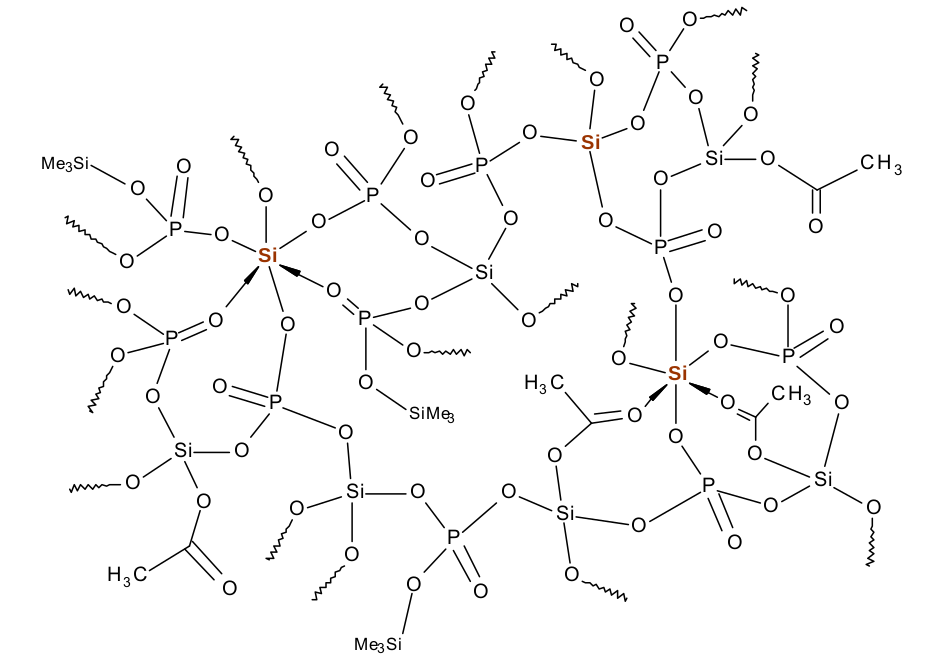
\includegraphics[width=10cm]{si_polymer_cely.png}
  \label{si_polymer_cely}
  \end{figure}


\begin{figure}
\centering
\begin{minipage}{.45\linewidth}
  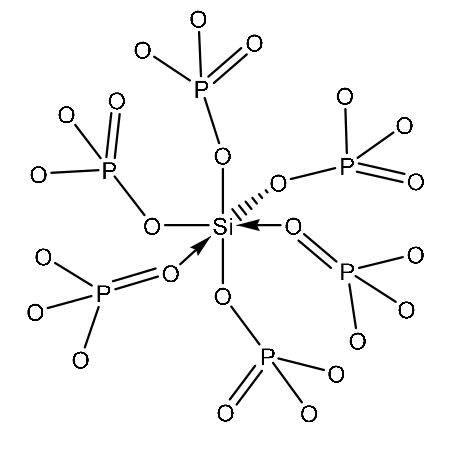
\includegraphics[width=\linewidth]{si_koordinovane_6_P.png}
  \caption{Prostředí kolem Si. \cite{Styskalik2015thesis}}
  \label{img1}
\end{minipage}
\hspace{.05\linewidth}
\begin{minipage}{.45\linewidth}
  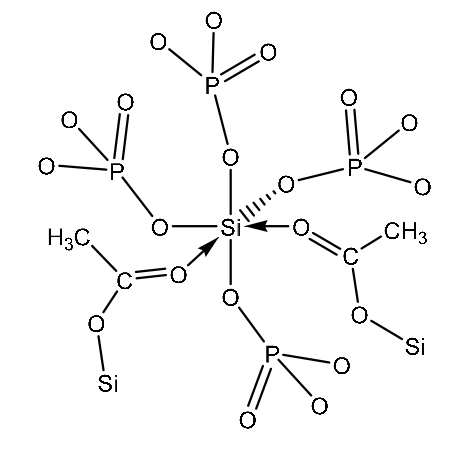
\includegraphics[width=\linewidth]{si_koordinovany_6_C.png}
  \caption{Prostředí kolem Si. \cite{Styskalik2015thesis}}
  \label{img2}
\end{minipage}
\end{figure}

\iffalse
\begin{figure}[h!]
\caption{Prostředí kolem Si. \cite{Styskalik2015thesis} }
  \center
  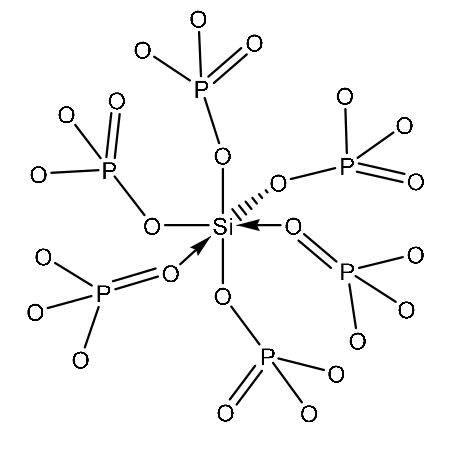
\includegraphics[width=10cm]{si_koordinovane_6_P.png}
  \label{si_koordinovane_6_P}
  \end{figure}
  
  \begin{figure}[h!]
\caption{Prostředí kolem Si. \cite{Styskalik2015thesis} }
  \center
  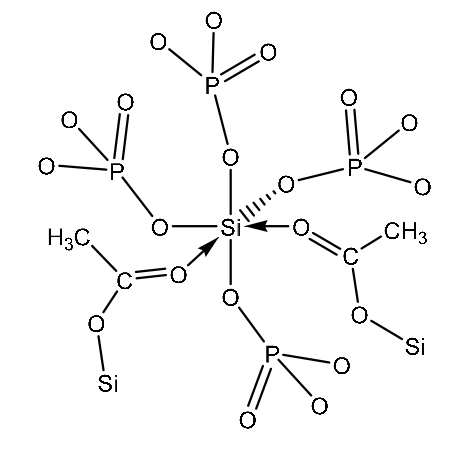
\includegraphics[width=10cm]{si_koordinovany_6_C.png}
  \label{si_koordinovany_6_C}
  \end{figure}
  \fi
\end{otherlanguage}



\chapter{Teoretická část}
Porozumění chemické vazbě mezi atomy daného systému je předpokladem pro vyčerpávající interpretaci získaných experimentálních dat. Na základě znalosti elektronové struktury je také možné předpovědět spektroskopické vlastnosti a~reaktivitu dané molekuly. Pojem chemické vazby je založen na pojmu atom. Počátky tzv. atomové teorie datujeme do období $430-310$ př. n. l. Autorem atomové hypotézy byl řecký filozof Démokritos, který předpokládal, že hmota je stvořena z~malých, dále nedělitelných částí. Tato myšlenka byla v~pozdějším období alchymie potlačena. Renesance atomové teorie se datuje až do 18.století. John Dalton použil atomovou teorii k~popsání průběhu chemických reakcí. Zároveň formuloval zákon stálých poměr slučovacích a~zákon stálých poměrů násobných. Od poloviny 19.století se objevují první myšlenky pojmu valence prvků. Německému chemikovi F. A. Kekulému je přisuzováno prvenství předpokladu o~čtyřvaznosti uhlíku. Samotné porozumění pojmu valence však bylo možné až po objevení elektronu v~roce 1897 J. J. Thomsonem. Toto období může být označeno jako předkvantové období. V~roce 1905 bylo publikováno vysvětlení záření černého tělesa, což odstartovalo kvantový popis atomů a~molekul. Lewis jako první nahlížel na chemickou vazbu jako na párování elektronů. \cite{Munzarova1996thesis} \\
Kvantový popis atomů a~molekul lze obecně rozdělit na lokalizovaný a~delokalizovaný. Myšlenka lokalizovaného popisu elektronů ve vazbě je starší a~odpovídá představě, že mezi dvěma jádry existuje přímá spojnice, pružina. Autorem popisu chemické vazby s~pomocí valenčních vazeb (Valence Bond Theory, VB) je Heitler a~London. VB navazuje na myšlenku sdílení elektronových páru od Lewise. Ústřední myšlenkou jsou vazebné orbitaly, kdy největší elektronová hustota je na spojnici dvou jader sousedních atomů. Spojením dvou atomových orbitalů vzniká vazebný orbital. Tomuto popisu se vymyká například uhlík, proto byl vymyšlen koncept hybridizace. Hlavní myšlenkou je, že dojde k~spojení orbitalů, které jsou si blízké v~energii. Vzniknou tak rovnocenné hybridní orbitaly. \cite{Munzarova1996thesis} \\
Současně s~VB se objevovala teorie molekulových orbitalů (Molecular orbital, MO). Elektronová hustota je delokalizována přes všechny atomy a~představa chemické vazby jako pružinky neexistuje.\cite{Munzarova1996thesis} \\
Opuštění VB jako popisu chemické vazby bylo zpočátku dáno především vyšší výpočetní náročnosti VB, dále se ukázaly také kvantitativní nedostatky při popisu složitějších molekul. \cite{lowe2011quantum} 

\section{Vlnová funkce a~Schrödingerova rovnice}
Chemické vlastnosti molekul určuje jejich geometrická a~elektronová struktura. Ve 20. století již bylo známo, že elektrony se svým chováním vymykají představám klasické mechaniky. Na počátku 20. století bylo popsáno chování černého tělesa, fotoelektrického jevu a~čáry v~atomovém spektru. Myšlenka, že svět je tvořen z~diskrétních částí, kvant, vedla ke vzniku kvantové mechaniky. Zlomovou myšlenkou bylo teoretické popsání záření černého tělesa, které vysvětlit Max Planck \ref{eq_Plack}. Předpokládal, že energie se nepředává spojitě ale po přesně daných částech, kvantech. Na tomto základě Albert Einstein vysvětlil podstatu fotoelektrického jevu, kdy předpokládal, že i světlo je složeno z~částí a~nazval je fotony. Elektromagnetické vlnění začalo mít částicovou povahu.
\begin{equation}
E = h \nu
\label{eq_Plack}
\end{equation}
$E$ je energie, $h$  je Planckova konstanta\footnote{6, 626 070 040  $\cdot 10^{-34} ~ J \cdot s$ \href{http://physics.nist.gov/cgi-bin/cuu/Value?h}{ Physical Measurement Laboratory of NIST}  }, $\nu$ je frekvence. Na tuto představu navázal Louis de Broglie a~navrhl, když vlny mohou mít vlastnosti částic, mohou mít částice vlnové vlastnosti \ref{rce_rovnice_vlny}.
\begin{equation}
\lambda = \frac{h}{mv}
\label{rce_rovnice_vlny}
\end{equation}
$\lambda$ je vlnová délka, $m$ je hmotnosti částice a~$v$ je rychlost částice. Částice a~vlny mají podle rovnic \ref{rce_rovnice_vlny} a~\ref{eq_Plack} duální charakter. Navazující práce se týkala objasnění atomových čárových spekter, kdy atom poskytoval vždy čárová a~dokonale reprodukovatelná spektra. I~zde byly pomocí myšlenky kvantování později objeveny čáry i mimo viditelnou oblast. Na tyto práce později navázal E. Schrödinger, W. Heisenberg nebo P.~A.~M.~Dirac a~kvantová teorie se začala rozvíjet. \cite{celyprincipy}\\
V~běžné mechanice je systém možné přesně popsat polohou a~hybnosti, díky těmto veličinám lze předvídat i pohyb budoucí. V~kvantové mechanice je veškerá interpretace pravděpodobnostní. Vždy lze říci, že se daná částice bude v~nějakém prostoru v~daném čase vyskytovat pouze s~určitou pravděpodobností. Informaci o~částici v~sobě nese Schrödingerova rovnice \ref{SCH_time_dependent}, diferenciální rovnice druhého řádu.\cite{polak2000obecna}
\begin{equation}
i \hbar \frac{\delta}{\delta t} \Psi (\vec{r},t)=\widehat{H} \Psi(\vec{r},t)
\label{SCH_time_dependent}
\end{equation}
$\widehat{H}$ je Hamiltonián, operátor, který reprezentuje kvantově mechanickou cestu k~výpočtu energie systému, $E$ je energie, vlastní hodnota Hamiltoniánu, $\Psi$ je vlnová funkce, která v~sobě ukrývá celou informaci o~systému, $\hbar$ je redukovaná Planckova konstanta. Hamiltonián se skládá ze dvou částí, operátoru kinetické a~potenciální energie.
\begin{equation}
\widehat{H} = \widehat{T} + \widehat{V}
\end{equation}
$\widehat{T}$ reprezentuje kinetickou enregii, $\widehat{V}$ potenciální energii. Kvantově mechanický výraz pro kinetickou energii $\widehat{T}$ je sumou jednočásticových operátorů. 
\begin{equation}
\widehat{T_i} = - \frac{h^2}{8 \pi ^2} \sum \frac{1}{m_i} \left( \frac{\delta^2}{\delta x_i^2} +\frac{\delta^2}{\delta y_i^2} +\frac{\delta^2}{\delta z_i^2} \right)
\end{equation}
$m_i$ je hmotnost částice. Kvantově mechanický výraz pro potenciální energii $\widehat{V}$ je coulombovská interakce mezi částicemi.
\begin{equation}
\widehat{V} = \sum_{i<j}\sum \left( \frac{e_i e_j}{r_{i,j}}\right)
\end{equation}
 Pro účely této práce postačí stacionární Schrödingerova rovnice, která v~sobě nezahrnuje čas \ref{schrodingerova_rovnice}.\\
 \begin{equation}
\widehat{H}\Psi = E \Psi
\label{schrodingerova_rovnice}
\end{equation}
Vlnovou funkci $\Psi$ lze získat řešením Schrödingerovy rovnice \ref{schrodingerova_rovnice}. Fyzikální význam má pouze $|\Psi|^2$, což vyjadřuje hustotu pravděpodobnosti výskytu elektronu. Tento matematický prostor se nazývá orbital. Exaktní řešení \ref{schrodingerova_rovnice} existuje pouze pro atom vodíku a~další exotické atomy, které mají jeden elektron a~jeden proton. Při rozšíření atomu byť i jeden elektron se rovnice \ref{schrodingerova_rovnice} stává analyticky neřešitelnou. Na řadu přichází numerické přístupy a~aproximace. Pro atom s~více elektrony lze k~problému přistoupit tak, že elektrony nebudou vzájemně interagovat. Toto řešení nemá chemický význam, lze tím řešit pouze speciální případy iontů. Hartree přišel na způsob řešení, kdy se elektron pohybuje v časově průměrném poli ostatních jader. \cite{warren1986ab}
Příslušnou vlnovou funkci pro atom s~více elektrony \ref{eq_MO} lze zapsat součin jednoelektronových funkcí \ref{eq_AO}.  V~základu je navrhnuta hrubá vlnová funkce, která poskytuje energii vyšší, než je energie základního stavu. Tato funkce \ref{eq_MO} je variačním přístupem upravována, dokud není nalezena nejnižší energie.  
\begin{equation}
\psi_{AO} = 1s(1)
\label{eq_AO}
\end{equation}
\begin{equation}
\psi_{MO} = 1s(1) \cdot 2s(1)
\label{eq_MO}
\end{equation} 
Zároveň musí platit, že všechny orbitaly musí být vzájemně orthogonální a~normalizované.
\begin{equation}
S_{ii} = \int \psi_i * \psi_i dx dy dz = 1 ~ \wedge ~ S_{ij} = \int \psi_i * \psi_j dx dy dz = 0
\end{equation}
V~tomto přístupu jsou ovšem není dodržena antisymetrii vlnové funkce (Pauliho princip). \cite{warren1986ab}
\begin{equation}
\Psi (1,2) = - \Psi (2,1)
\label{Paulliho_princip}
\end{equation}
 Každá jednoelektronová funkce má prostorovu a~spinovou část, tzv.~spinoorbital. Pro mnohaelektronové atomy už je pro správný výpočet energie vzít spin v~úvahu.  Antisymetrii a~spin do Hartreeho metody zavedl Vladimir Aleksandrovič Fock a~John Slater. Výsledkem byla Hartree-Fockova metoda self-konzistentního pole(HF-SCF), kde se funkce s~nejnižší energii hledá iterativním způsobem za pomoc variačního počtu. Vlnová funkce se zapisuje pomocí Slaterova determinantu, SD, který má obecný tvar \ref{Slateruv_determinant}. SD zaručuje antisymetrii vlnové funkce vůči výměně polohových a~spinových souřadnic. $\psi_i$ je jednoelektronová vlnová funkce, $s_j$ jsou elektrony, $\sqrt{N!}$ je normalizační faktor.
\begin{equation}
\psi =  \frac{1}{\sqrt{N!}}\begin{vmatrix}
\psi_1(1)\alpha(1) & \psi_1(1) \beta (1) & \psi_2(1)\alpha(1) & \dots & \psi_{n/2}(1)\beta(1) \\
\psi_1(2)\alpha(2) & \psi_1(2) \beta (2) & \psi_2(2)\alpha(2) & \dots & \psi_{n/2}(2)\beta(2) \\
\vdots             & \vdots              & \vdots             & \ddots & \vdots \\
\psi_1(n)\alpha(n) & \psi_1(n) \beta (n) & \psi_2(n)\alpha(n) & \dots & \psi_{n/2}(n)\beta(n) 
\end{vmatrix}
\label{Slateruv_determinant}
\end{equation}
U~atomů s~více  elektrony chemie začíná, hlavním cílem je získat znalosti o~molekulách. V~tomto systému se nově objevuje více než jedno jádro a~systém se stává opět příliš složitý pro matematické řešení. Ve skutečnosti je proton přibližně $1800 \times$ těžší než elektron, tudíž je rychlost mnohem menší, než rychlost elektronu. Situace lze zjednodušit oddělením pohybu elektronů od pohybu jader a~řešit tak problémy odděleně. Přístup byl navržen jako Born-Oppenheimerova aproximace \ref{eq_B_O_aproximace}. Vlnová funkce elektronů závisí pouze na poloze jader, ne jejich rychlosti.\cite{lechamolecularmodeling} Zároveň je vlnová funkce parametricky závislá na poloze jader, pro každou geometrii jader je získána jiná vlnová funkce. Závislost energie na poloze jader se pro víceatomové molekuly nazývá hyperplocha potenciální energie.\cite{dftshrnutivysledky}
\begin{equation}
\Psi_{tot}(nuclei, elektrons) = \Psi(electrons) \cdot \Psi(nuclei)
\label{eq_B_O_aproximace} 
\end{equation}

\section{Metody kvantové chemie}
Metody výpočetní chemie lze ve stručnosti shrnutou na \textit{Ab inito} metody, semi-empirické metody a~DFT metody. \textit{Ab inito} metody řeší Schrödingerovu rovnici bez použití parametrů z~experimentálních dat.  Vzájemnou souvislost a~podobnost metody vystihuje schéma na obrázku \ref{schema_QM}.
 \begin{figure}[h]
\caption{Schéma post-Hartree-Fockových teorií, $n^m$ je škálování vzhledem k~velikosti systémy \cite{pdf_obrazek}. }
  \center
  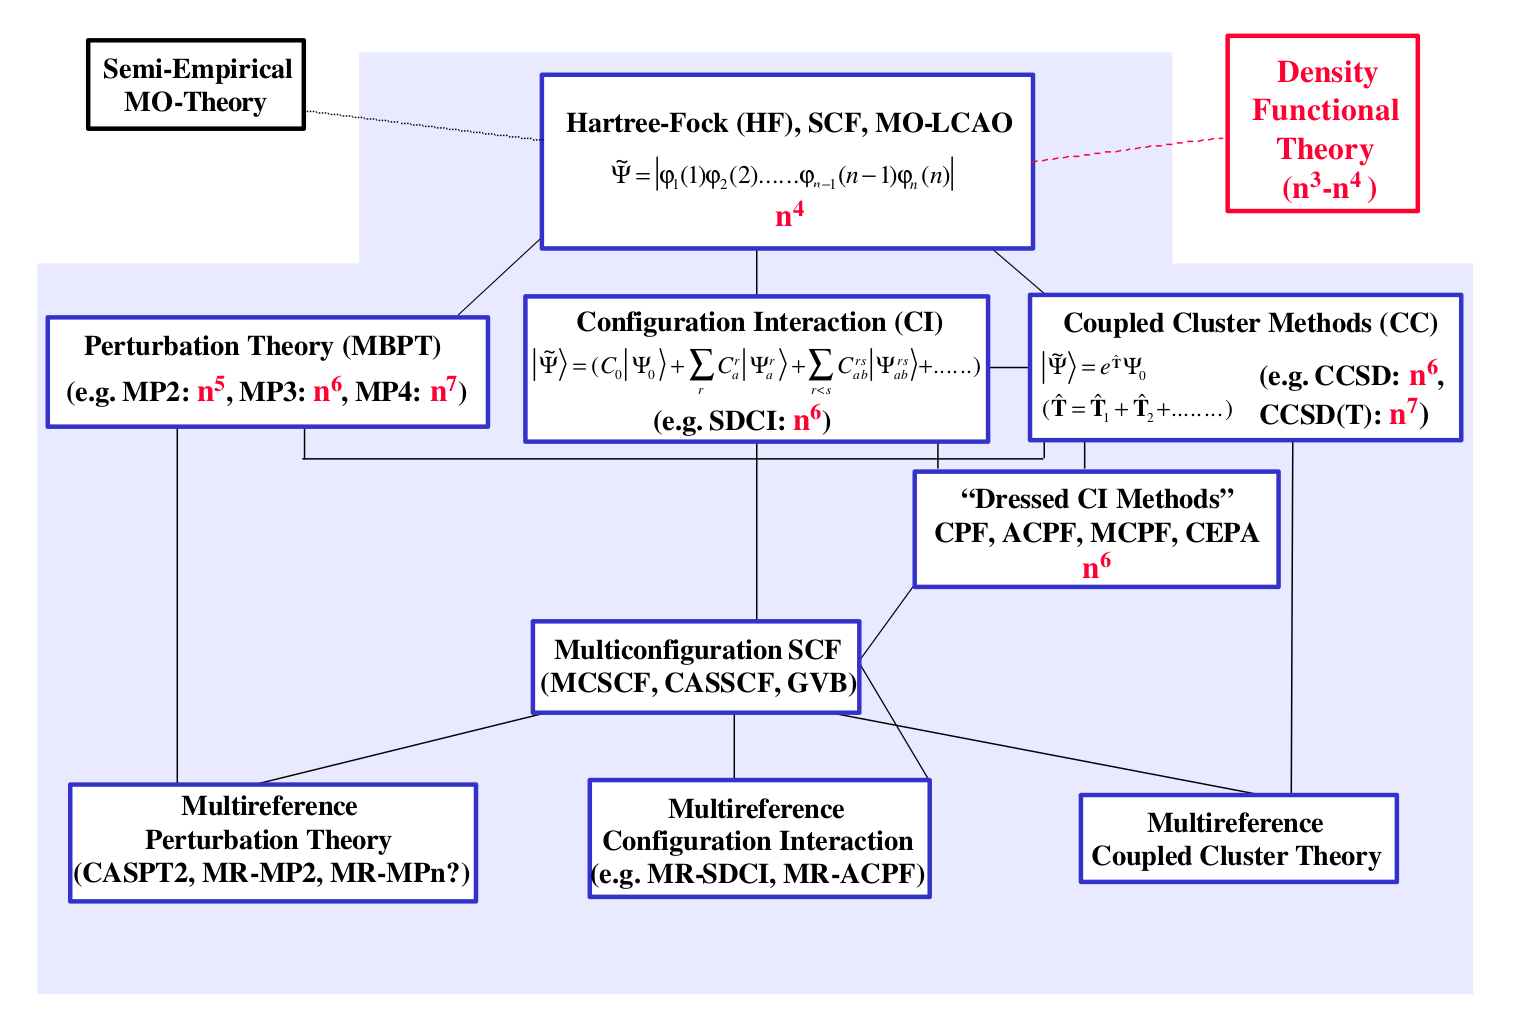
\includegraphics[width=12cm]{schema_QM.png}
  \label{schema_QM}
  \end{figure}
  Metody QM vychází z~řešení stacionární Schrödingerovy rovnice \ref{schrodingerova_rovnice}. Semiempirické metody řeší Schrödingerovu rovnici pouze částečně, některé parametry jsou dodány z~experimentů. \\
     Základní aproximací je Born-Oppenheimerova aproximace a~zapsání vlnové funkce jako Slaterův determinant pomocí atomových orbitalů. Z~tohoto základu vznikla Hartree, která navíc uvažuje elektron v~průměrném poli zbylých elektronů. Zde pomocí variačního přístupu hledá nejvhodnější energii. Antysymetrii vlnové funkce zajistí SD a~Fockovy rovnice, proto Hartee-Fockova metoda. Samotný HF přístup v~sobě neobsahuje korelaci pohybu elektronů. Tento faktor je tam možno vložit dodatečně pomocí tradičních \textit{ab inito} metod jako například Many-Body Pertrubation  theory (MBPT), konfigurační interakcce (Configuration Interaction, CI) nebo spřažené klastry(Coupled Cluster methods, CC). Śkálování těchto metod je uvedeno na obrázku \ref{schema_QM}. Tyto metody jsou přesné, ale výpočetně velice náročné, proto nejsou vhodné pro příliš velké systémy. Řešením je použití teorie funkcionálu hustoty (The Density Functional theory, DFT) nebo Rozšířenou Hückelovu metodu (The Extended Hückle theory, EHT).

\section{Rozšířená Hückelova metoda}
EHT se řadí mezi semiemprické metody, které  pro výpočet energie používají klasický \textit{ab inito} přístup a~některé parametry jsou vzaty z~experimentu. Tím se snižuje výpočetní náročnost. Přes její jednoduchost dává dobré kvalitativní výsledky především v~oblasti molekulových orbitalů. EHT navazuje na Hückelův přístup, který platil pouze pro konjugované systémy. EHT může být použita i pro systémy se $\sigma$~vazbami. Na rozvoji teorie se podílel Roald Hoffman.\cite{lowe2011quantum} \\
Základem metody jsou sekulární rovnice. EHT poskytuje jednoduché řešení členu $H_{ij}$ pomocí vzorce \ref{EHT_vypocet_H} a~empirických parametrů. $S_{ij}$ je překryvový integrál, $E$ je hledaná energie.
\begin{equation}
E = \begin{vmatrix}
H_{11} - E S_{11} & H_{12} - E S_{12} & \dots & H_{1j} - E S_{1j} \\
H_{21} - E S_{21} & H_{12} - E S_{22} & \dots & H_{1j} - E S_{2j} \\
\vdots & \vdots &  \ddots & \vdots  \\
H_{i1} - E S_{i1} & H_{i2} - E S_{i2} & \dots & H_{ij} - E S_{ij} \\
\end{vmatrix}
\end{equation}


\begin{equation}
H_{ij} = K~S_{ij} \left( \frac{H_{ii} + H_{jj}}{2} \right)
\label{EHT_vypocet_H}
\end{equation}
kde $K$ je parametr, jehož hodnota byla R. Hoffmannem stanovena na 1,75.\cite{lowe2011quantum}

\section{Metoda funkcionálu hustoty}
DFT metody jsou založeny na vztahu mezi elektronovou hustotou a~celkovou energii systému, teorie funkcionální \footnote{Funkcionál je operátor, který zobrazuje z~prostoru funkcí do množiny obecně komplexních čísel.} hustoty. Elektronová hustota $\varrho(\vec{r})$ je pravděpodobnosti, že v~nějakém bodě prostoru nalezneme nějaký elektron.  Výhodou tohoto přístupu je, že elektronová hustota je funkcí pouze tří prostorových souřadnic. Tento výpočetní model byl objeven už v~roce 1920, pro chemii začal mít význam až v~60. letech 20. století. DFT přístup je výpočetně podobně náročný jako HF, ale přesnější, obsahuje korelační energii. \\

V~roce 1964 uveřejnili Koch a~Hohenberg dva teorémy, které ukázaly, že energie základního stavu  a~další vlastnosti jsou jednoznačně určeny elektronovou hustotou. Energie je funkcionál elektronové hustoty.\cite{lechamolecularmodeling}
\subsection{Principy}
\subsubsection{První Hohenberg- Kohn teorém}
Pro libovolný systém interagujících elektronů je externí potenciál $V_{ext}$ jednoznačně
určen elektronovou hustotou (až na konstantu). \cite{dftshrnutivysledky}
\begin{equation}
E_{el} = E_{el} (\varrho)
\end{equation}
 Za znalosti elektronové hustoty lze vypočítat energii a~všechny ostatní vlastnosti základního stavu.
\subsubsection{Druhý Hohenberg-Kohn teorém}
Druhý teorém je postaven na variačním principu. Poskytuje informace, jak lze najít elektronovou hustotu, která poskytne nejnižší a~zároveň nejpřesnější energii.
\cite{koch2000chemist} 
Energie přesné elektronové hustoty základního stavu $\varrho_O$ je vždy menší, než energie nalezená jinou fyzikálně přijatelnou elektronovou hustotou $\varrho'$.\cite{Semradthesis}
\begin{equation}
E [\varrho_0] < E[\varrho ']
\end{equation}

\subsubsection{Kohn-Shamovy rovnice}
Při hledání vhodného funkcionálu je zásadní problém zahrnout kinetickou energii elektronů, klasickou coulombickou interakci mezi elektrony a~dále korelační a~výměnné efekty. Hlavní myšlenkou bylo rozdělení hledaného funkcionálu $E(\varrho(\vec{r}))$ do menší částí. \cite{koch2000chemist}
\begin{equation}
E(\varrho(\vec{r})) = T_s[\varrho(\vec{r})] + J[\varrho(\vec{r})] + \int V_{EX}(\vec{r})\varrho(\vec{r})d\vec{r} + E_{EX}[\varrho(\vec{r})]
\end{equation}
 Kinetickou energii $T_s$ lze započítat jako Shamův potenciál. Lze sestavit pole neinteragujících elektronů, které bude mít stejnou elektronovou hustotu jako reálný systém interagujících elektronů. $T_{s}$ lze počítat jako součet jednoelektronových funkcí \ref{kineticka_energie_jednoelektronova}. \cite{koch2000chemist}
\begin{equation}
T_s = -\frac{1}{2} \sum_{i=1} ^{N}  \bra{\psi_i}{\nabla^{2}}\ket{\psi_i}
\label{kineticka_energie_jednoelektronova}
\end{equation}
Tímto způsobem vypočítaná $E_{kin}$ není skutečná $E_{kin}$ systému. \\
$J[\varrho(\vec{r})]$ je přesná Coulombovská repulze. $E_{EX}[\varrho(\vec{r})]$ je výměnně-korelační energie, $\int V_{EX}(\vec{r})\varrho(\vec{r})d\vec{r}$ je přesná energie atrakce elektronů jádry.
\subsection{DFT v~praxi}
Výběr vhodného funkcionálu je nelehký úkol. Funkcionály mohou být obecně rozděleny na tři kategorie. Aproximace lokální hustoty (Local Density Approximation, LDA), metoda zoběcněného gradientu (Generalized Gradient Approximation, GGA) a~poté hybridní funkcionály. \cite{dftshrnutivysledky}
\subsubsection{Aproximacce lokální hustoty}
LDA funkcionály vychází z~modelu homogenního elektronového plynu, kdy máme v~celém systému konstantní elektronovou hustotu.\cite{dftshrnutivysledky} V~základu se jedná o~\textit{ab inito} přístup, přesto má pro chemii využití pouze pro valenční elektrony. Často totiž v~molekulách není pravidelná distribuce elektronové hustoty. Prostor lze rozdělit na jednotky objemu a~elektronovou hustotu sčítat přes objem podle rovnice.
\begin{equation}
E_{XC}^{LDA} = \int \varrho (\vec{r} \epsilon_{XC} (\varrho (\vec{R})) d \vec{r}
\label{LDA_vyraz_pro_obecnou_energii}
\end{equation}
Tvar $\epsilon_{XC}(\varrho (\vec{r}))$je výměnně-korelační energie pro jeden elektron, která může být rozdělena na výměnnou a~korelační část. 
\begin{equation}
\epsilon_{XC}(\varrho (\vec{r})) = \epsilon_x (\varrho) + \epsilon_c (\varrho)
\label{LDA_tvar_vymene_korelacni_energie}
\end{equation}
Výměnný člen lze zapsat analyticky, známy pod názvem Slaterův výměnný člen, značen S.
\begin{equation}
\epsilon_{XC}(\varrho (\vec{r})) = - \frac{3}{4} \sqrt[3]{\frac{3 \varrho (\vec{r})}{\pi}}
\label{LDA_vymenny_clen}
\end{equation}
Korelační energii lze zavést metodou VWN (auto rVosko, Wilky a~Nuisar) pomocí numerických výpočtů. Vylepšením je spinově závislá aproximace lokální hustoty, která zavádí elektrony se spinem $\alpha$ a~$\beta$.
\begin{equation}
E_{XC}^{LSD}[\varrho_{\alpha}, \varrho_{\beta}] = \int \varrho (\vec{r} \epsilon_{XC}( \varrho_{\alpha}(\vec{r}), \varrho_{\beta}(\vec{r})) d \vec{r}
\end{equation}
\cite{koch2000chemist}
\subsubsection{Metoda zobecněného gradientu}
GGA funkcionál vychází z~aproximace lokální hustoty, která je dále vylepšována. Jedna z~možností je použít \textbf{gradient elektronové hustoty} $\nabla \varrho (\vec{r})$.  \cite{koch2000chemist}

\subsubsection{Hybridní funkcionály}
Přístup kombinuje HF vzorec pro výpočet energie ( \textbf{dát odkaz}) a~výměnné funkcionály. 
Do této kategorie patří nejznámější funkcionál \textbf{B3LYP}.
\begin{equation}
E_{ex}^{B3LYP} = (1-a_0-a_x)E_x^{LDA} + a_0E_x^{exact} + a_x^{B88} + (1-a_c)E_c^{VWN} + a_c^{LYP}
\label{B3LYP_rovnice}
\end{equation}
$a_0$, $a_x$ a~$a_c$ jsou nastavitelné parametry. \textbf{B3LYP} má 20\% podíl výměnné energie. \cite{dftshrnutivysledky}

\section{Báze v~\textit{ab inito} výpočtech }\label{kapitola_baze}
Množina funkcí, ze kterých jsou skládány orbitaly, se nazývá bazí atomových orbitalů. Pro výběr funkcí platí dvě základní pravidla. Příslušné bázové funkce musí dostatečně dobře popsat vlnovou funkci, aby získané výsledky měly chemický význam. Zároveň integrály $F_{ij}$ a~$S_{ij}$ musí být řešitelné v~rozumně dlouhém časem. \cite{lowe2011quantum}
Pro popis atomu lze použít minimální nebo rozšířené báze. Minimální báze obsahuje pouze funkce, které popisují orbitaly obsazené v~základním stavu daného atomu. Rozšířená báze obsahuje například polarizační funkce nebo difuzní funkce. Mezi základní typy bazí pro atomové orbitaly jsou orbitaly vodíkové typu, orbitaly Slaterova typu (STOs) a~gaussovské funkce. \cite{dftshrnutivysledky}
Orbitaly vodíkového typu mají radiální a~angulární část. Orbitaly vodíkového mají nevýhodu ve své složitosti a~často je nutné použít numerické řešení problému. STO orbitaly nemají radiální uzly a~pro některé integrály neexistuje analytické řešení. STO orbitaly jsou ve tvaru polynomu souřadnic a~exponenciály \ref{STO_orbital}.\cite{jensen2007introduction}
\begin{equation}
\chi_{\zeta, n, l, m}(r, \theta, \varphi) = NY_{l,m} (\theta, \varphi) r^{n-1} e^{-\zeta r}
\label{STO_orbital} 
\end{equation}
$N$ je normalizační faktor, $Y_{l,m}$ sféricky harmonická funkce, exponent závisí na vzdálenosti od jádra jako $r$. Radiální část je tvořena jako lineární kombinace STO. Především přidáváním bázových funkcí STO typu enormně narůstá výpočetní čas. Alternativou jsou Gaussovské orbitaly (Gausian type orbitals, GTO).
\begin{equation}
\chi(r) = Nr^n e^{-a(r-r_A)^2}
\end{equation}
 Výhodou GTO je to, že jejich součin je stále GTO. Na rozdíl od ostatních funkcí nemají správné chování na jádře. Z~tohoto důvodu je báze STO orbitalů tvořena několika GTO, které jsou označovány jako primitivní Gaussovské funkce. Největším přínosem GTO je rozdíl v~druhé mocnině vzdálenosti v~exponenciálním členu.\cite{lowe2011quantum}. 
 V~současné době existuje obrovské množství bazí, které lépe či hůře popisuje zvolený problém. Mezi základní báze jsou uváděny DZP, STO-3G a~různé druhy 6-31G. DZP je double-zeta gassovská báze s~polarizací, STO-3G jsou Slaterovy orbitaly zjednodušeny jako lineární kombinace tří primitivních gaussiánů, odpovídá minimální bázi. 3-21G jsou označovány jako \uv{split valence basics sets}. Vnitřní elektrony jsou popisovány tří primitivními gaussiány, valenční orbitaly  do dvou primitivních gaussiánů a~jednoho jednoduchého gaussiánu. Pro bázi 6-31G je vnitřní oblast tvořena šesti primitivními gaussiány, ostatní je obdobné jako pro 3-21G. Báze 6-21*G je v~základu obdobná, * označuje polarizační funkci. Přidává p orbital pro vodíky a~d orbitaly pro těžší atomy. Symbol ** označuje přidání d orbitalů pro vodík.\cite{lowe2011quantum} \\
 
 DFT metodami lze krom optimalizací počítat také parametry nukleární magnetické rezonance (NMR). Jedním z~NMR charakteristik molekul je chemické stínění. Do \textit{ab-inito} výpočtu nově vstupuje vnější magnetické pole $B_0$, které je reprezentováno vektorovým potenciálem tohoto pole. V~ideálním případě by neměla mít volba počátku tohoto pole vliv na výsledek. Jedním z~důsledků aproximace v~kvantové chemii je fakt, že volba počátku výrazně ovlivňuje výsledné chemické stínění. Problém se nazývá \uv{Gauge origin problem}. Metoda GIAO (Gauge  Including Atomic Orbitals)řeší problém způsobem, že zahrnuje počátek vektorového potenciálu do atomových orbitalů. Vhodnou bazí pro tyto výpočty je IGLO$-$III (Individual Gauge for Localized Orbitals).\cite{Standara2006thesis} \cite{g09}

\subsection{Kvalitativní koncepty v~kvantové chemii}
Důležitou součástí výzkumu v~oblasti kvantové chemie jsou zjednodušené koncepty, které pomáhají s~interpretací kvantově$-$chemických dat. Jedním z~příkladů je vysvětlení vaznosti atomů a~molekul. \\
Lewisovská teorie chemické vazby nahlíží na vazbu jako na lokalizovaný koncept, kde jsou elektrony na spojnici jader. Tento jednoduchý koncept předpokládá, že platí tzv. oktetové pravidlo a~maximální počet vazeb odpovídá číslu skupiny, ve které se atom nachází. Tato teorie si bohužel nedokáže poradit už s~molekulou methanu. Podle Lewisovské teorie by měl uhlík tvořit dvojvazné molekuly. V~případě čtyřvazných molekul by měly být dvě vazby rovnocenné a~dvě o~nižší energii kvůlu zapojení rozdílných orbitalů. V~methanu ale najdeme čtyři stejně dlouhé a~naprosto rovnocenné vazby. Vysvětlení této skutečnosti nabízí teorie hybridizace. Ta předpokládá, že může dojít ke sjednocení orbitalů o~blízké energii, za vzniku hybridního orbitalu. Tímto způsob vytvořené vazby si jsou naprosto rovnocenné. Ani koncept hybridizace nevysvětluje všechny případy vaznosti molekul. Pro některé atomy jsou si orbitaly natolik vzdálené, že hybridizace nepřichází v~úvahu. Nejlepším popisem pro tyto systémy jsou molekulové orbitaly. Ty zavádí do celého popisu princip delokalizace. Mezi molekuly, které se vymykají Lewisovskému přístpupu, lze zařadit obecně sloučeniny vzácných plynů (fluoridy xenonu),  \ce{SF6}, \ce{ClF3} a~\ce{I3^-}. \\

Ochotu tvořit hypervalentní molekuly lze odhadnout podle konceptu HSAB (Hard and Sfot Acids and Basics). Kyseliny a~báze mohou být rozděleny na měkké a~tvrdé. HSAB teorie říká, že tvrdá kyselina a~tvrdá báze spolu poskytnou stabilní komplex, naopak slabá kyselina a~slabá báze spolu poskytnou méně stabilní komplex. Z~toho vyplývá, že ze znalosti reakčních podmínek a~příslušné tvrdosti lze predikovat stabilitu vzniklého komplexu. Jeden z~možností kvantitativního určení tvrdosti/měkkosti je určení parametrů $\chi$ \footnote{Elektronegativity byla Paulingem definována pomocí ionizačního potenciálu a~elektronové afinity} \ref{hsab_vypocet_elektronegativita} a~$\eta$ \ref{hsab_vypocet_tvrdost}. \cite{hsabclanek}. 
\begin{equation}
\chi = - \left( \frac{\delta E}{\delta N} \right) = \frac{IP + EA}{2} = -\mu
\label{hsab_vypocet_elektronegativita}
\end{equation} 
\begin{equation}
\eta = \frac{1}{2} \left( \frac{\delta \mu}{\delta N} \right) = \frac{1}{2}\left( \frac{\delta^2 E}{\delta N^2} \right) = \frac{I~- A}{2}
\label{hsab_vypocet_tvrdost}
\end{equation} 
$\chi$ je absolutní elektronegativita, $E$ je energie a~$N$ je počet elektronů. \cite{hsabwatoc} Podle Koopmansova teorému $E_{HOMO} = - IP$, $IP$ je ionizační potenciál a~$E_{LUMO} = -EA$, $EA$ je elektronová afinita.\cite{kratochvilexcerpta} $\eta$ je atomová tvrdost \footnote{$\eta = \frac{1}{\sigma}$, $\sigma$ je měkkost atomu}.\cite{pearson1986absolute} Tvrdá kyselina a~báze je charakterizována velkým rozdílem $IP$ a~$IA$, což se projeví jako vysoké hodnoty $\chi$ a~$\eta$. Při znalosti $E_{HOMO}$ a~$E_{LUMO}$ lze predikovat ochotu reakčního centra interagovat s~námi zvoleným reagentem a~zároveň odhadnout stabilitu vzniklého komplexu. Systémy s~velkým rozdílem $E_{HOMO}$ a~$E_{LUMO}$ jsou tvrdší, stabilnější a~méně reaktivní.\cite{hsabwatoc}




\chapter{Výsledky a~diskuze}
Cílem výpočetní části bylo zkoumat struktury křemičitofosfátů metodou EHT a~DFT. Pro metodu EHT byly vybrány menší struktury, metodou DFT byly zkoumány větší struktury. Ze získaných hodnot energie HOMO a~LUMO orbitalů byla určena tvrdost/měkkost a odhadnuta reaktivita.
\section{Výpočty metodou EHT a~jejich grafický výstup ve formě obrázku C.A.C.A.O. s~použitím předvolených parametrů pro všechny atomy} \label{kapitola_EHT}
Pro účel vazebné analýzy byly všechny čtyři molekuly studovány prostřednictvím tzv. fragmentové analýzy. V~jejich rámci byly provedeny kvantově chemické výpočty nejen pro kompletní molekuly, ale i pro podjednotky P=O a~trojici bazálních ligandů. Výsledné MO pak byly vyjádřeny pomocí těchto fragmentových orbitalů (FMO). FMO byly vybírány z~interakčních diagramů podle příspěvků do překryvové populace. Z~těchto hodnot lze určit míru interakce. Všechny struktury molekul byly před výpočtem optimalizovány programem Gaussian \cite{g09} \footnote{B3LYP 6-31G*}.
%H4SIO4
% --------------------------------------------------------------------------
\subsection{Molekula H$_4$SiO$_4$}
Základní molekula pro reprezentaci čtyřkoordinovaného křemíku byla \ce{H4SiO4}. Z~interakčního diagramu \ref{h4sio4_diagram_upraveny} byly vybrány FMO $\bra{20}{\hat{H}}\ket{24}$, $\bra{16}{\hat{H}}\ket{24}$, $\bra{11}{\hat{H}}\ket{21}$, $\bra{19}{\hat{H}}\ket{21}$, $\bra{15}{\hat{H}}\ket{22}$ a~$\bra{18}{\hat{H}}\ket{22}$, pro které byla udělána analýza složení molekulových orbitalů. Molekula má symetrii S$_4$. Fragmentové orbitaly 7, 22 a~26 se navzájem mísí za vzniku MO číslo 1, 20 a~24, znázorněných na obrázku \ref{obr_h4sio4_vysledky_I}. Fragmentové orbitaly  11, 19 a~21 se navzájem mísí za vzniku MO číslo 4, 16 a~21, znázorněných na obrázku \ref{obr_h4sio4_vysledky_II}. Fragmentové orbitaly  15, 18 a~22 se navzájem mísí za vzniku MO číslo 2, 19 a~22, znázorněných na obrázku \ref{obr_h4sio4_vysledky_III}.    

\begin{figure}
\begin{center}
\subfigure[Interakční diagram pro \ce{H4SiO4}.]{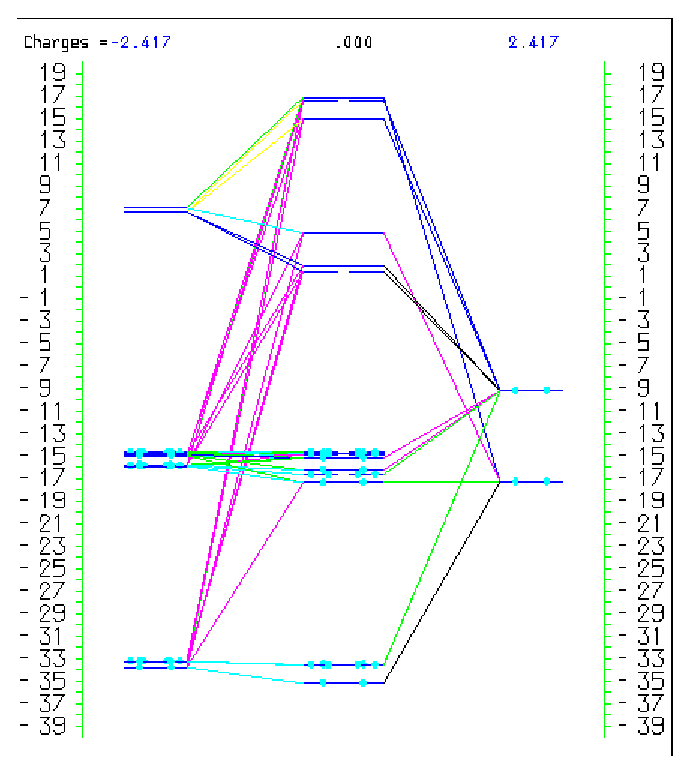
\includegraphics[width=5cm]{h4sio4_diagram_upraveeny.eps} \label{h4sio4_diagram_upraveny}}
\subfigure[Optimalizovaná struktura \ce{H4SiO4}.]{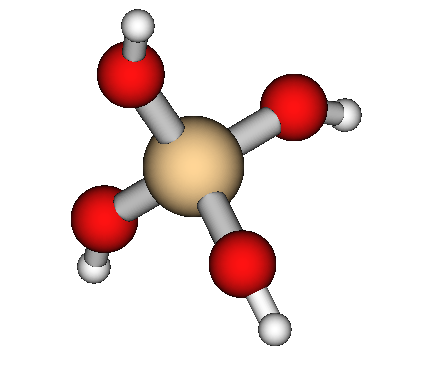
\includegraphics[width=5cm]{h4sio4_obr.png}\label{h4sio4_obr}}
\label{obr_h4sio4_vysledky_I}
\end{center}
\end{figure}
 
 
 
\begin{table}[htbp]
\begin{minipage}{\textwidth}
\caption{Výsledné mísení orbitalů pro \ce{H4SiO4}}
\begin{center}
\begin{tabular}{|r|r|r|r|r|r|}
\hline 
\multicolumn{2}{|c|}{$\bra{20}{\hat{H}}\ket{24}$, $\bra{16}{\hat{H}}\ket{24}$} & \multicolumn{2}{|c|}{$\bra{11}{\hat{H}}\ket{21}$, $\bra{19}{\hat{H}}\ket{21}$}& \multicolumn{2}{|c|}{$\bra{15}{\hat{H}}\ket{22}$, $\bra{18}{\hat{H}}\ket{22}$} \\
\hline \hline
\multicolumn{1}{|l|}{MO\footnote{Molekulový orbital} } & \multicolumn{1}{r|}{W\footnote{součet procentuálních příspěvků příslušných fragmentových orbitalů do příslušného molekulového orbitalu}} & \multicolumn{1}{l|}{MO} & \multicolumn{1}{r|}{W} & MO & \multicolumn{1}{r|}{W} \\ \hline
1 & 84 \% & 4 & 67 \% & 2 & 65 \% \\ \hline
20 & 91 \% & 16 & 79 \% & 19 &  97 \% \\ \hline
24 & 99 \% & 21 & 100 \% &  22& 100 \% \\ \hline
\end{tabular}
\end{center}
\label{tab_h4sio4_vysledky}
\end{minipage}
\end{table}
  %  Pro fragmentové orbitaly $\bra{22}{\hat{H}}\ket{26}$, $\bra{7}{\hat{H}}\ket{26}$ byly nalezeny příslušné molekulové orbitaly \ref{obr_h4sio4_MO_s1_1}, \ref{obr_h4sio4_MO_s1_20} a \ref{obr_h4sio4_MO_s1_24} .
    
 %-------------
\begin{figure}
\begin{center}
\subfigure[MO 1]{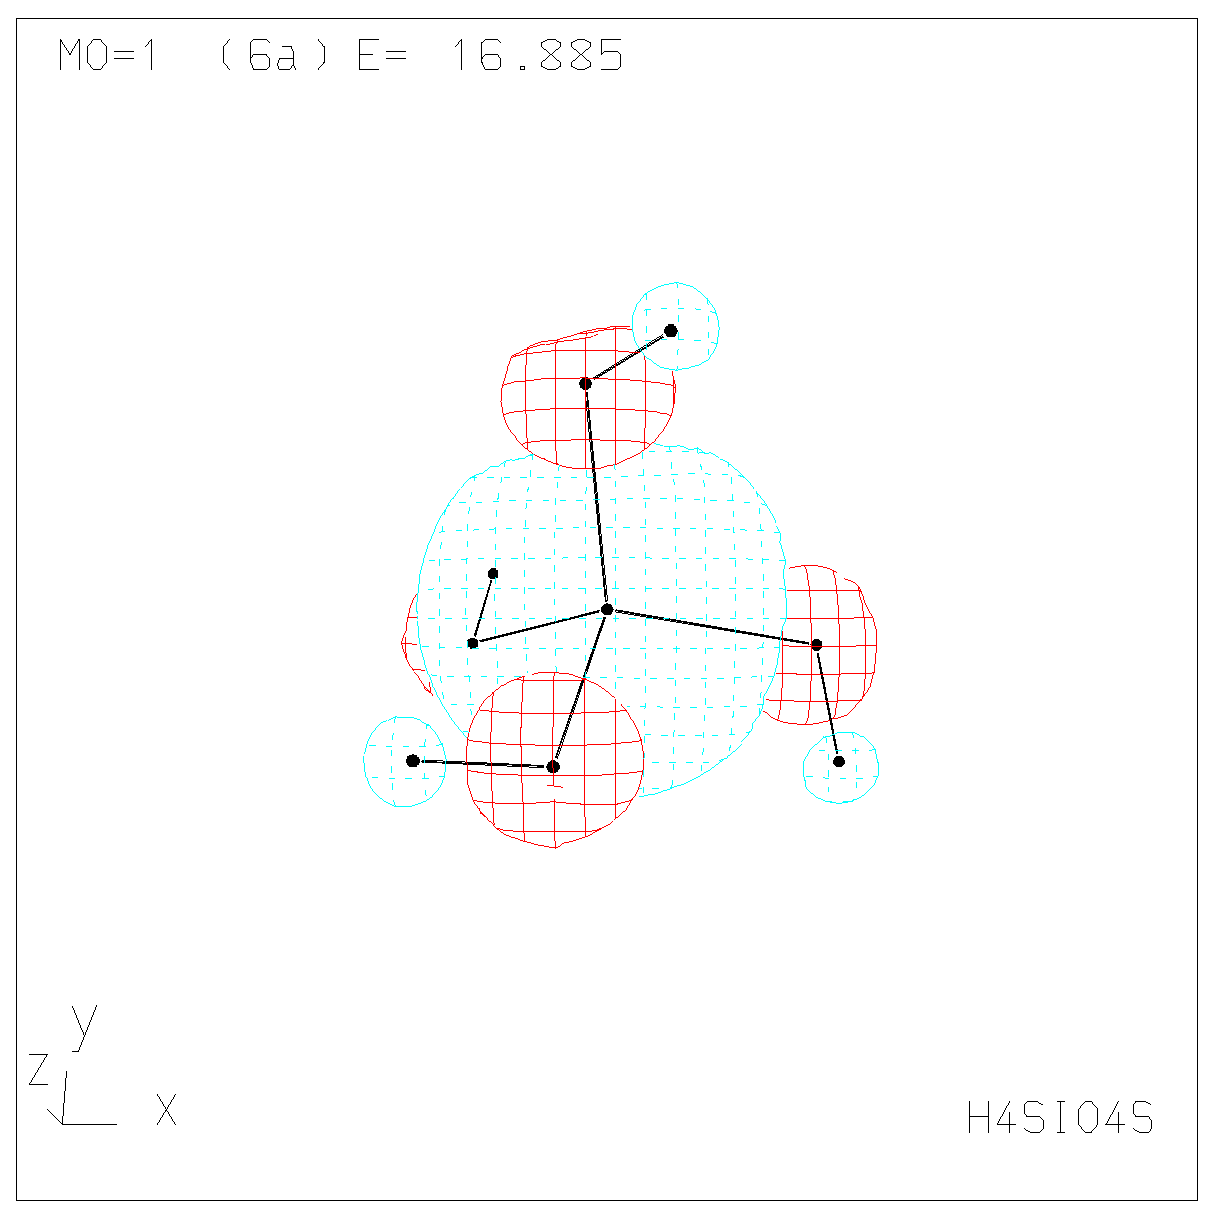
\includegraphics[width=5cm]{h4sio4_obrazky/s1_1.eps} \label{obr_h4sio4_MO_s1_1}}
\subfigure[MO 20]{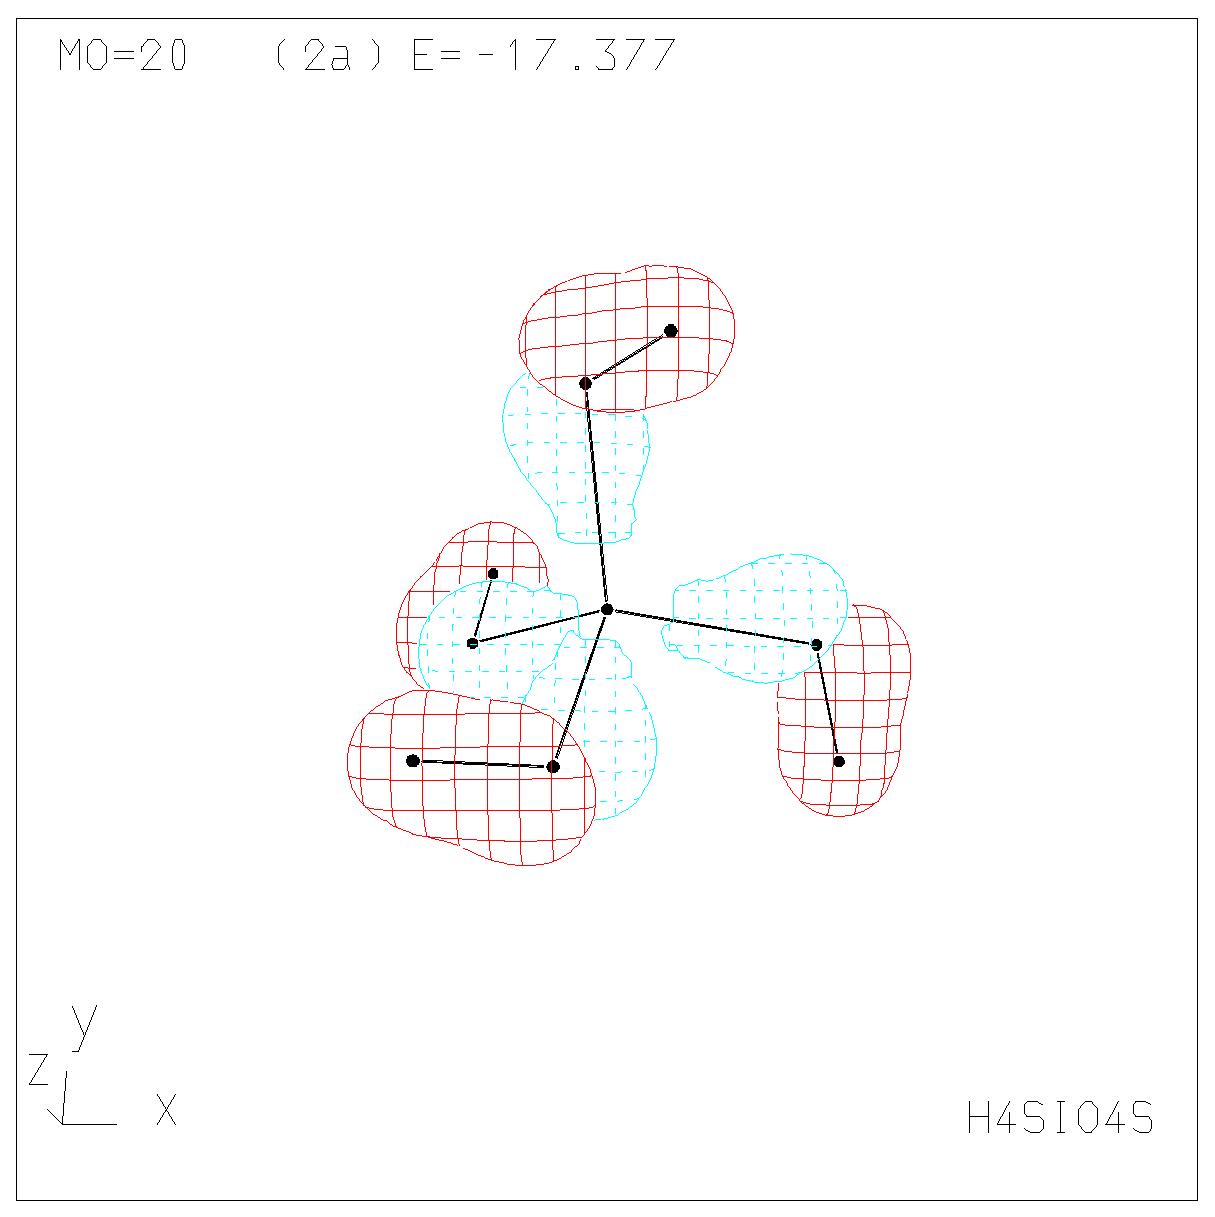
\includegraphics[width=5cm]{h4sio4_obrazky/s1_20.eps}\label{obr_h4sio4_MO_s1_20}}
\subfigure[MO 24]{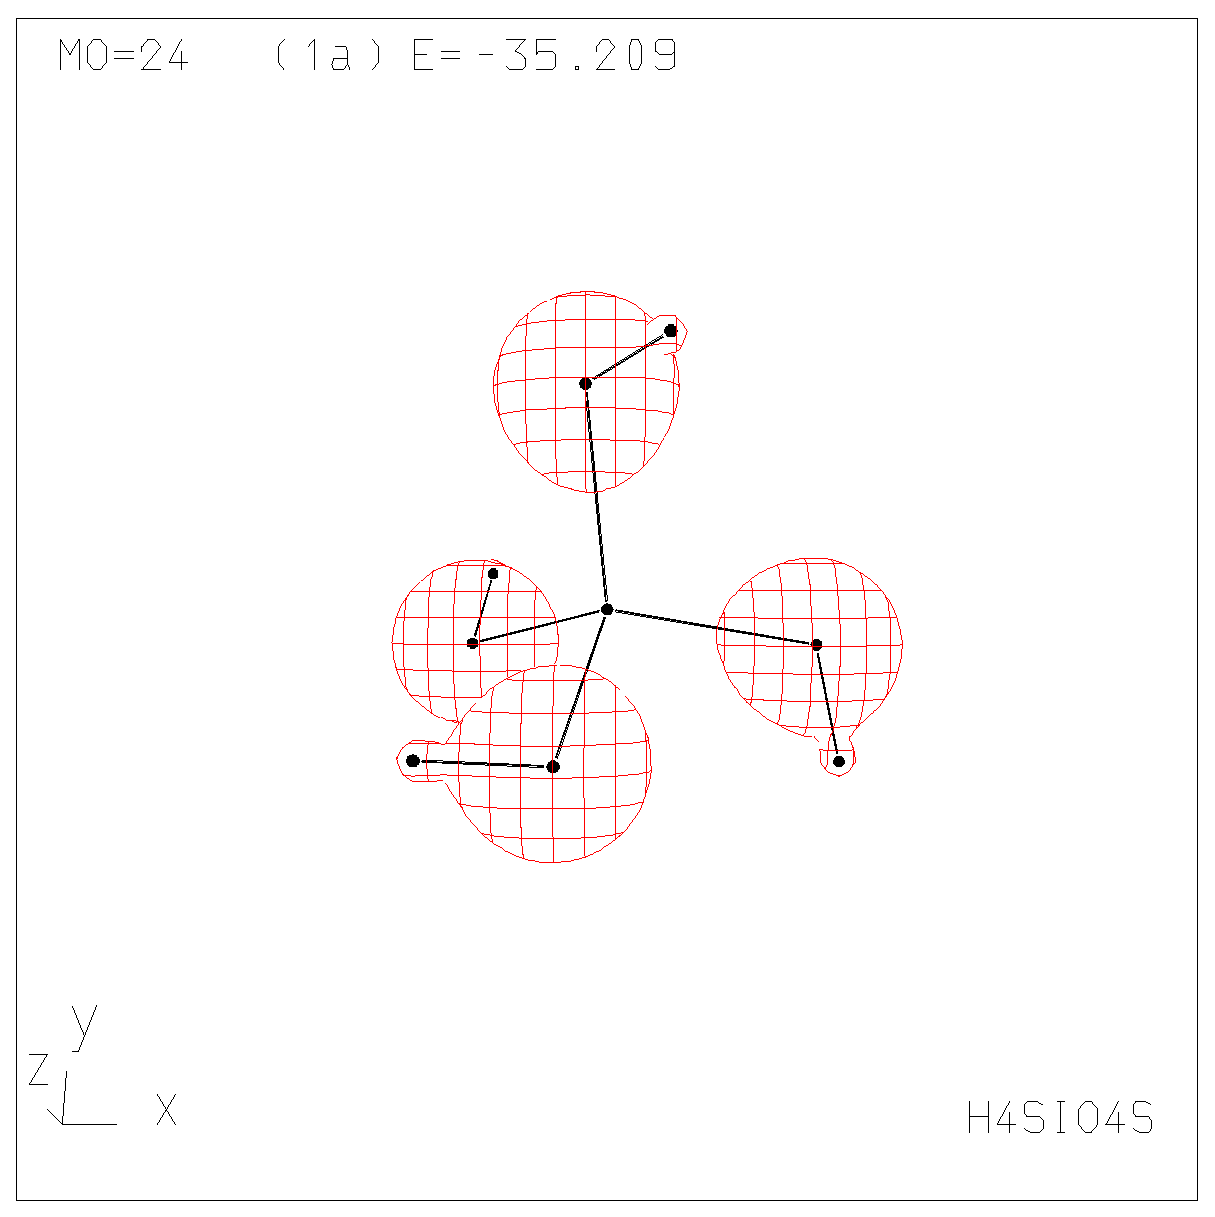
\includegraphics[width=5cm]{h4sio4_obrazky/s1_24.eps}\label{obr_h4sio4_MO_s1_24}}
\caption{Interakce $\bra{22}{\hat{H}}\ket{26}$, $\bra{7}{\hat{H}}\ket{26}$ z~tabulky \ref{tab_h4sio4_vysledky}.}

\label{obr_h4sio4_vysledky_I}
\end{center}
\end{figure}


%------------    

\begin{figure}
\begin{center}
\subfigure[MO 4]{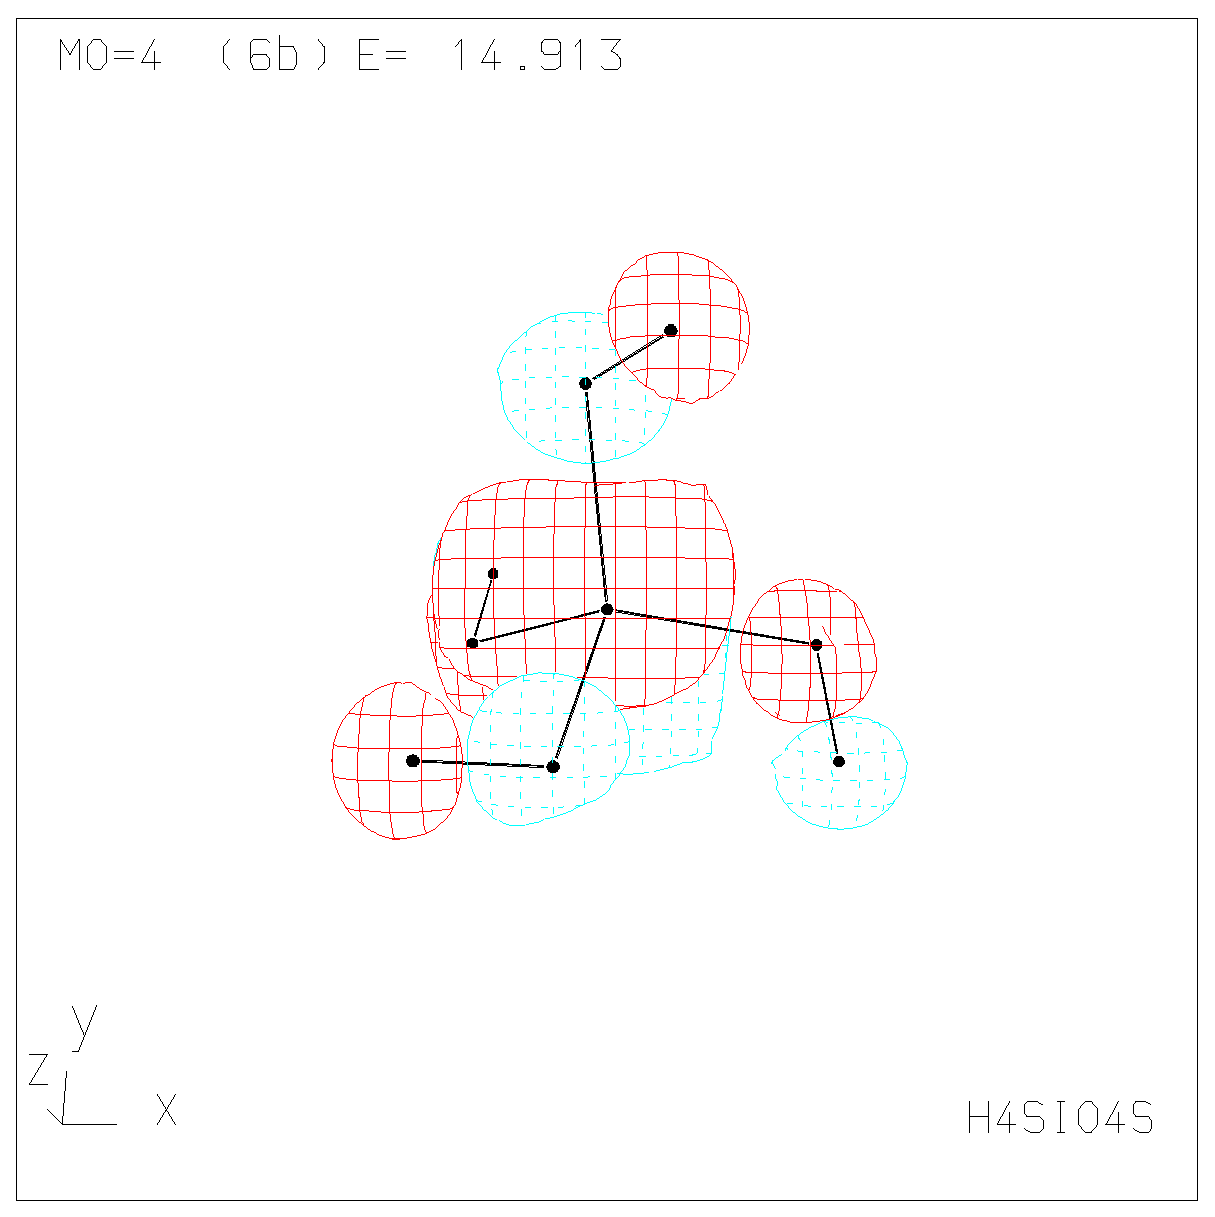
\includegraphics[width=5cm]{h4sio4_obrazky/s2_4.eps} \label{obr_h4sio4_MO_s2_4}}
\subfigure[MO 16]{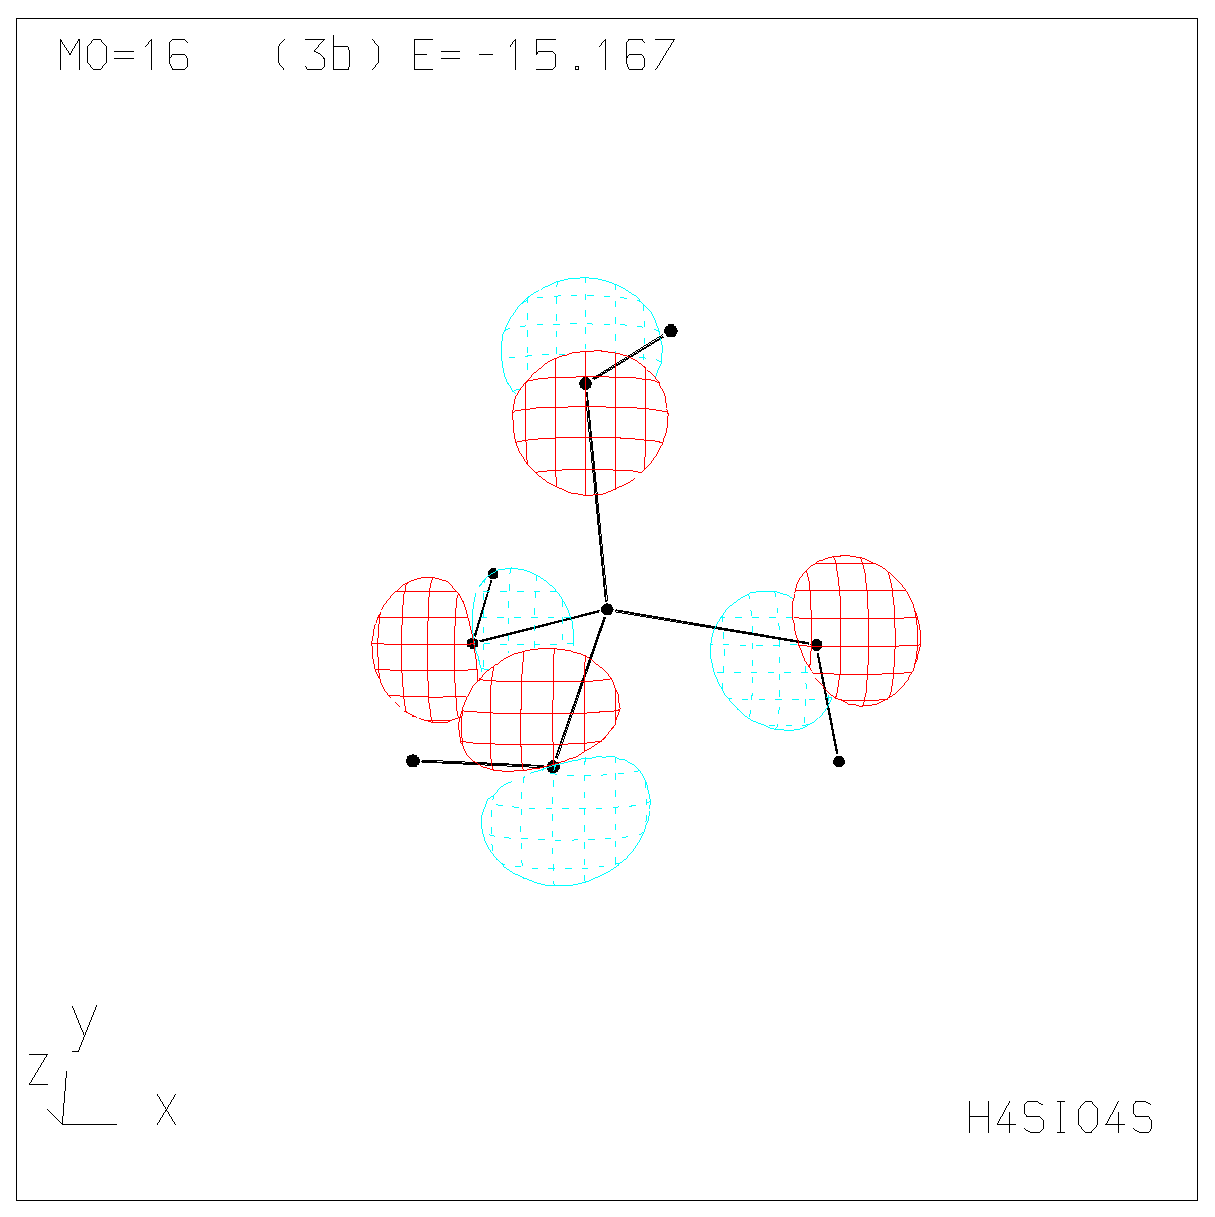
\includegraphics[width=5cm]{h4sio4_obrazky/s2_16.eps}\label{obr_h4sio4_MO_s2_16}}
\subfigure[MO 21]{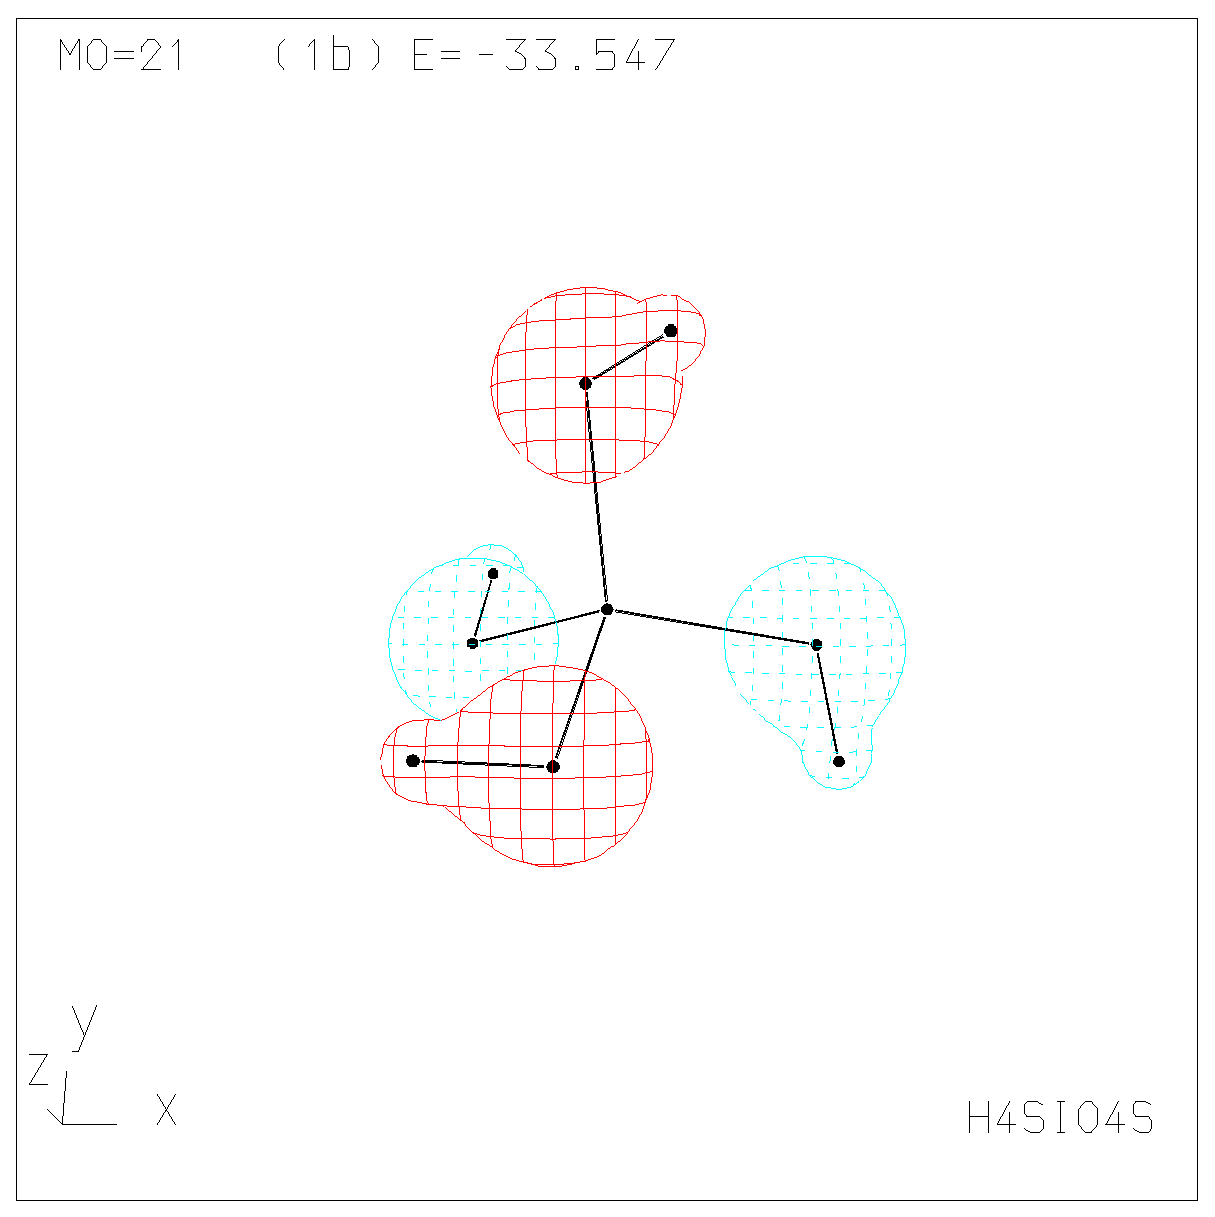
\includegraphics[width=5cm]{h4sio4_obrazky/s2_21.eps}\label{obr_h4sio4_MO_s2_21}}
\caption{Interakce $\bra{11}{\hat{H}}\ket{21}$, $\bra{19}{\hat{H}}\ket{21}$ z~tabulky \ref{tab_h4sio4_vysledky}.}

\label{obr_h4sio4_vysledky_II}\end{center}
\end{figure}

%------------    
 
\begin{figure}
\begin{center}
\subfigure[MO 2]{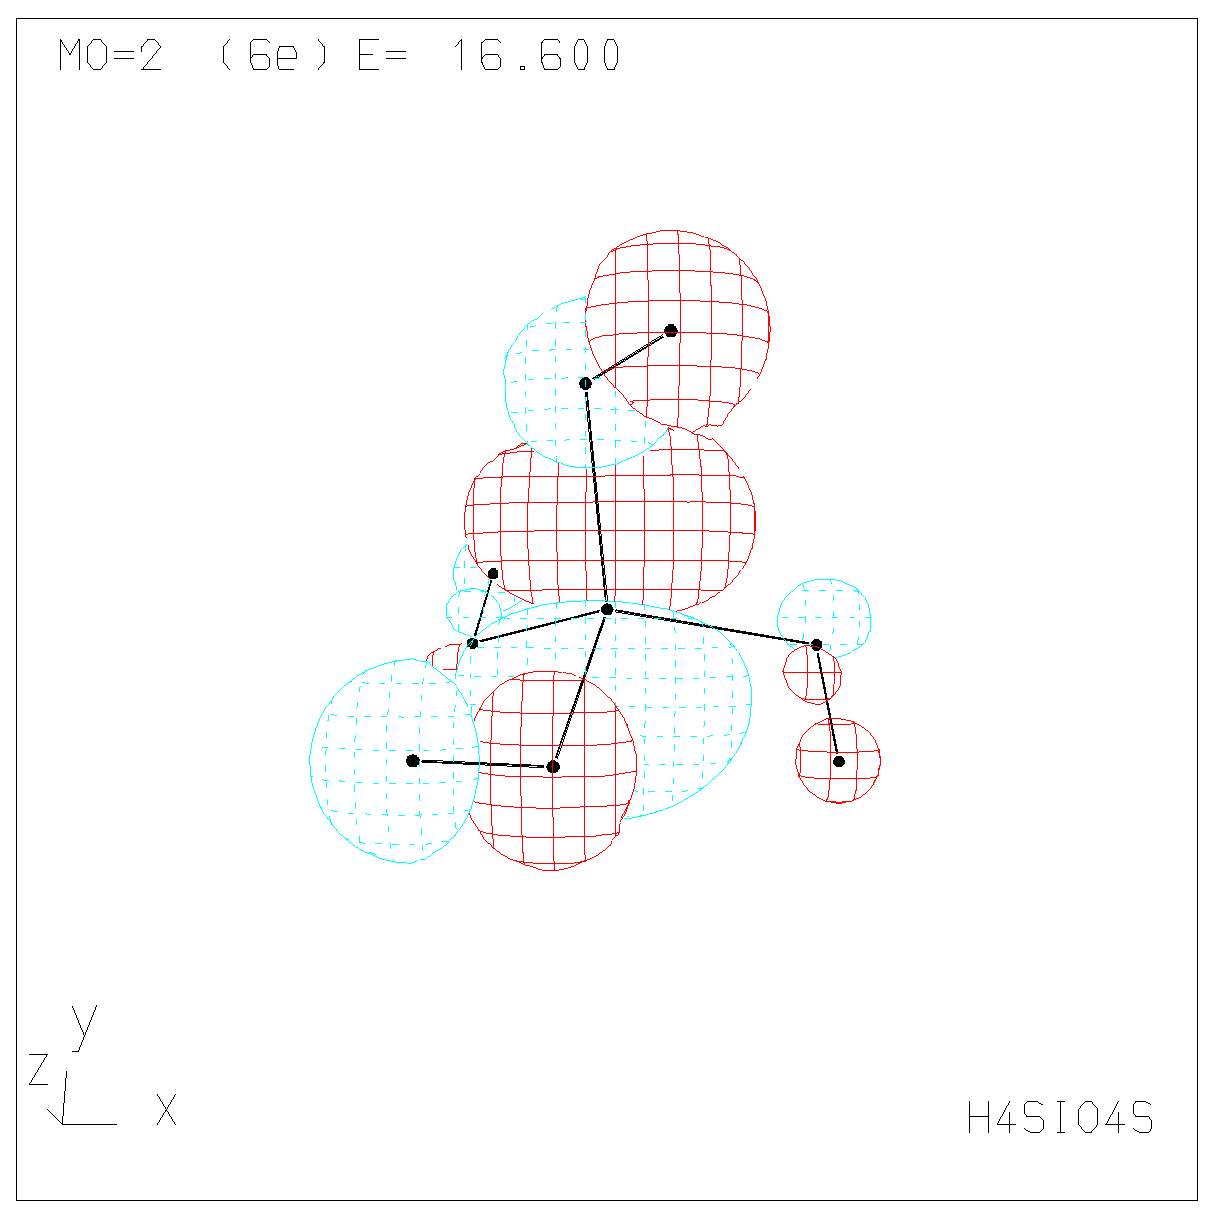
\includegraphics[width=5cm]{h4sio4_obrazky/s3__2.eps} \label{obr_h4sio4_MO_s3_2}}
\subfigure[MO 19]{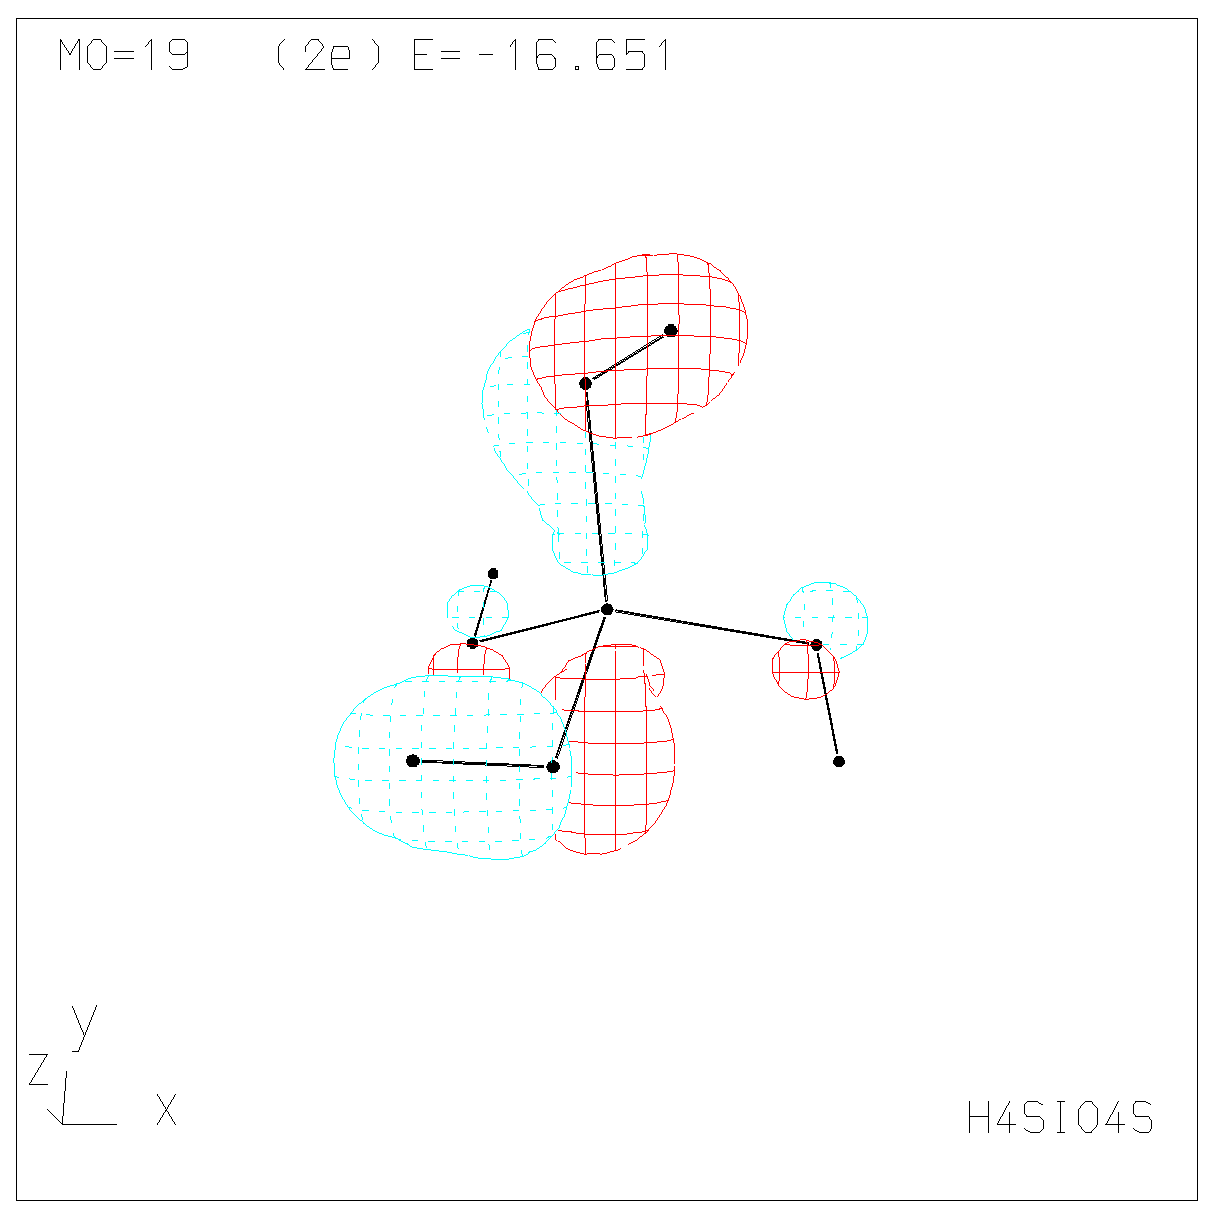
\includegraphics[width=5cm]{h4sio4_obrazky/s3__19.eps}\label{obr_h4sio4_MO_s3_19}}
\subfigure[MO 22]{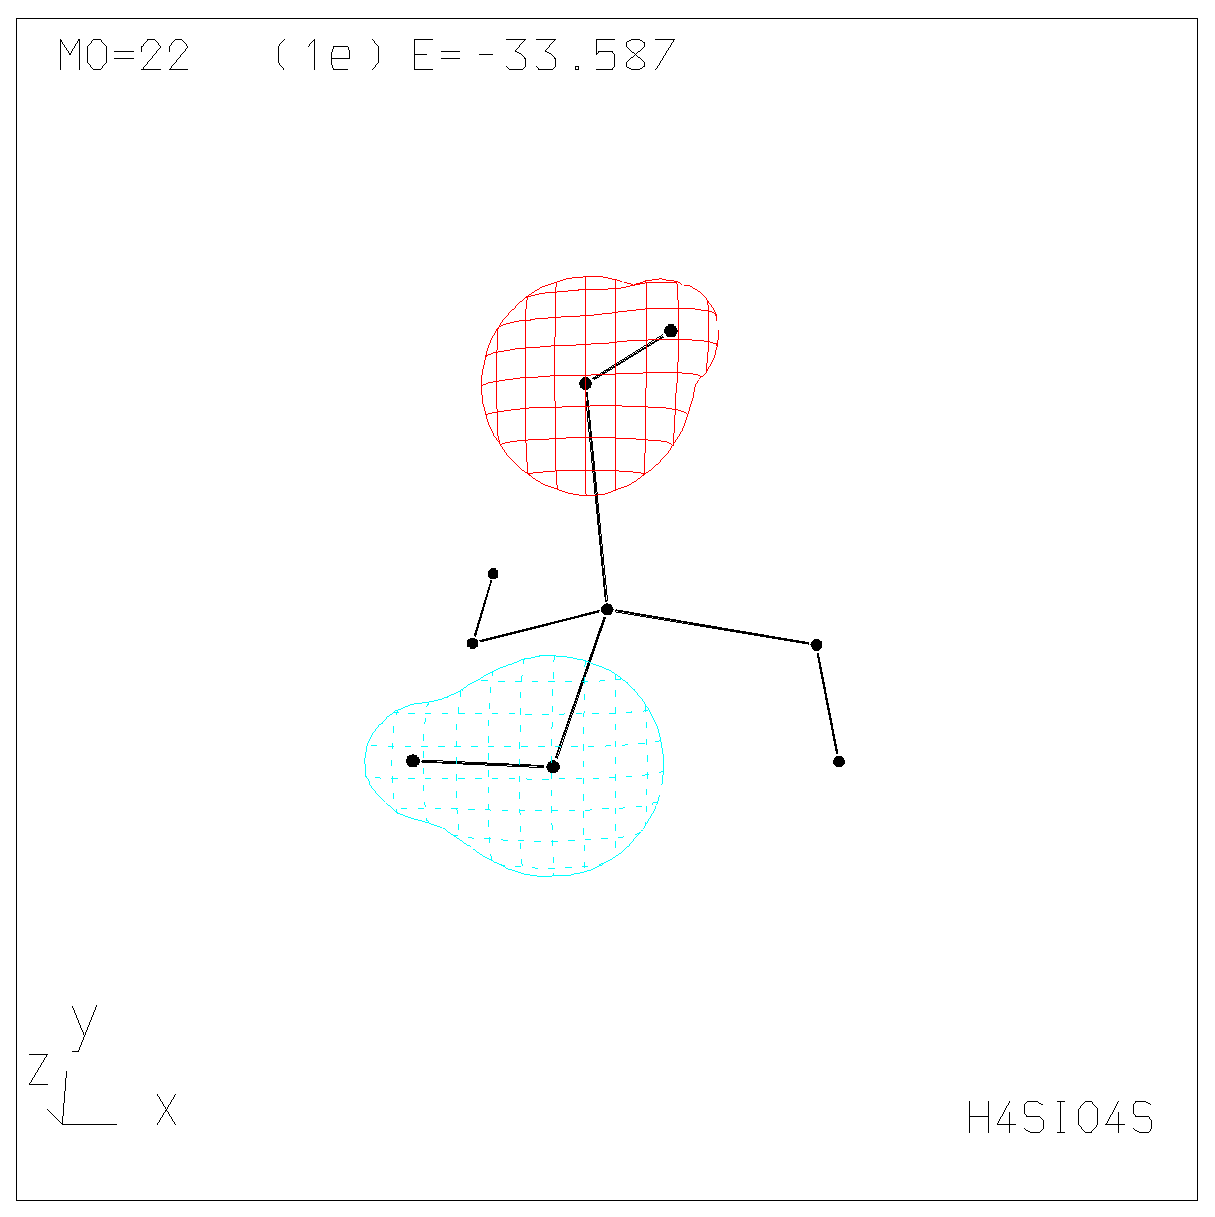
\includegraphics[width=5cm]{h4sio4_obrazky/s3__22.eps}\label{obr_h4sio4_MO_s2_21}}
\caption{Interakce $\bra{15}{\hat{H}}\ket{22}$, $\bra{18}{\hat{H}}\ket{22}$ z~tabulky \ref{tab_h4sio4_vysledky}.}
\label{obr_h4sio4_vysledky_III}
\end{center}
\end{figure} 
%-------------------------------------------------------------------------------------
\subsection{Molekula Si(OH)$_3$CH$_3$}
Molekula \ce{H3SiO3CH3} byla zvolena jako příklad přímé interakce křemík$-$uhlík ve sloučeninách, kde je křemík koordinován čtyřmi atomy. Tato molekula nevykazuje žádnou symetrii. Pro výběr FMO se opět vycházelo ze znalosti interakčního diagramu. 
Fragmentové orbitaly  7, 22 a~26 se navzájem mísí za vzniku MO číslo 3, 11 a~26, znázorněných na obrázku \ref{obr_sioh3ch3_vysledky_I}. Fragmentové orbitaly  21 a~23 se navzájem mísí za vzniku MO číslo 2 a~25, znázorněných na obrázku\ref{obr_sioh3ch3_vysledky_III}. 
Fragmentové orbitaly  7 a~25 se navzájem mísí za vzniku MO číslo 5 a~11, znázorněných na obrázku \ref{obr_sioh3ch3_vysledky_II}.    

\begin{figure}
\begin{center}
\subfigure[Interakční diagram pro \ce{H3SiO3CH3}.]{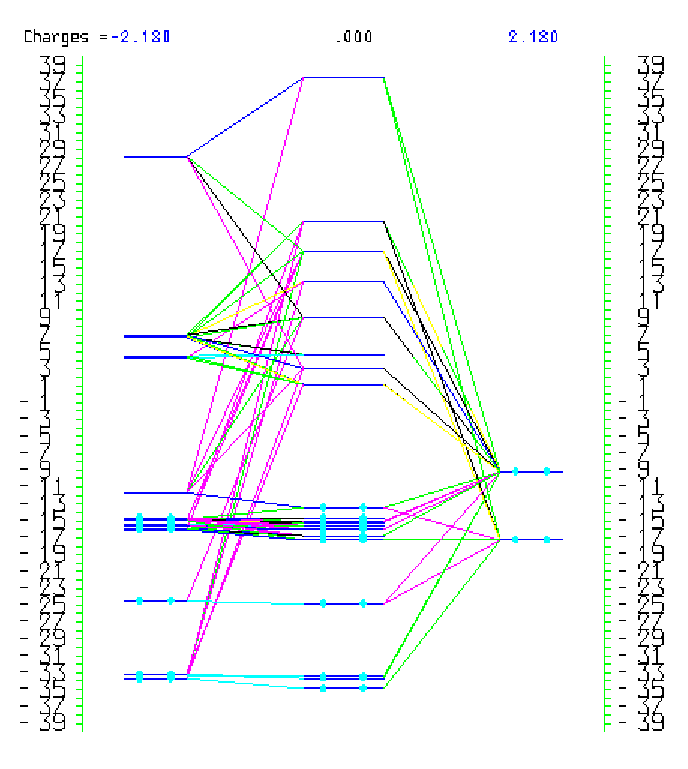
\includegraphics[width=5cm]{sioh3ch3_diagram_upraveny.eps} \label{h4sio4_diagram_upraveny}}
\subfigure[Optimalizovaná struktura \ce{Si(OH)3CH3}.]{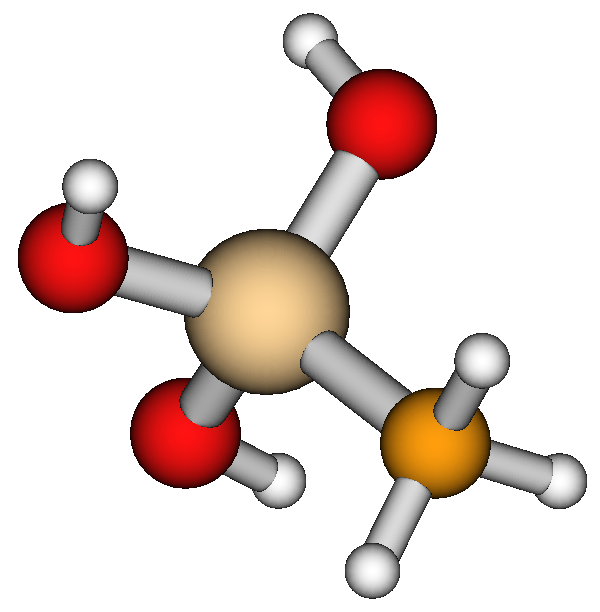
\includegraphics[width=5cm]{si(oh)3ch3_obr.png}\label{obr_sioh3ch3_opt_struktura}}
\label{obr_h4sio4_vysledky_I}
\end{center}
\end{figure}


  
\begin{table}[htbp]
\caption{Výsledné mísení orbitalů pro \ce{Si(OH)3CH3}}
\begin{center}
\begin{tabular}{|r|r|r|r|r|r|r|r|}
\hline
\multicolumn{2}{|c|}{$\bra{22}{\hat{H}}\ket{26}$, $\bra{7}{\hat{H}}\ket{26}$} & \multicolumn{2}{|c|}{$\bra{7}{\hat{H}}\ket{25}$}& \multicolumn{2}{|c|}{$\bra{21}{\hat{H}}\ket{23}$} &\multicolumn{2}{|c|}{$\bra{20}{\hat{H}}\ket{24}$} \\
\hline
\hline
\multicolumn{1}{|l|}{MO} & \multicolumn{1}{r|}{W} & \multicolumn{1}{l|}{MO} & \multicolumn{1}{r|}{W} & MO & \multicolumn{1}{r|}{W}& MO & \multicolumn{1}{r|}{W} \\ \hline
3 & 46 \% & 11 & 79 \% &25 & 100 \%& 24 & 100 \% \\ \hline
11 & 71 \% & 5 & 40 \% & 2 & 34 \% &4 & 58 \% \\ \hline
26 & 98 \% & - & - &  -& - &-&- \\ \hline
\end{tabular}
\end{center}
\label{tab_sioh3ch3_vysledky}
\end{table}

\begin{figure}
\begin{center}
\subfigure[MO 3]{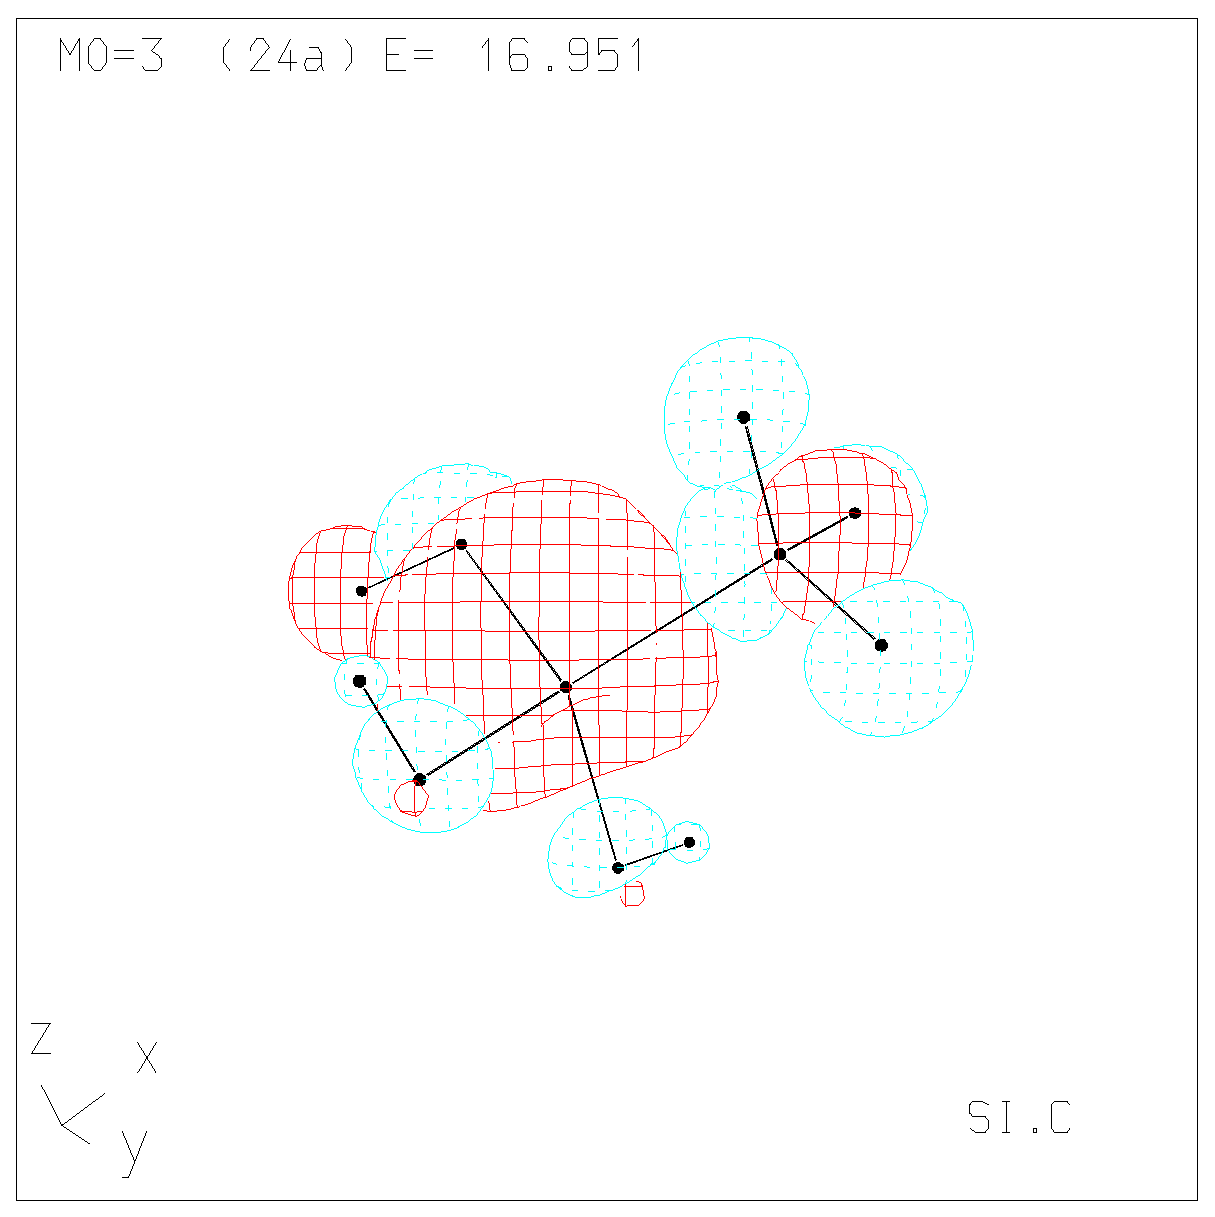
\includegraphics[width=5cm]{sioh3ch3_obrazky/s1_3.eps} \label{obr_sioh3ch3_MO_s1_3}}
\subfigure[MO 11]{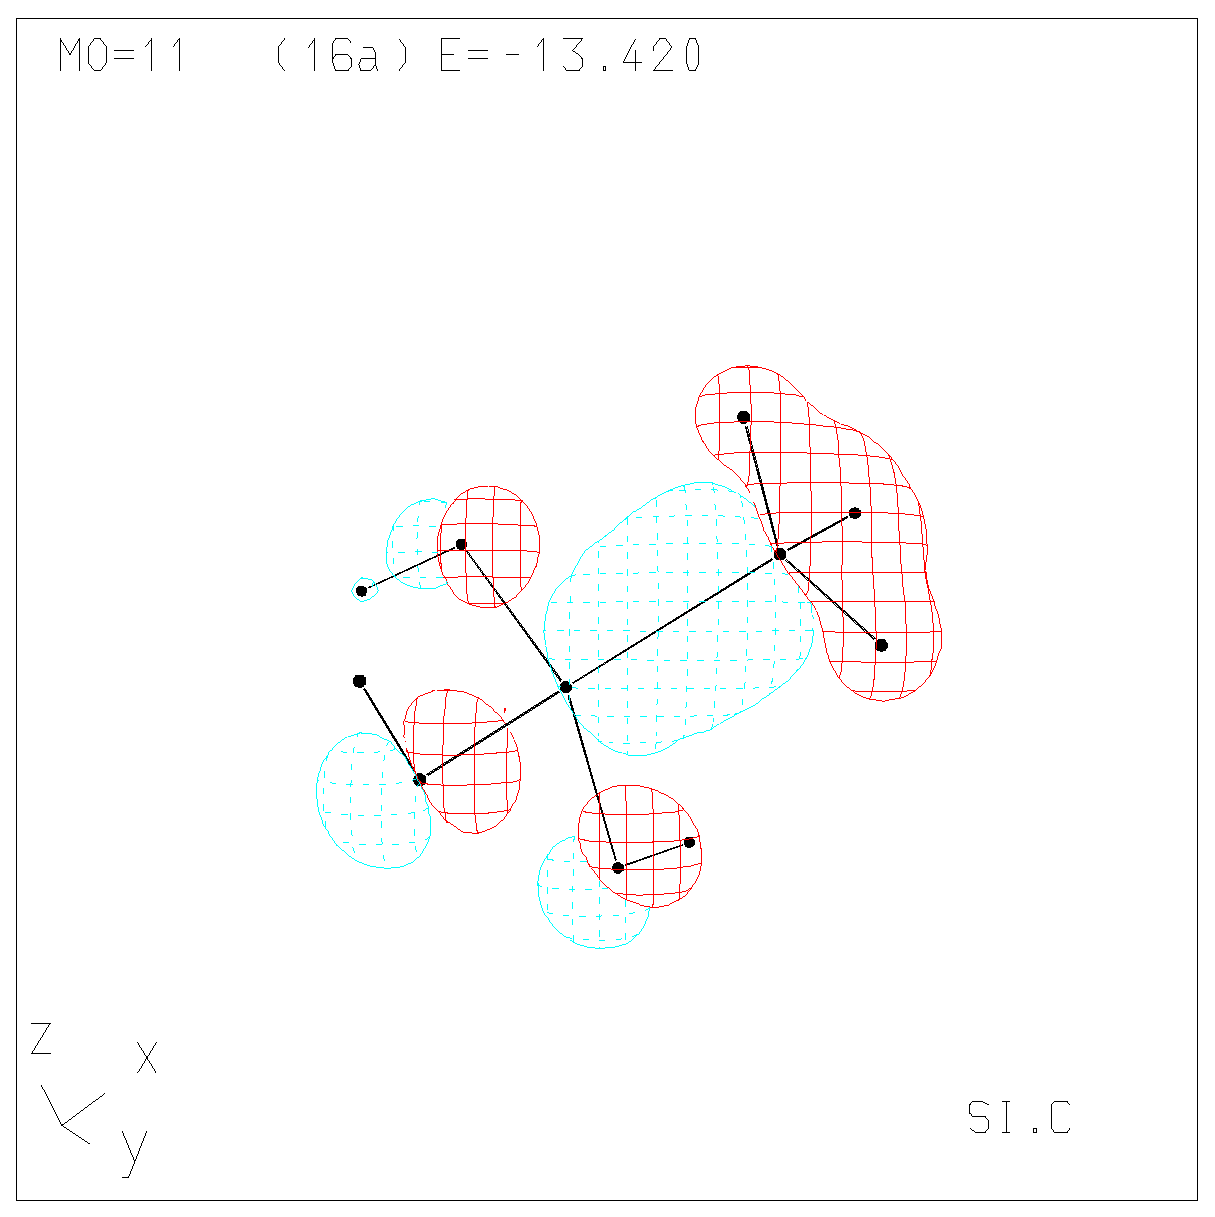
\includegraphics[width=5cm]{sioh3ch3_obrazky/s1_11.eps}\label{obr_sioh3ch3_MO_s1_11}}
\subfigure[MO 26]{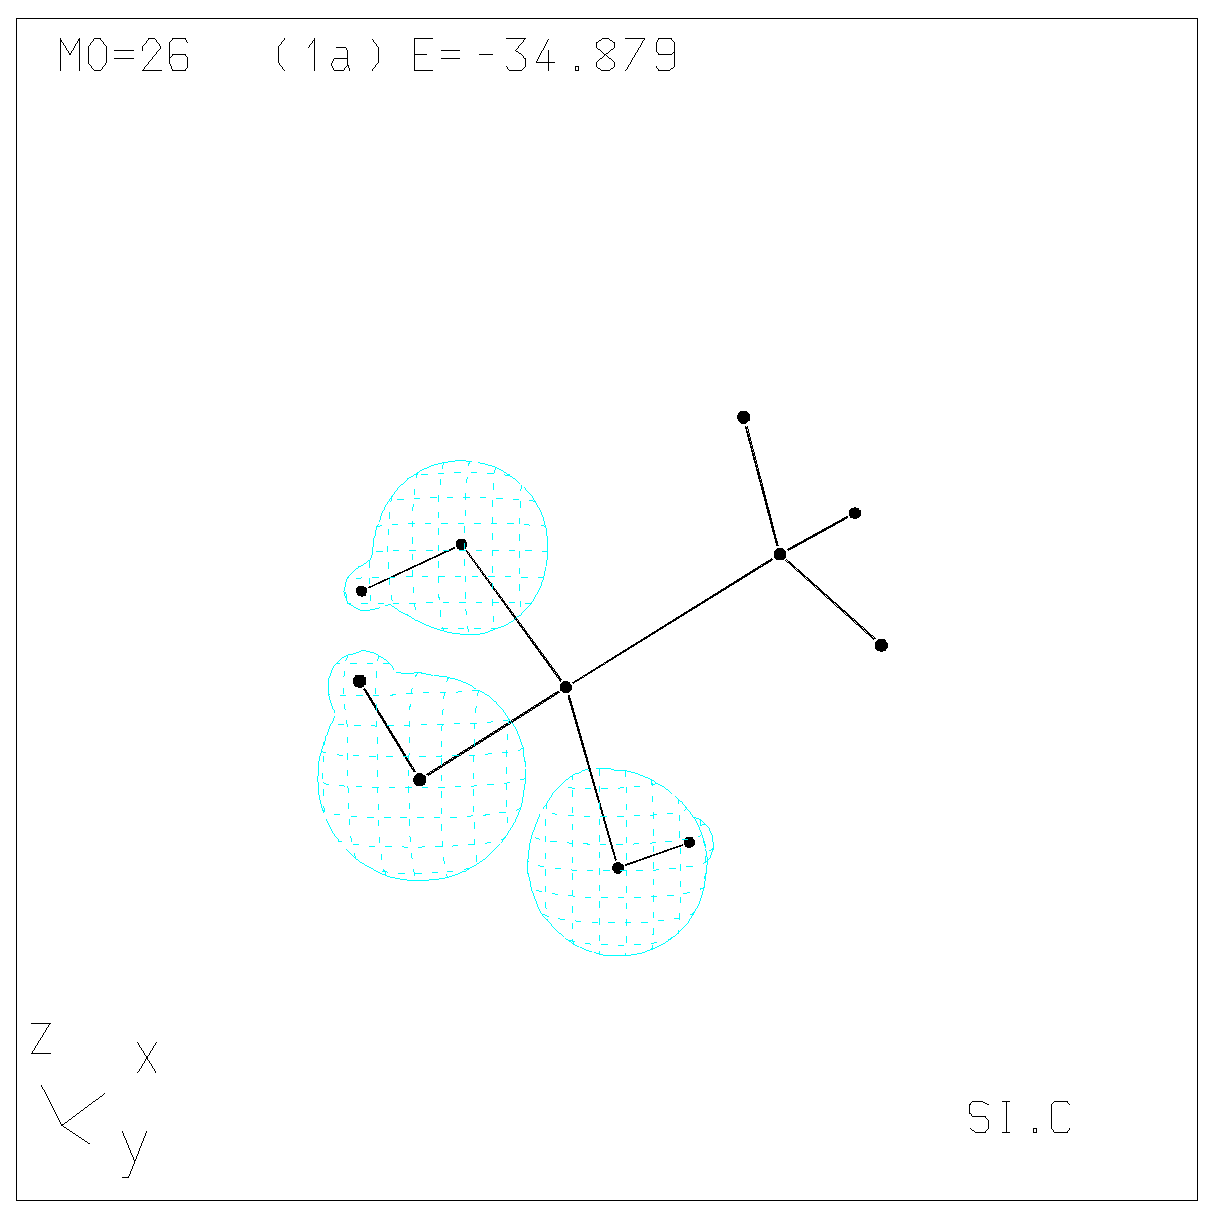
\includegraphics[width=5cm]{sioh3ch3_obrazky/s1_26.eps}\label{obr_sioh3ch3_MO_s1_26}}
\caption{Interakce $\bra{22}{\hat{H}}\ket{26}$, $\bra{7}{\hat{H}}\ket{26}$  z~tabulky \ref{tab_sioh3ch3_vysledky}.}

\label{obr_sioh3ch3_vysledky_I}\end{center}
\end{figure} 
  
\begin{figure}
\begin{center}
\subfigure[MO 5]{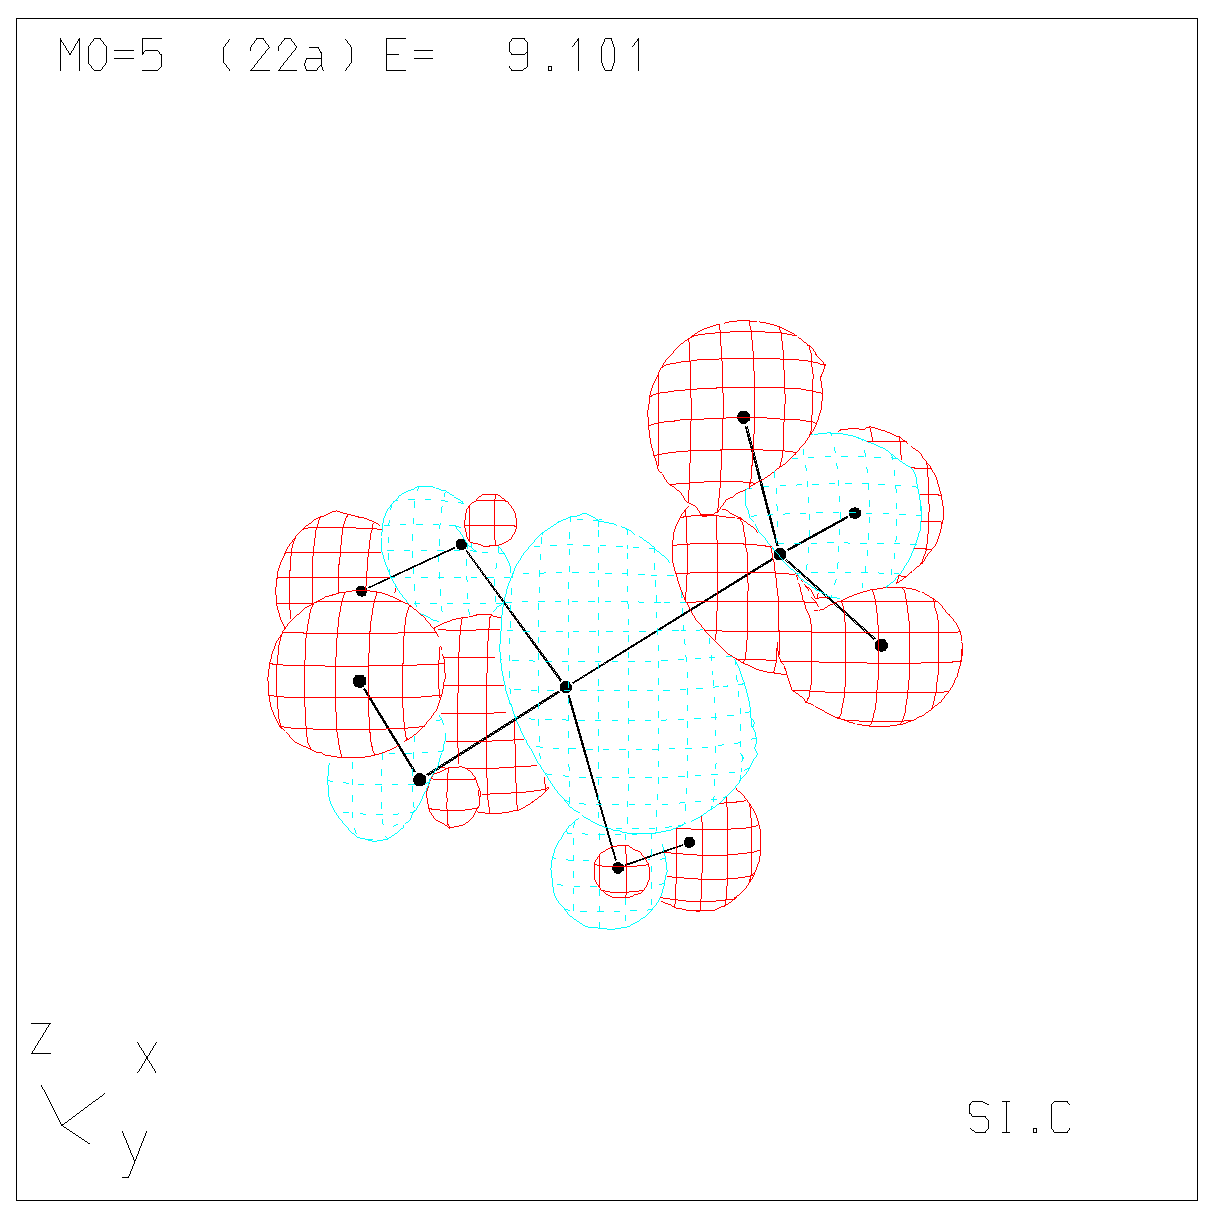
\includegraphics[width=5cm]{sioh3ch3_obrazky/s2_5.eps} \label{obr_sioh3ch3_MO_s2_5}}
\subfigure[MO 11]{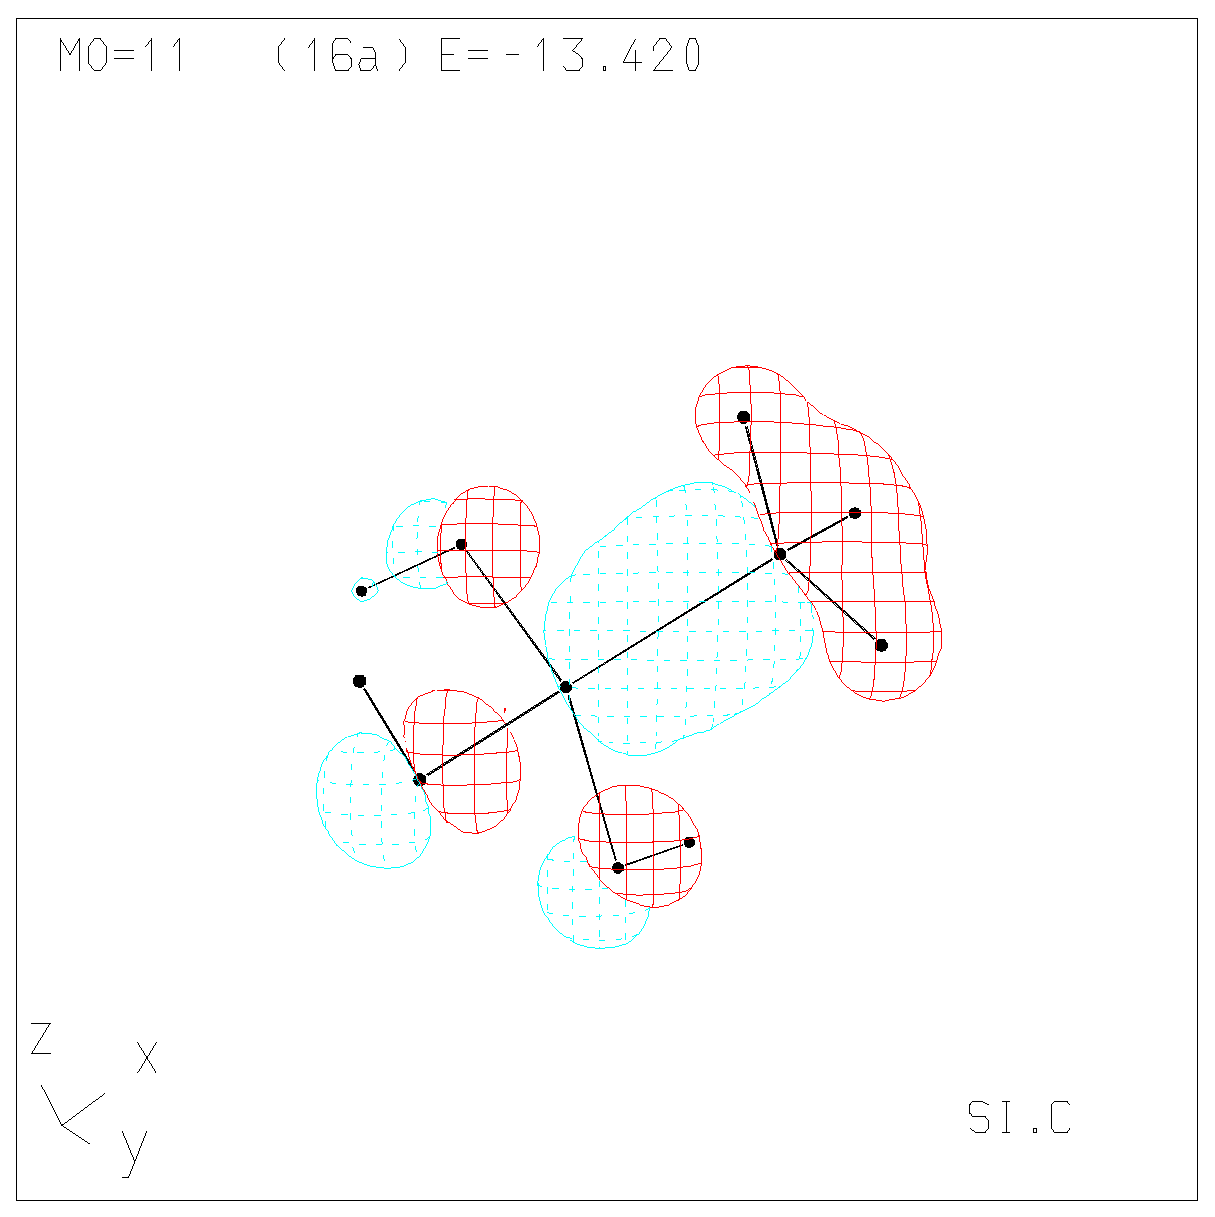
\includegraphics[width=5cm]{sioh3ch3_obrazky/s2_11.eps}\label{obr_sioh3ch3_MO_s2_11}}
\caption{Interakce $\bra{7}{\hat{H}}\ket{25}$ z~tabulky \ref{tab_sioh3ch3_vysledky}.}

\label{obr_sioh3ch3_vysledky_II}\end{center}
\end{figure} 

 \clearpage
 
\begin{figure}
\begin{center}
\subfigure[MO 5]{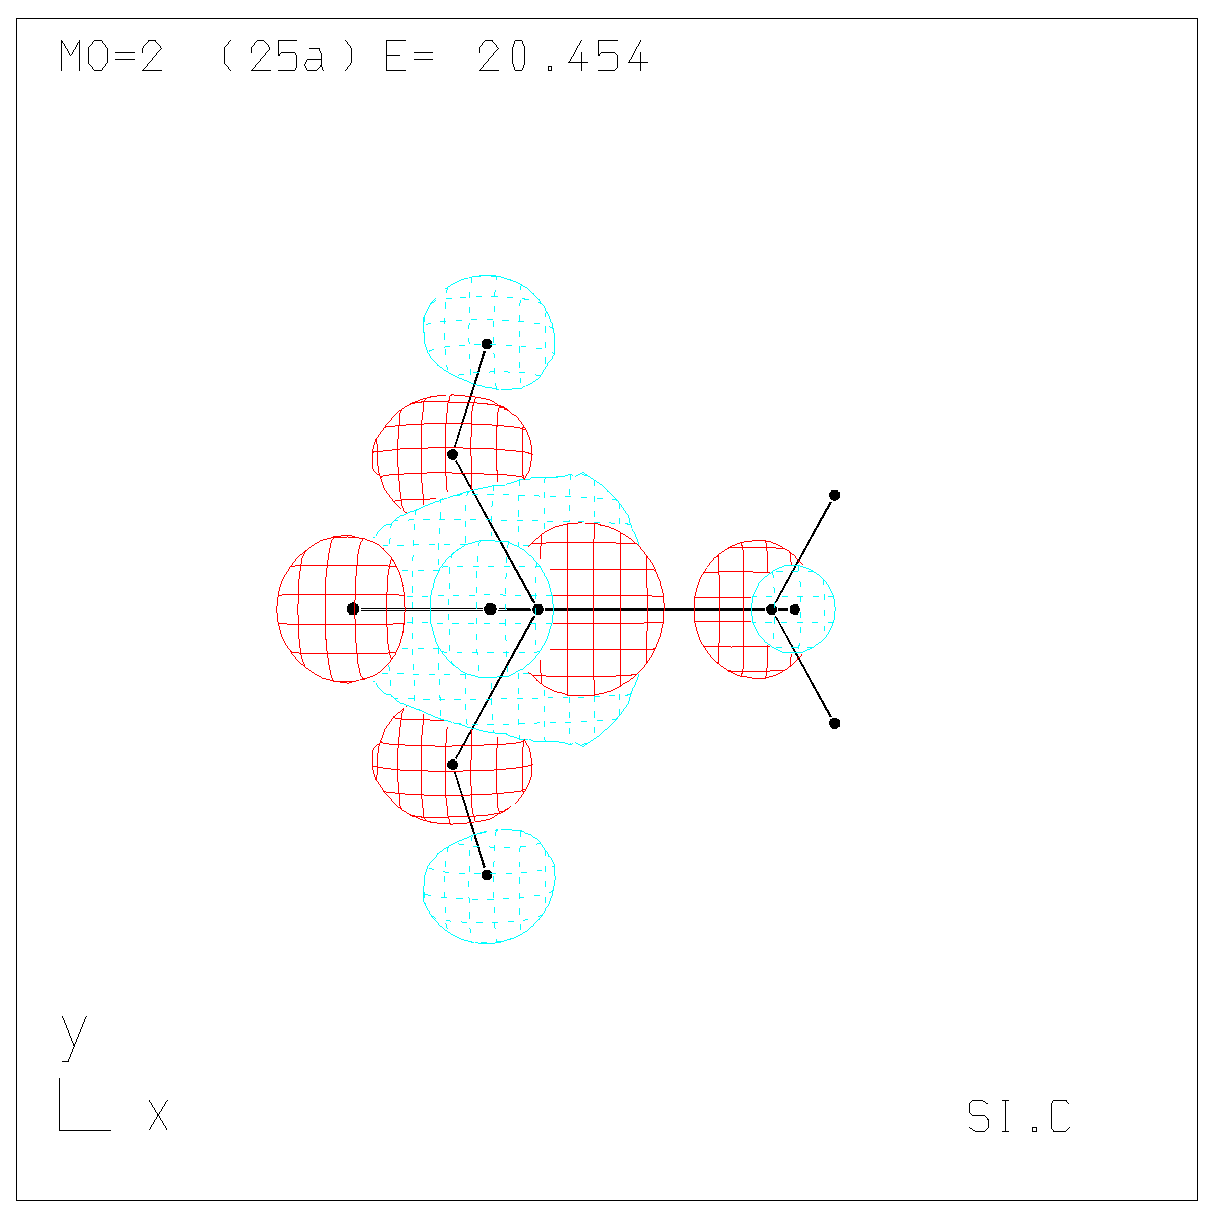
\includegraphics[width=5cm]{sioh3ch3_obrazky/s3_2.eps} \label{obr_sioh3ch3_MO_s3_2}}
\subfigure[MO 11]{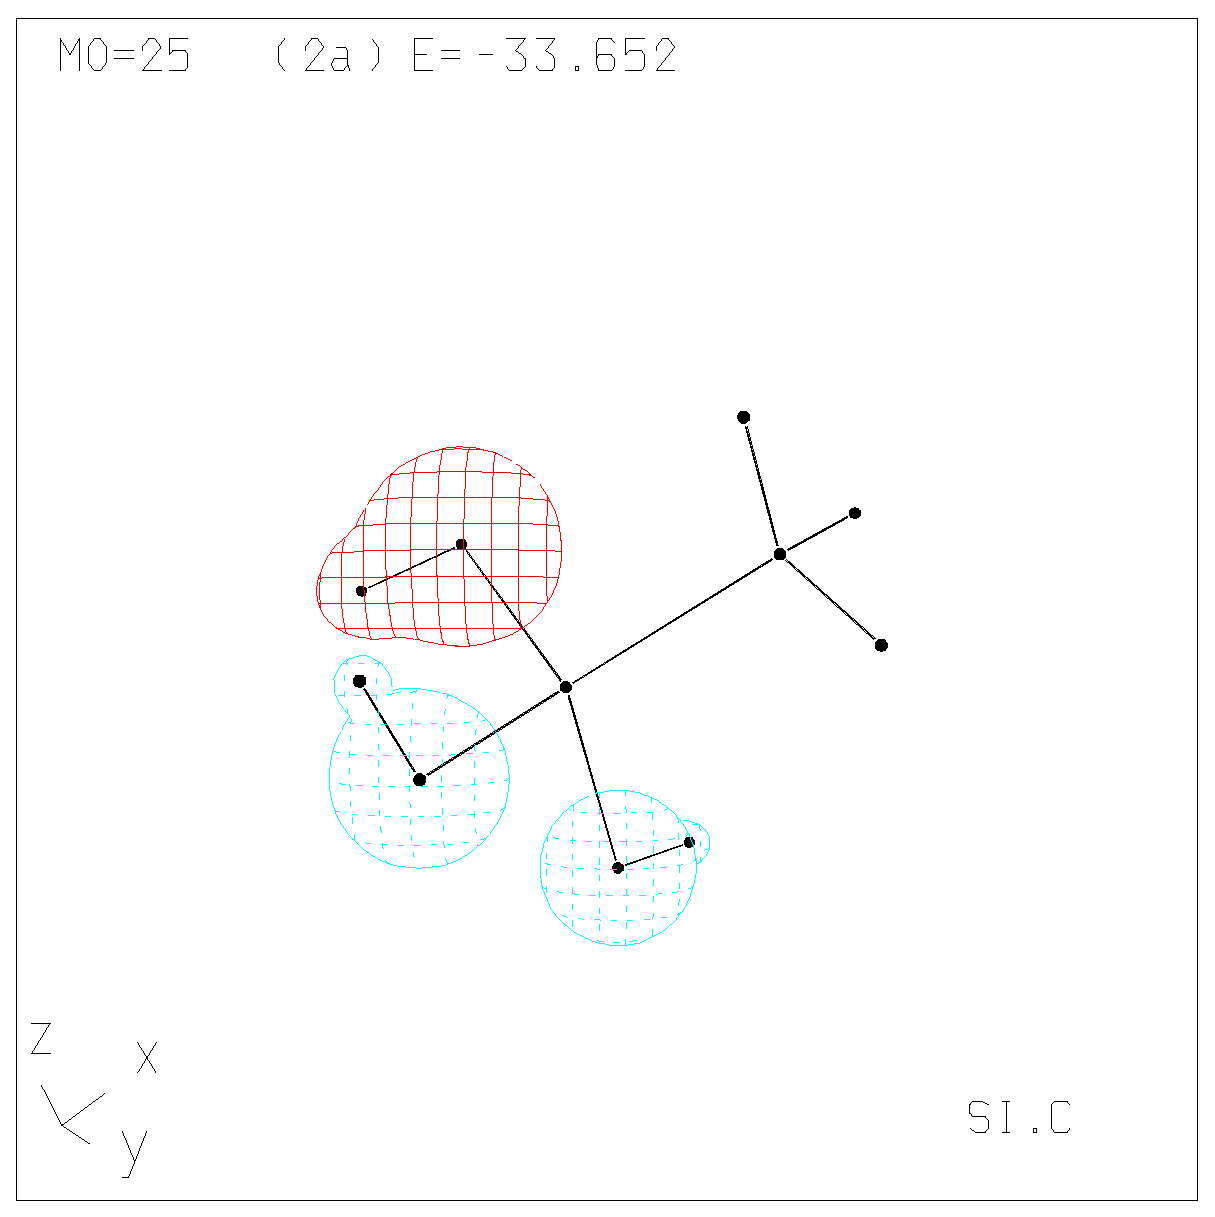
\includegraphics[width=5cm]{sioh3ch3_obrazky/s3_25.eps}\label{obr_sioh3ch3_MO_s3_25}}
\caption{Interakce $\bra{21}{\hat{H}}\ket{23}$  z~tabulky \ref{tab_sioh3ch3_vysledky}.}

\label{obr_sioh3ch3_vysledky_III}\end{center}
\end{figure} 
   
Fragmentové orbitaly  20 a~24 se navzájem mísí za vzniku MO číslo 4 a~24, znázorněných na obrázku \ref{obr_sioh3ch3_vysledky_IV}.   
\begin{figure}
\begin{center}
\subfigure[MO 5]{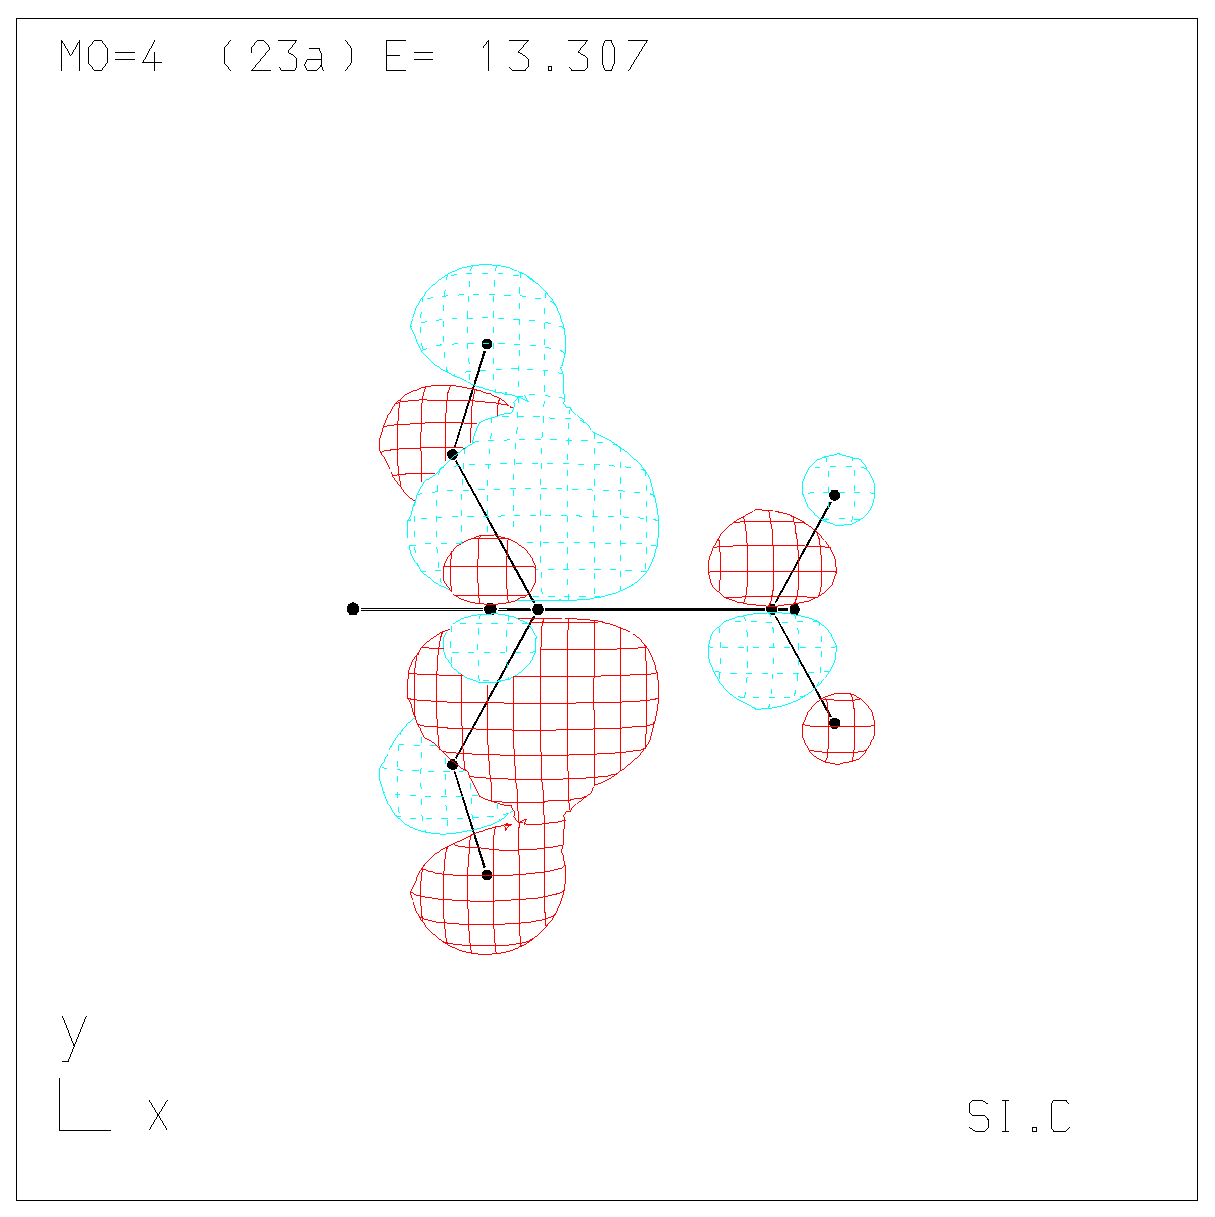
\includegraphics[width=5cm]{sioh3ch3_obrazky/s4_4.eps} \label{obr_sioh3ch3_MO_s4_4}}
\subfigure[MO 11]{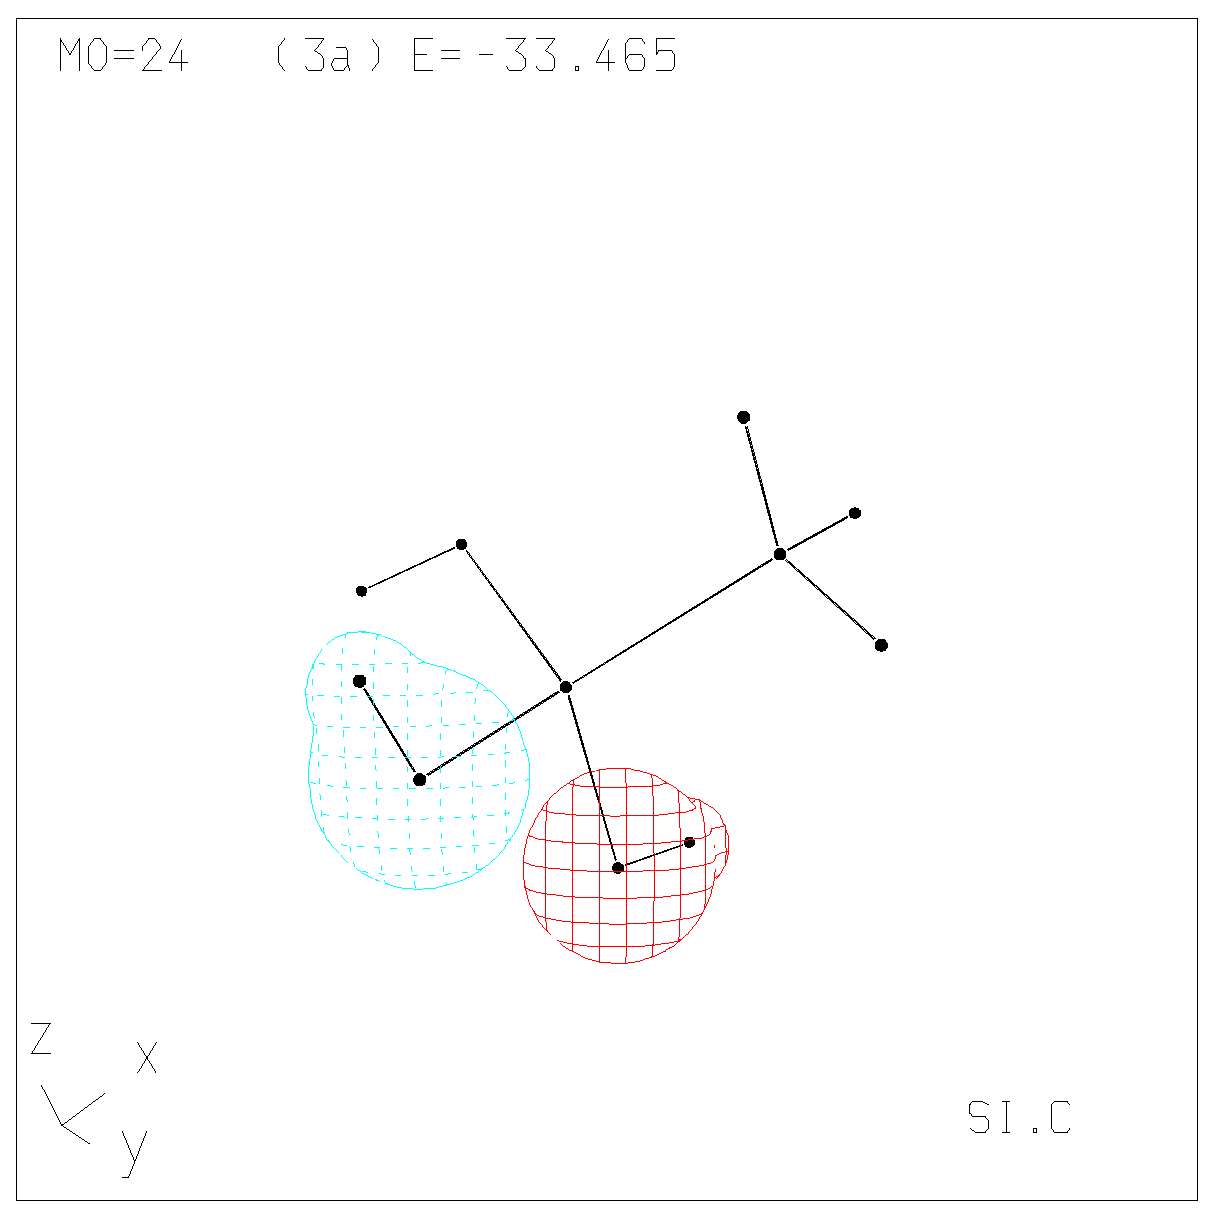
\includegraphics[width=5cm]{sioh3ch3_obrazky/s4_24.eps}\label{obr_sioh3ch3_MO_s4_24}}
\caption{Interakce $\bra{20}{\hat{H}}\ket{24}$  z~tabulky \ref{tab_sioh3ch3_vysledky}.}

\label{obr_sioh3ch3_vysledky_IV}\end{center}
\end{figure} 
 %-------------------------------------------------------------------------------------------- 
  \subsection{Molekula (H$_6$SiO$_6$)$^{2-}$}
  Molekula \ce{(H6SiO6)^{2-}} představuje příklad křemíku koordinovaného šesti kyslíky. Molekula vykazovala vysokou symetrii S$_6$, pro výpočet byla z~důvodu technických problémů s~programem C.A.C.A.O. použita symetrie C$_i$. Tato molekula je hypervalentní a~celkový náboj je $2-$. Fragmentové orbitaly  24, 30 a~34 se navzájem mísí za vzniku MO číslo 1, 28 a~34 znázorněných na obrázku \ref{obr_h6sio6_vysledky_I}. Fragmentové orbitaly  21, 28 a~32 se navzájem mísí za vzniku MO číslo 3, 26 a~32 znázorněných na obrázku \ref{obr_h6sio6_vysledky_II}. Fragmentové orbitaly  22 a~33 se navzájem mísí za vzniku MO číslo 2 znázorněného na obrázku \ref{obr_h6sio6_vysledky_III}. 
  
  \begin{figure}
\begin{center}
\subfigure[Interakční diagram pro \ce{(H6SiO6)^{2-}}.]{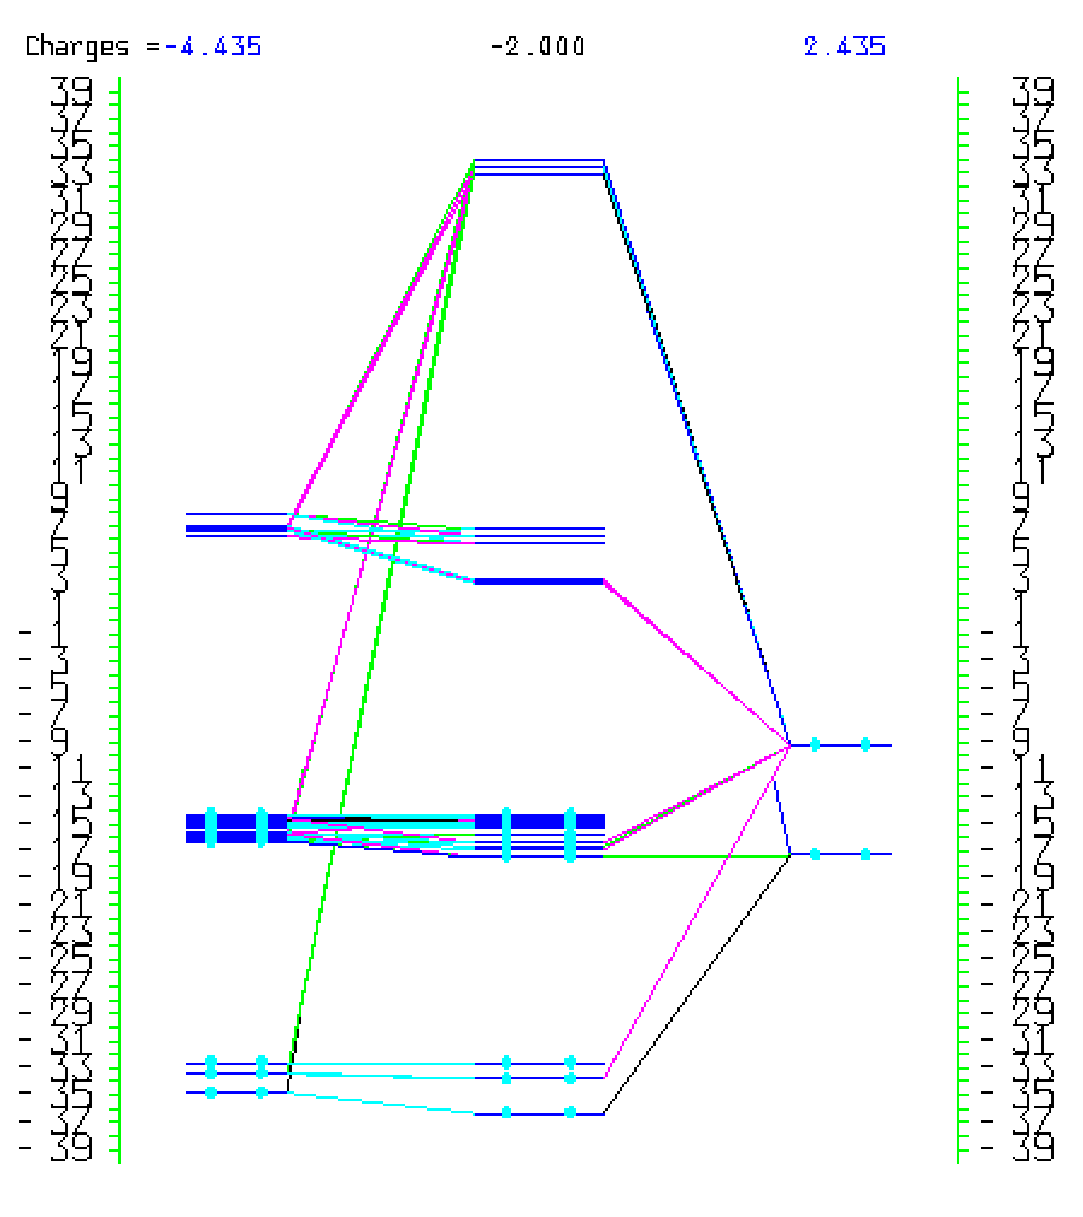
\includegraphics[width=5cm]{h6sio6_diagram.eps} \label{h6sio6_diagram_upraveny}}
\subfigure[Optimalizovaná struktura \ce{(H6SiO6)^{2-}}.]{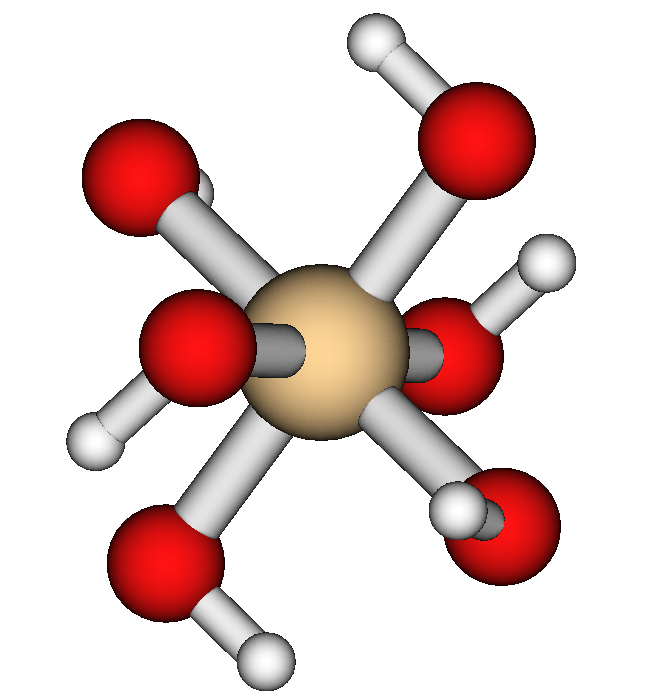
\includegraphics[width=5cm]{obr_h6sio6.png}\label{obr_h6sio6_opt_struktura}}
\label{obr_h6sio6_vysledky_I}
\end{center}
\end{figure}
  
  \begin{table}[htbp]
\caption{Výsledné mísení orbitalů pro \ce{(H6SiO6)^-2}}
\begin{center}
\begin{tabular}{|r|r|r|r|r|r|}
\hline
\multicolumn{2}{|c}{$\bra{30}{\hat{H}}\ket{34}$, $\bra{24}{\hat{H}}\ket{34}$} & \multicolumn{2}{|c|}{$\bra{21}{\hat{H}}\ket{32}$, $\bra{28}{\hat{H}}\ket{32}$}& \multicolumn{2}{|c|}{$\bra{22}{\hat{H}}\ket{33}$} \\
\hline \hline
\multicolumn{1}{|l|}{MO} & \multicolumn{1}{r|}{W} & \multicolumn{1}{l|}{MO} & \multicolumn{1}{r|}{W} & MO & \multicolumn{1}{r|}{W} \\ \hline
1 & 96 \% & 3 & 86 \% &2 & 65 \% \\ \hline
28 & 84 \% & 26 & 97 \% & - & - \\ \hline
34 & 100 \% & 32 & 99 \% &  -& - \\ \hline
\end{tabular}
\label{tab_h6sio6_vysledky}\end{center}
\end{table}
     
\begin{figure}
\begin{center}
\subfigure[MO 5]{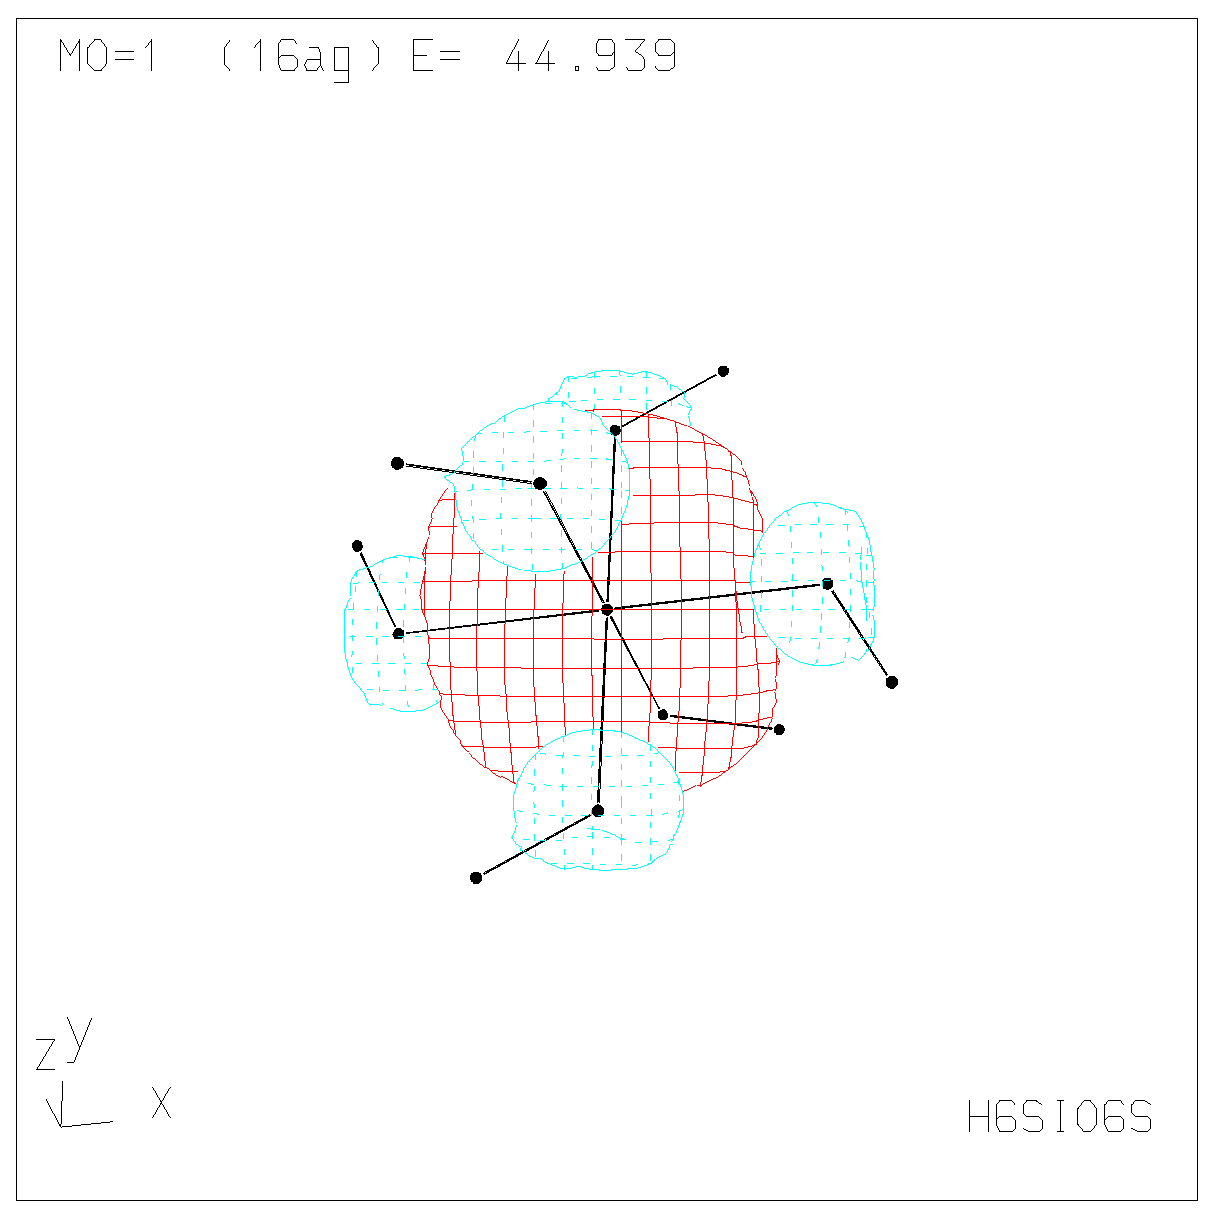
\includegraphics[width=5cm]{h6sio6_obrazky/s1_1.eps} 
\label{obr_h6sio6_MO_s1_1}}
\subfigure[MO 11]{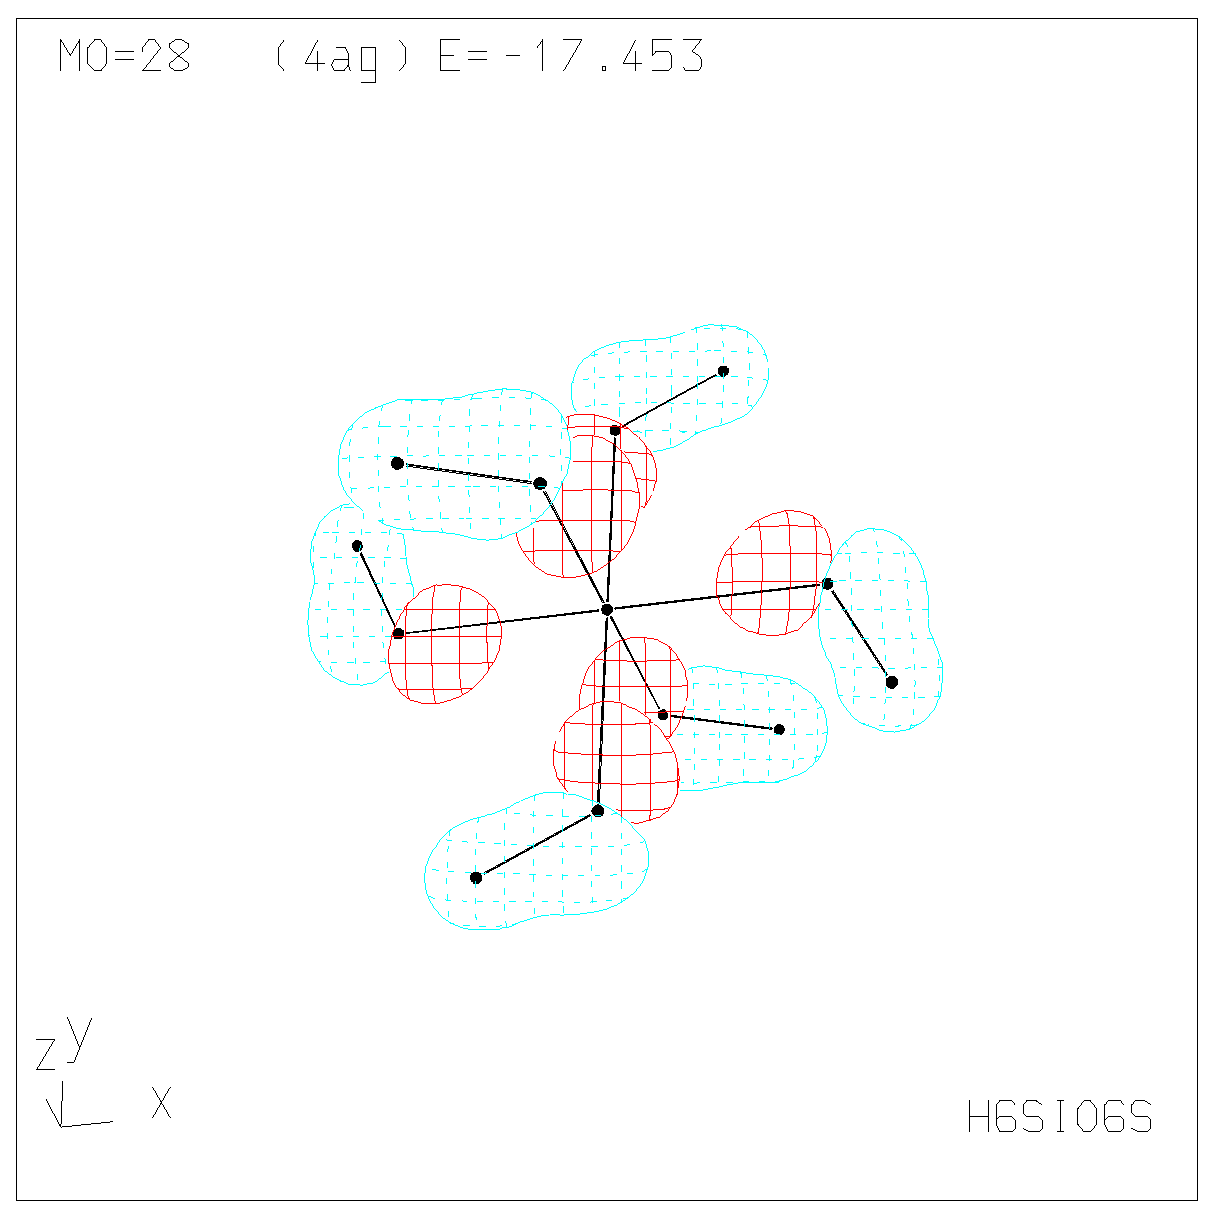
\includegraphics[width=5cm]{h6sio6_obrazky/s1_28.eps}\label{obr_h6sio6_MO_s1_28}}
\subfigure[MO 5]{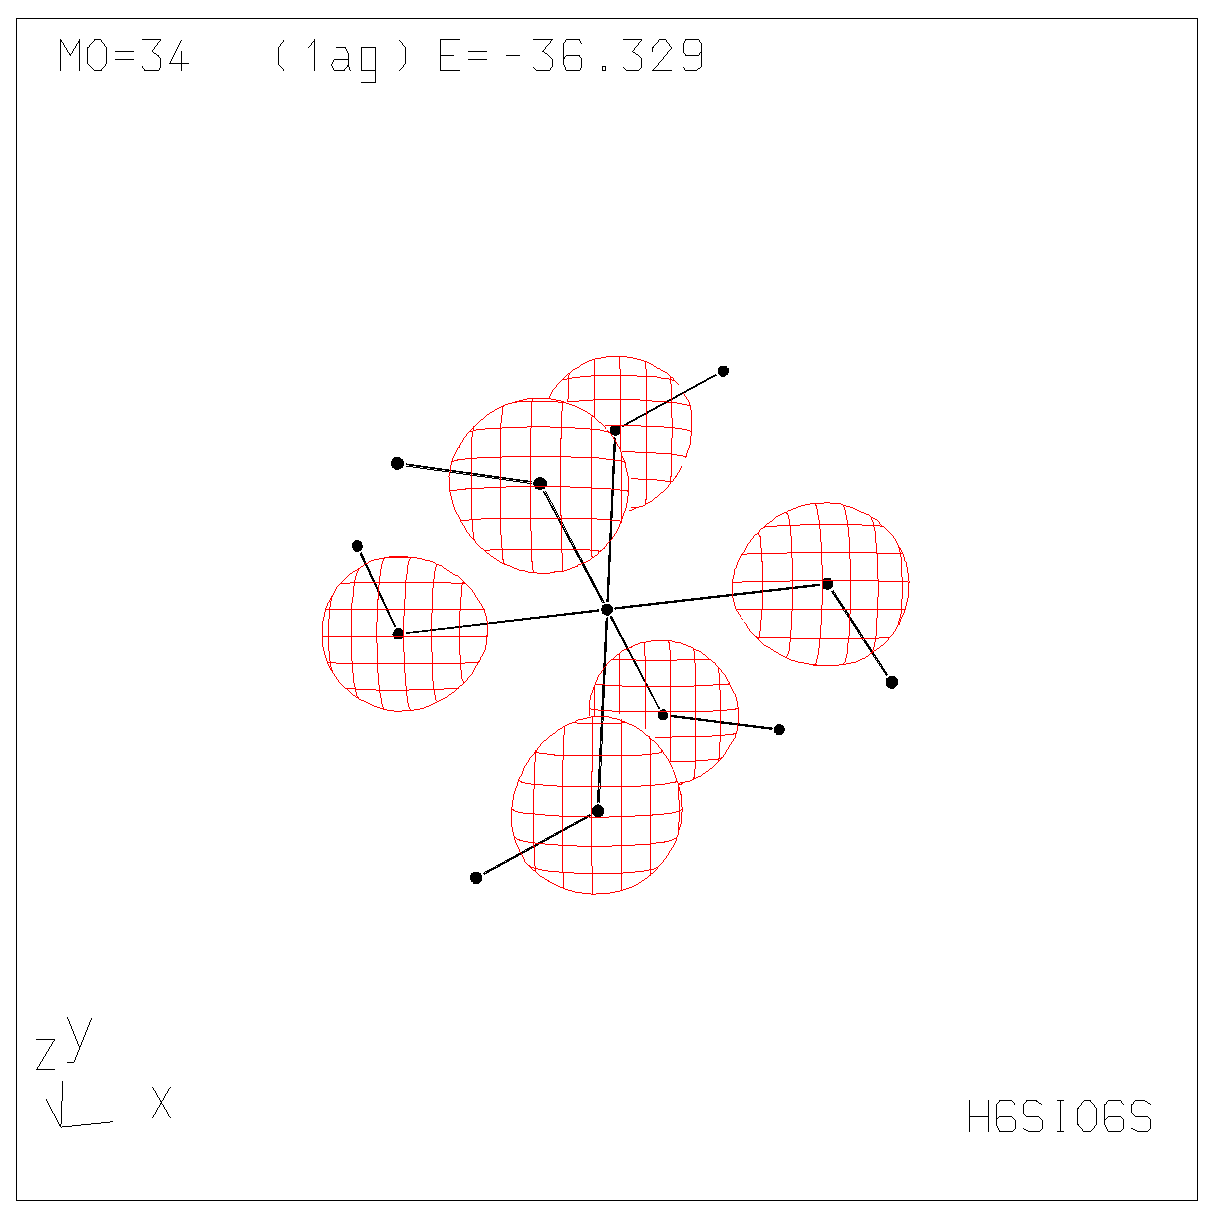
\includegraphics[width=5cm]{h6sio6_obrazky/s1_34.eps} \label{obr_h6sio6_MO_s1_34}}
\caption{Interakce $\bra{30}{\hat{H}}\ket{34}$, $\bra{24}{\hat{H}}\ket{34}$  z~tabulky \ref{tab_h6sio6_vysledky}.}

\label{obr_h6sio6_vysledky_I}\end{center}
\end{figure} 

   
\begin{figure}
\begin{center}
\subfigure[MO 3]{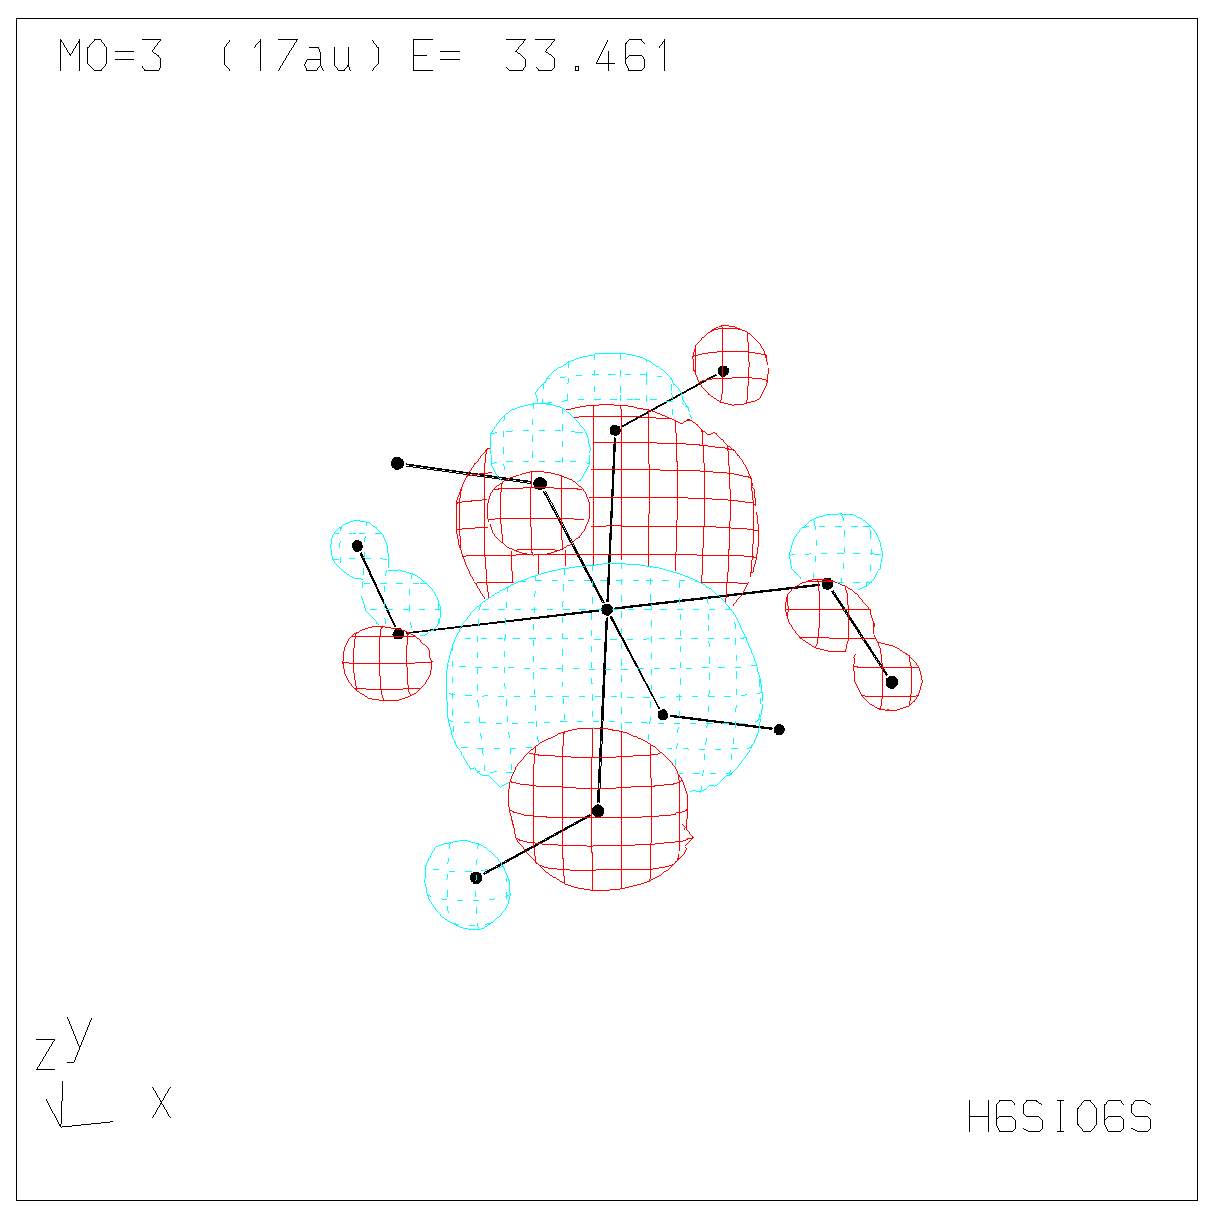
\includegraphics[width=5cm]{h6sio6_obrazky/s2_3.eps} 
\label{obr_h6sio6_MO_s2_3}}
\subfigure[MO 26]{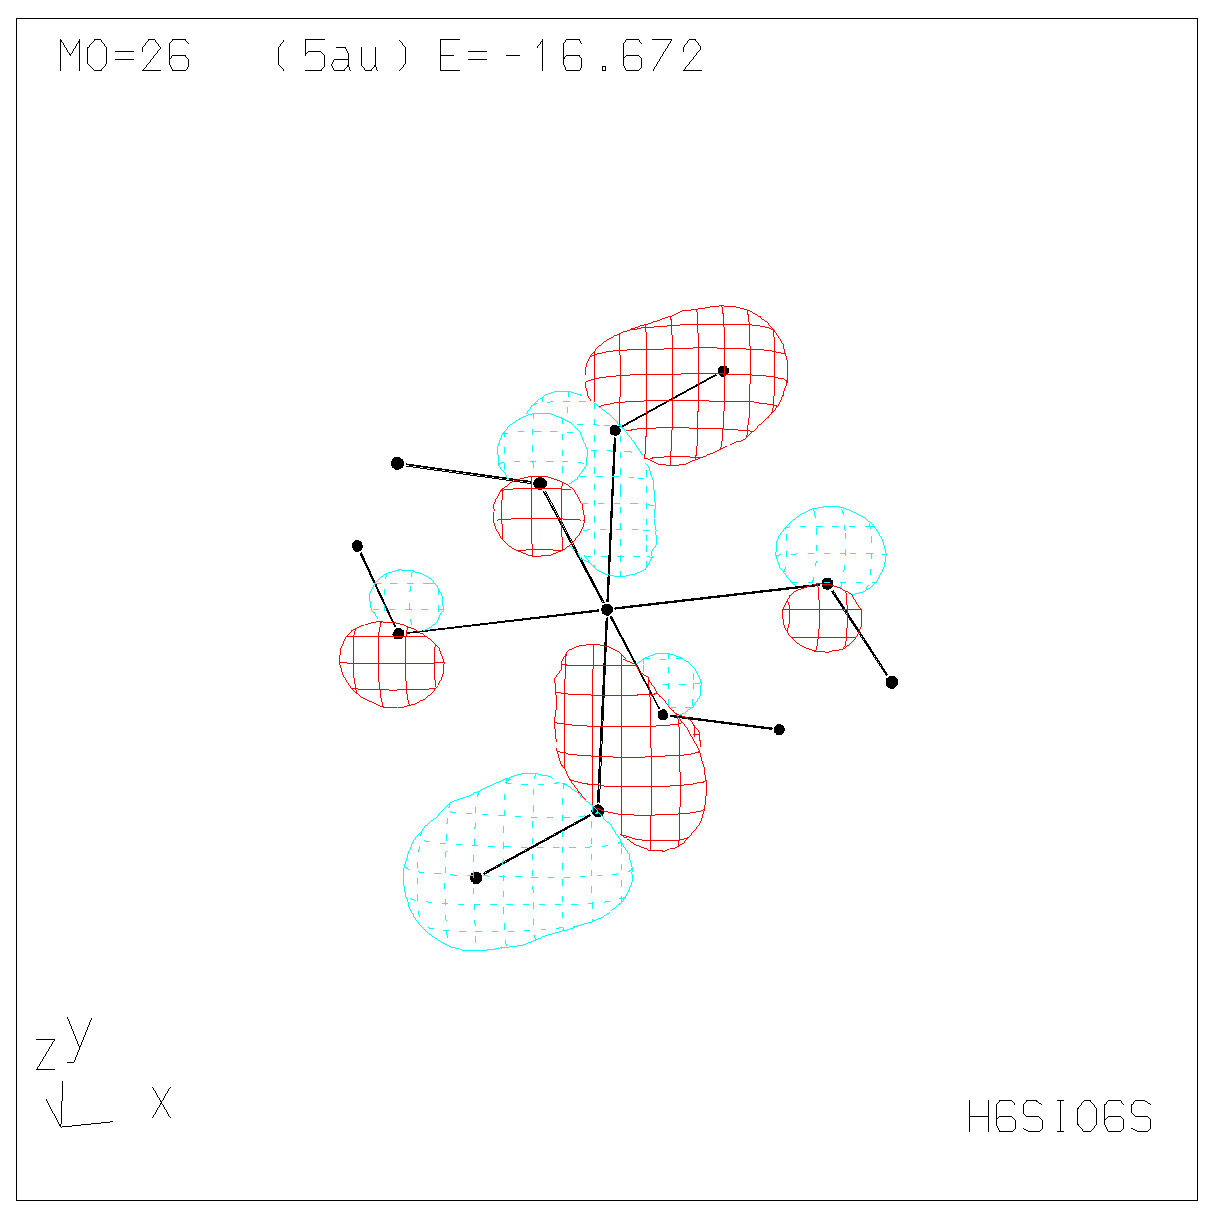
\includegraphics[width=5cm]{h6sio6_obrazky/s2_26.eps}\label{obr_h6sio6_MO_s2_26}}
\subfigure[MO 32]{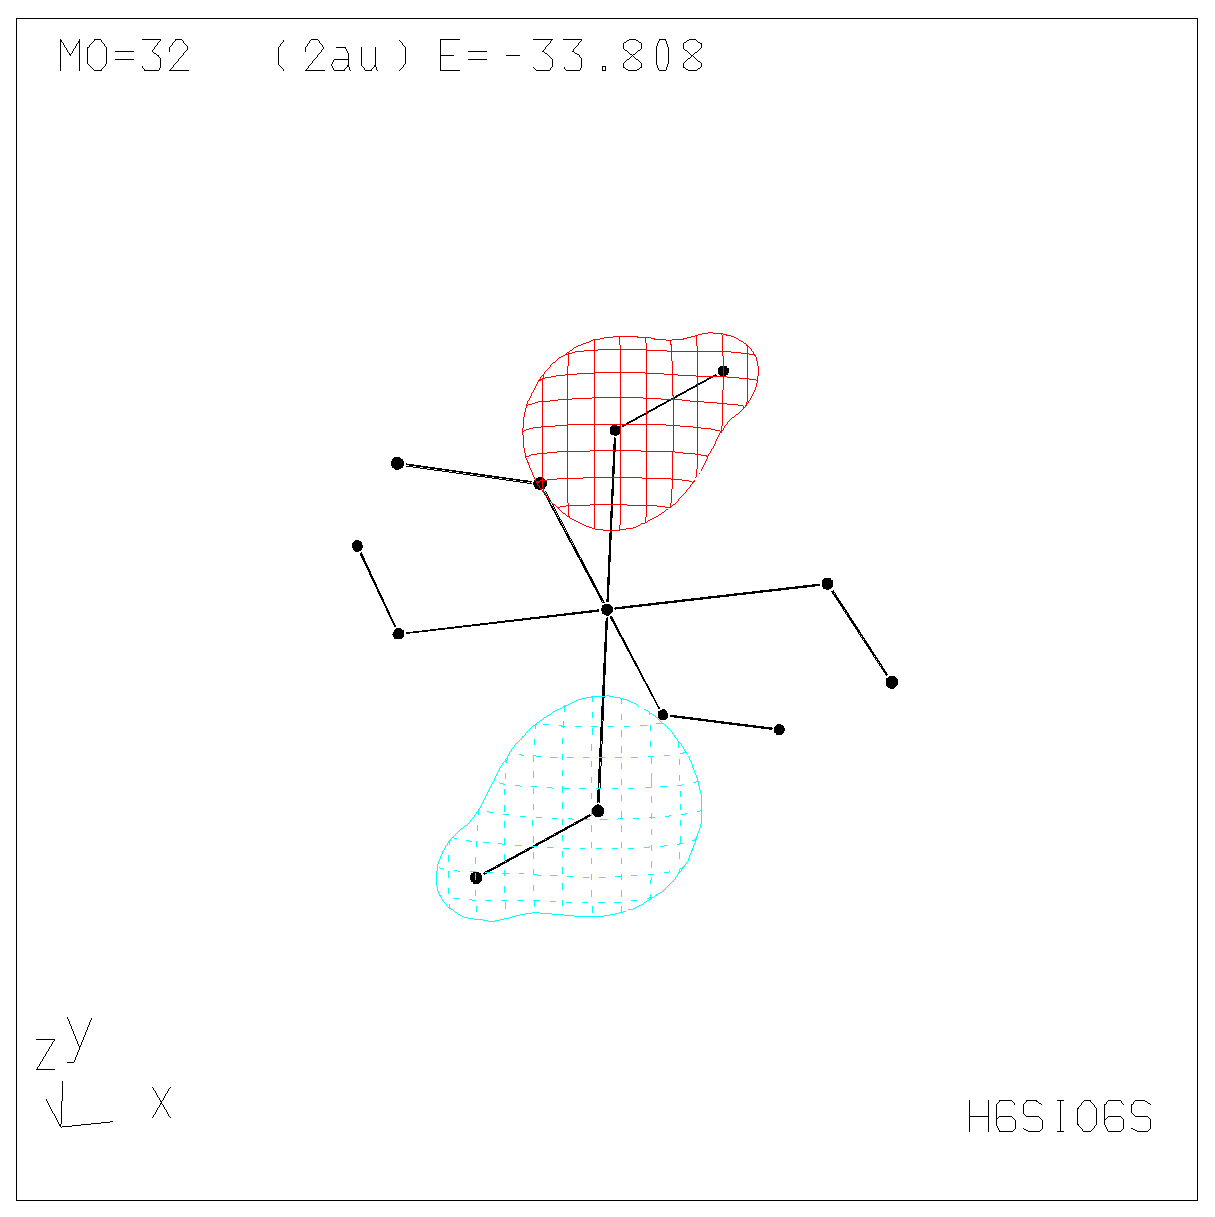
\includegraphics[width=5cm]{h6sio6_obrazky/s2_32.eps} \label{obr_h6sio6_MO_s2_32}}
\caption{Interakce $\bra{21}{\hat{H}}\ket{32}$, $\bra{28}{\hat{H}}\ket{32}$ z~tabulky \ref{tab_h6sio6_vysledky}.}

\label{obr_h6sio6_vysledky_II}\end{center}
\end{figure} 
 
    
\begin{figure}
\begin{center}
\subfigure[MO 2]{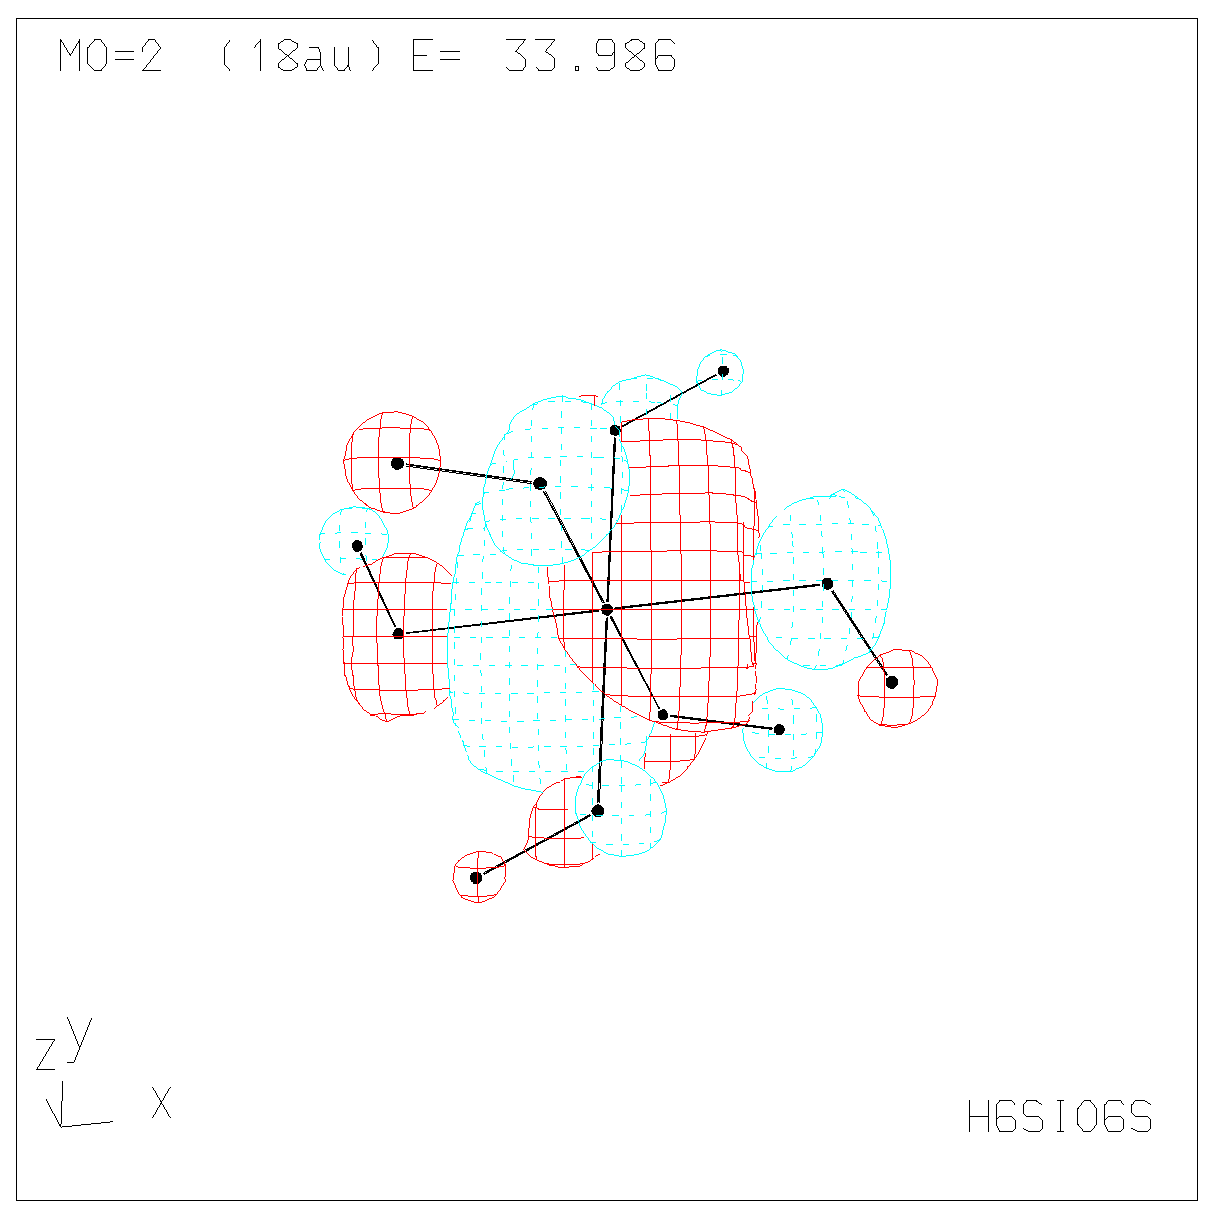
\includegraphics[width=5cm]{h6sio6_obrazky/s3_2.eps} 
\label{obr_h6sio6_MO_s3_2}}
\caption{Interakce $\bra{22}{\hat{H}}\ket{33}$ z~tabulky \ref{tab_h6sio6_vysledky}.}

\label{obr_h6sio6_vysledky_III}\end{center}
\end{figure} 
%----------------------------------------------------------------------------------------
 \subsection{Molekula H$_3$SiO$_4$(H$_2$PO$_3$)}
 Pro molekulu\ce{H3SiO4(H2PO3)} \ref{obr_h3sio4_h2po3} byla nutná oprava zvolených fragmentů. Molekula postrádá symetrii, která by usnadňovala výpočet. Jako fragment jedna byla zvolena část \ce{Si(OH)3} a~fragment dva byl \ce{O(H2PO3)}. Tato úprava usnadnila výpočetní náročnost a~bylo možné získat informace o~FMO. Fragmentové orbitaly  7, 15, 19, 22 a~29 se navzájem mísí za vzniku MO číslo 4, 14, 30, 35 a~41 znázorněných na obrázku \ref{obr_sio3p_vysledky_I}.   

\begin{figure}
\begin{center}
\subfigure[Interakční diagram pro \ce{H3SiO4(H2PO3)}.]{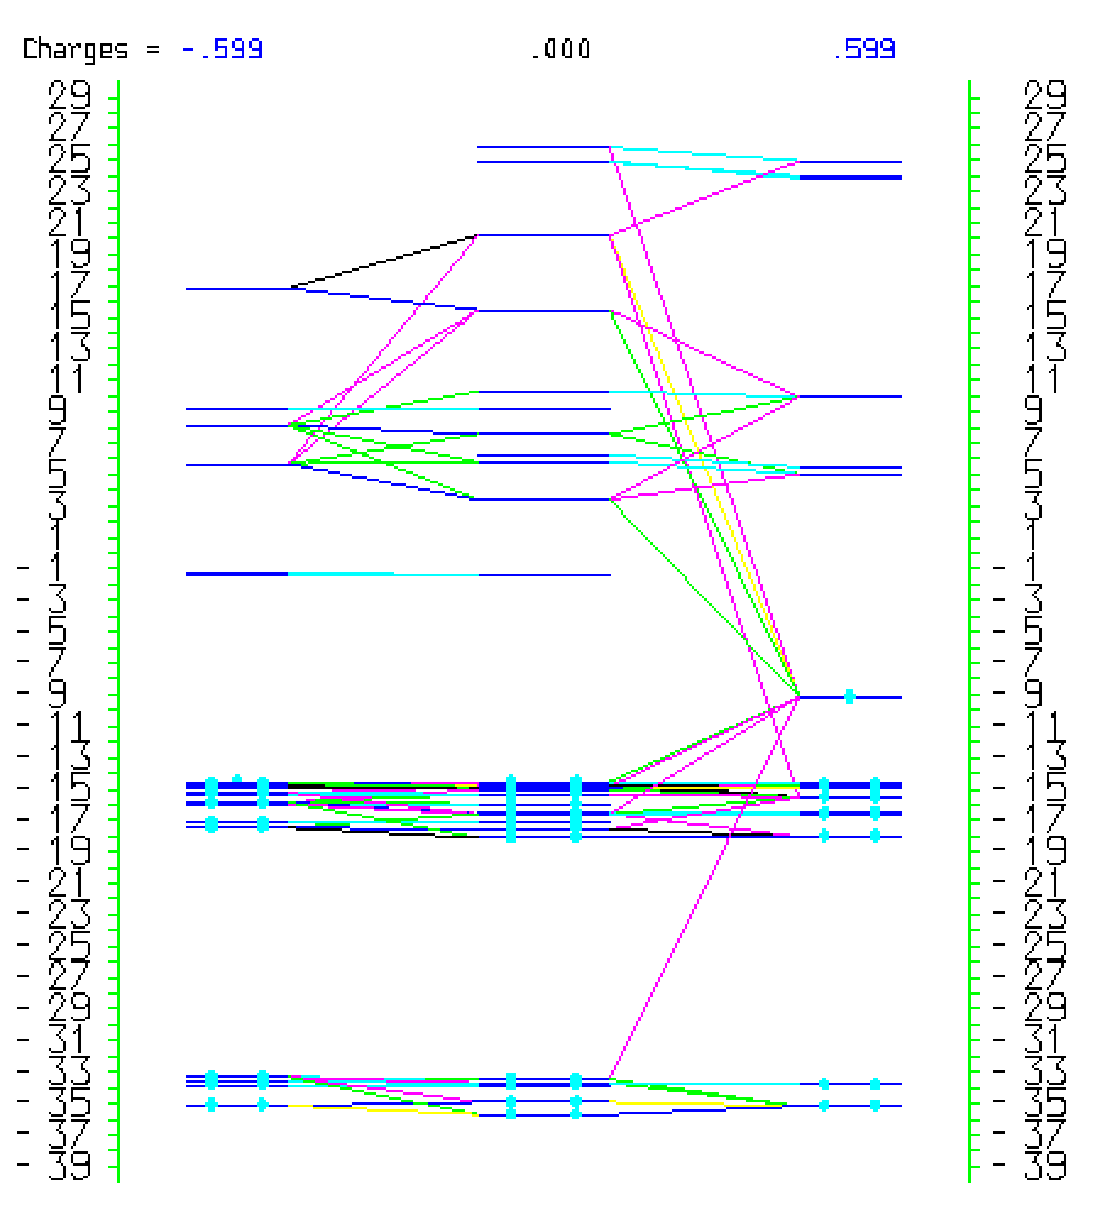
\includegraphics[width=5cm]{h3sio3P_diagram.eps} \label{h3sio4_h2po3_diagram_upraveny}}
\subfigure[Optimalizovaná struktura \ce{H3SiO4(H2PO3)}.]{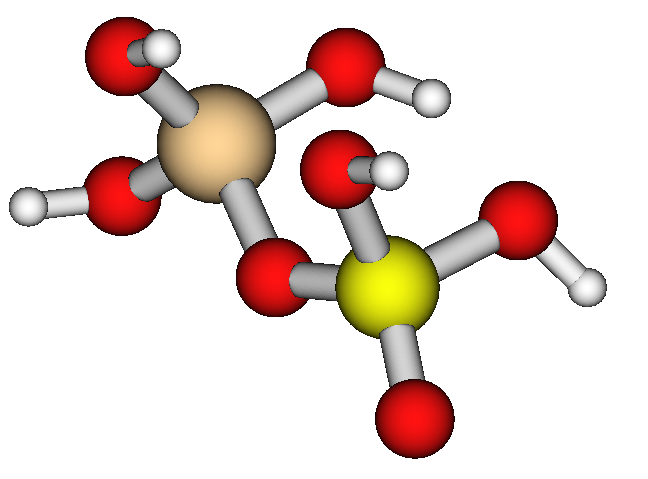
\includegraphics[width=5cm]{obr_h3sio4_h2po3.png}\label{obr_h3sio4_h2po3}}
\label{obr_SiOH3OH2PO)_vysledky_I}
\end{center}
\end{figure}

\begin{table}[htbp]
\caption{Výsledné mísení orbitalů pro \ce{H3SiO4(H2PO3)}}
\begin{center}
\begin{tabular}{|r|r|}
\hline
\multicolumn{2}{|c|}{$\bra{19}{\hat{H}}\ket{29}$, $\bra{15}{\hat{H}}\ket{29}$,$\bra{7}{\hat{H}}\ket{29}$, $\bra{22}{\hat{H}}\ket{29}$} \\
\hline \hline
\multicolumn{1}{|l|}{MO} & \multicolumn{1}{r|}{W} \\ \hline
4 & 32 \\ \hline
14 & 73 \\ \hline
30 & 63 \\ \hline
35 & 83 \\ \hline
41 & 46 \\ \hline
\end{tabular}

\label{tab_sio3_vysledky}\end{center}
\end{table}

 
\begin{figure}
\begin{center}
\subfigure[MO 4]{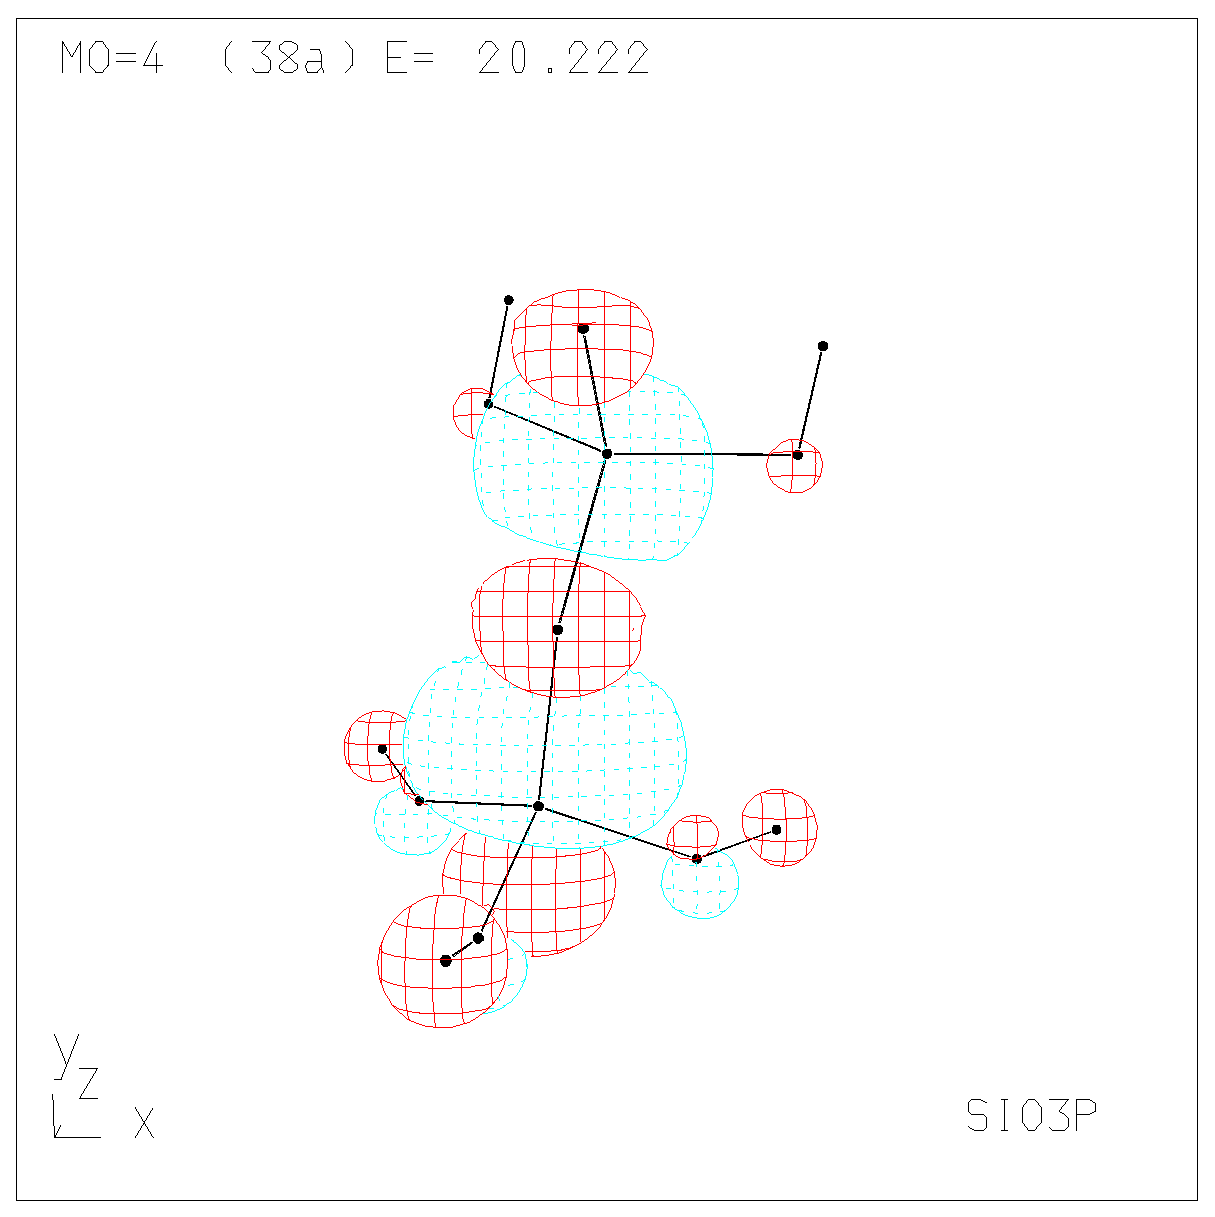
\includegraphics[width=5cm]{sio3p_obrazky/mo_4.eps} 
\label{obr_sio3_MO_4}}
\subfigure[MO 14]{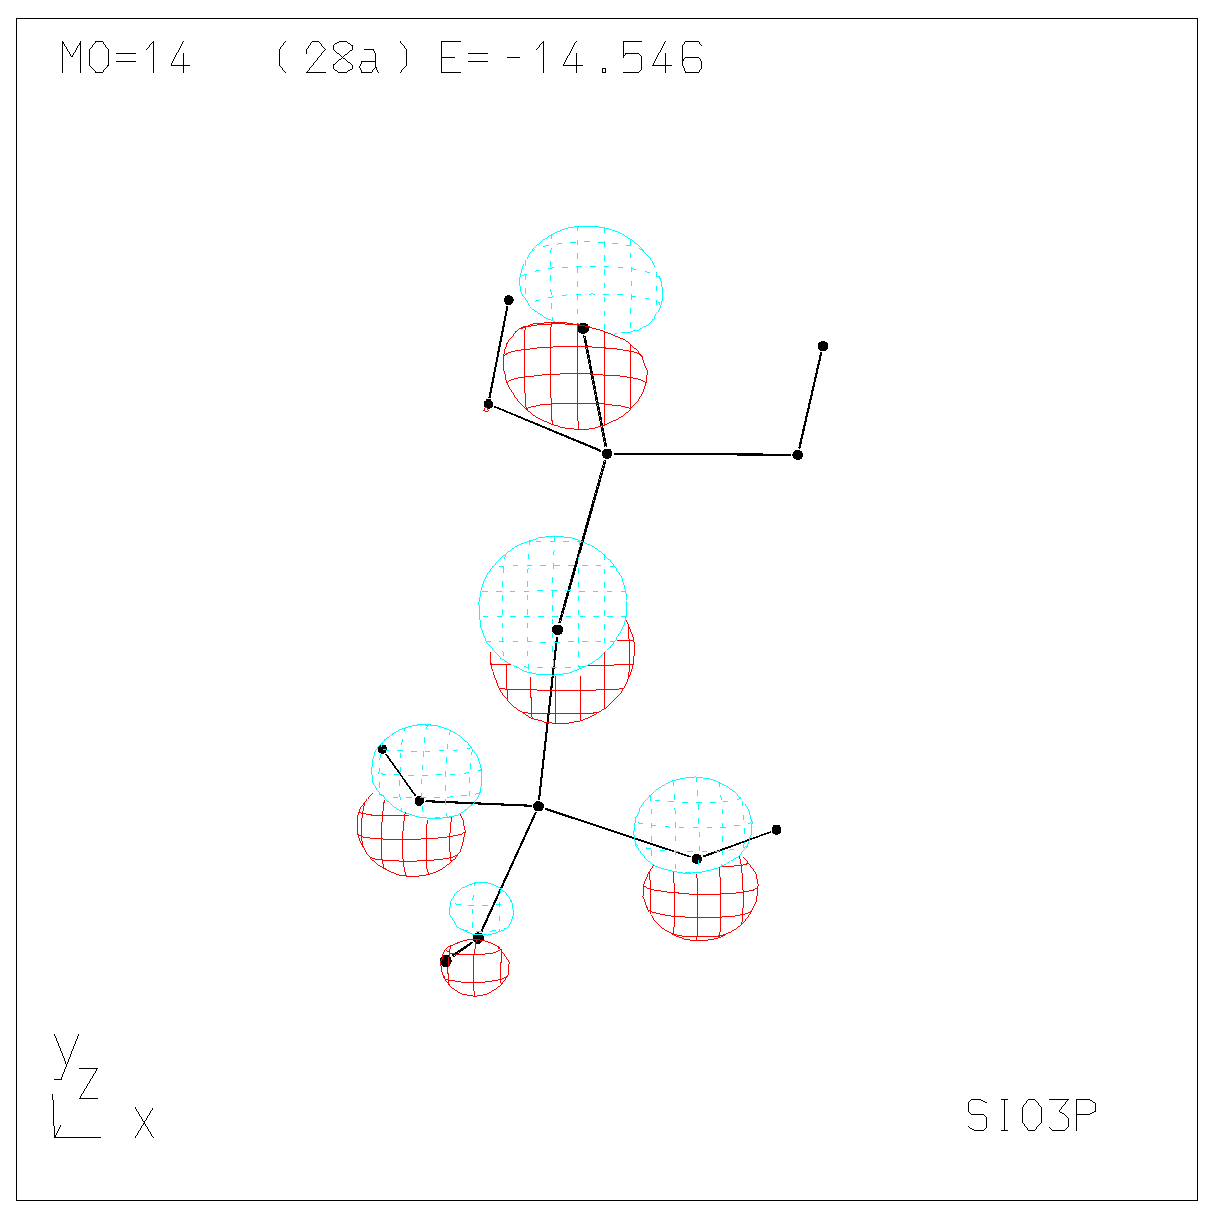
\includegraphics[width=5cm]{sio3p_obrazky/mo_14.eps} 
\label{obr_sio3_MO_14}}
\subfigure[MO 30]{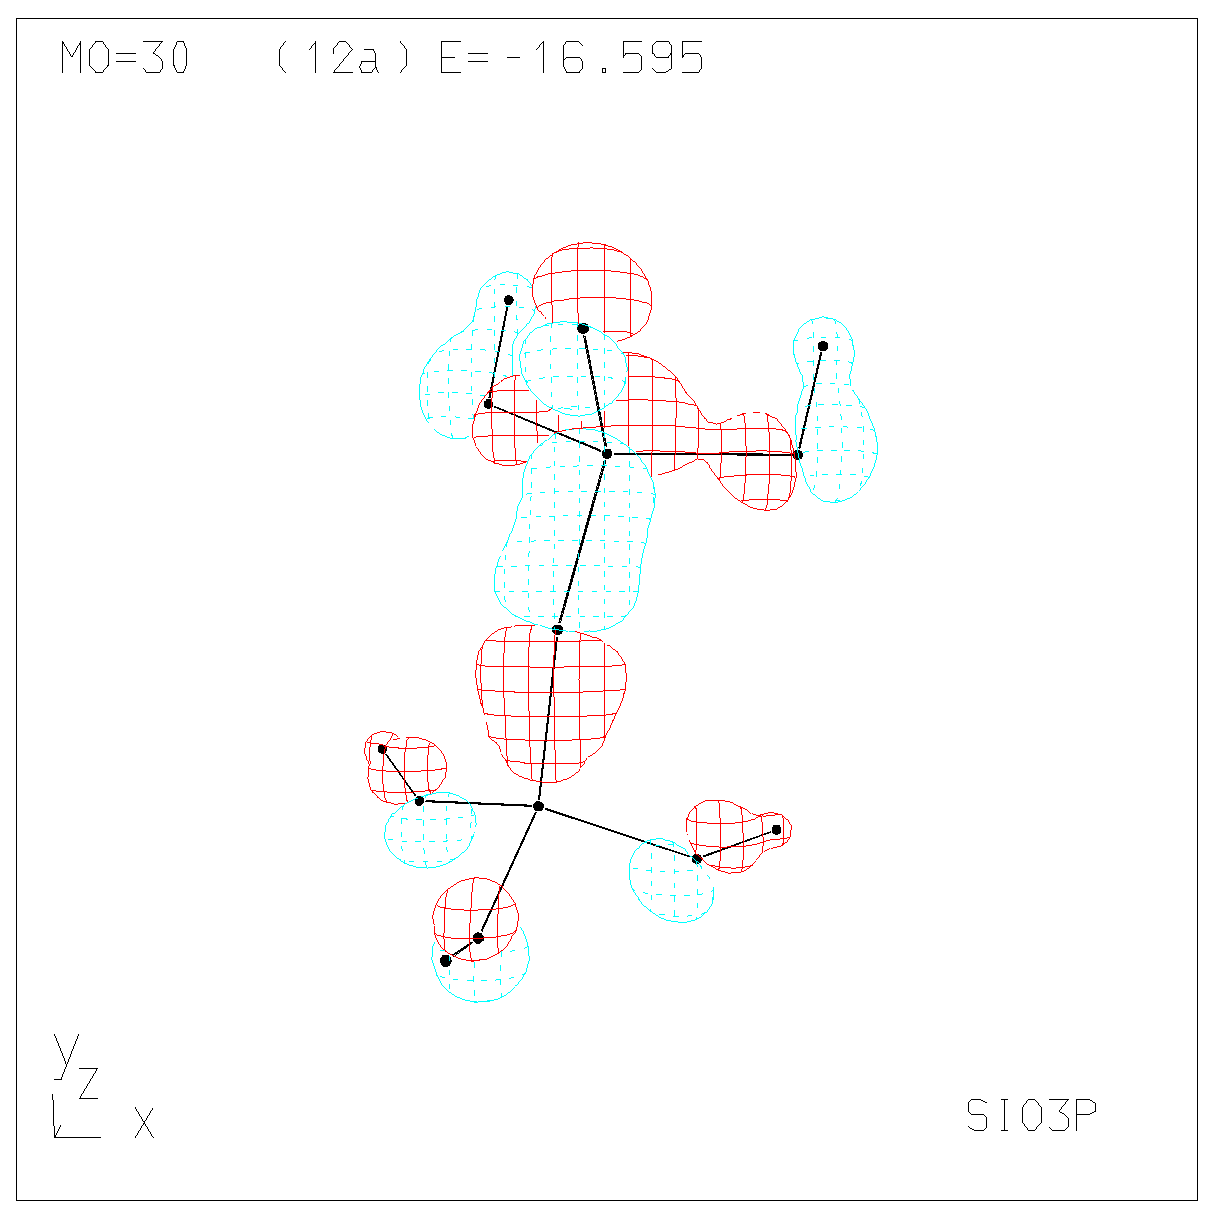
\includegraphics[width=5cm]{sio3p_obrazky/mo_30.eps} 
\label{obr_sio3_MO_30}}
\subfigure[MO 35]{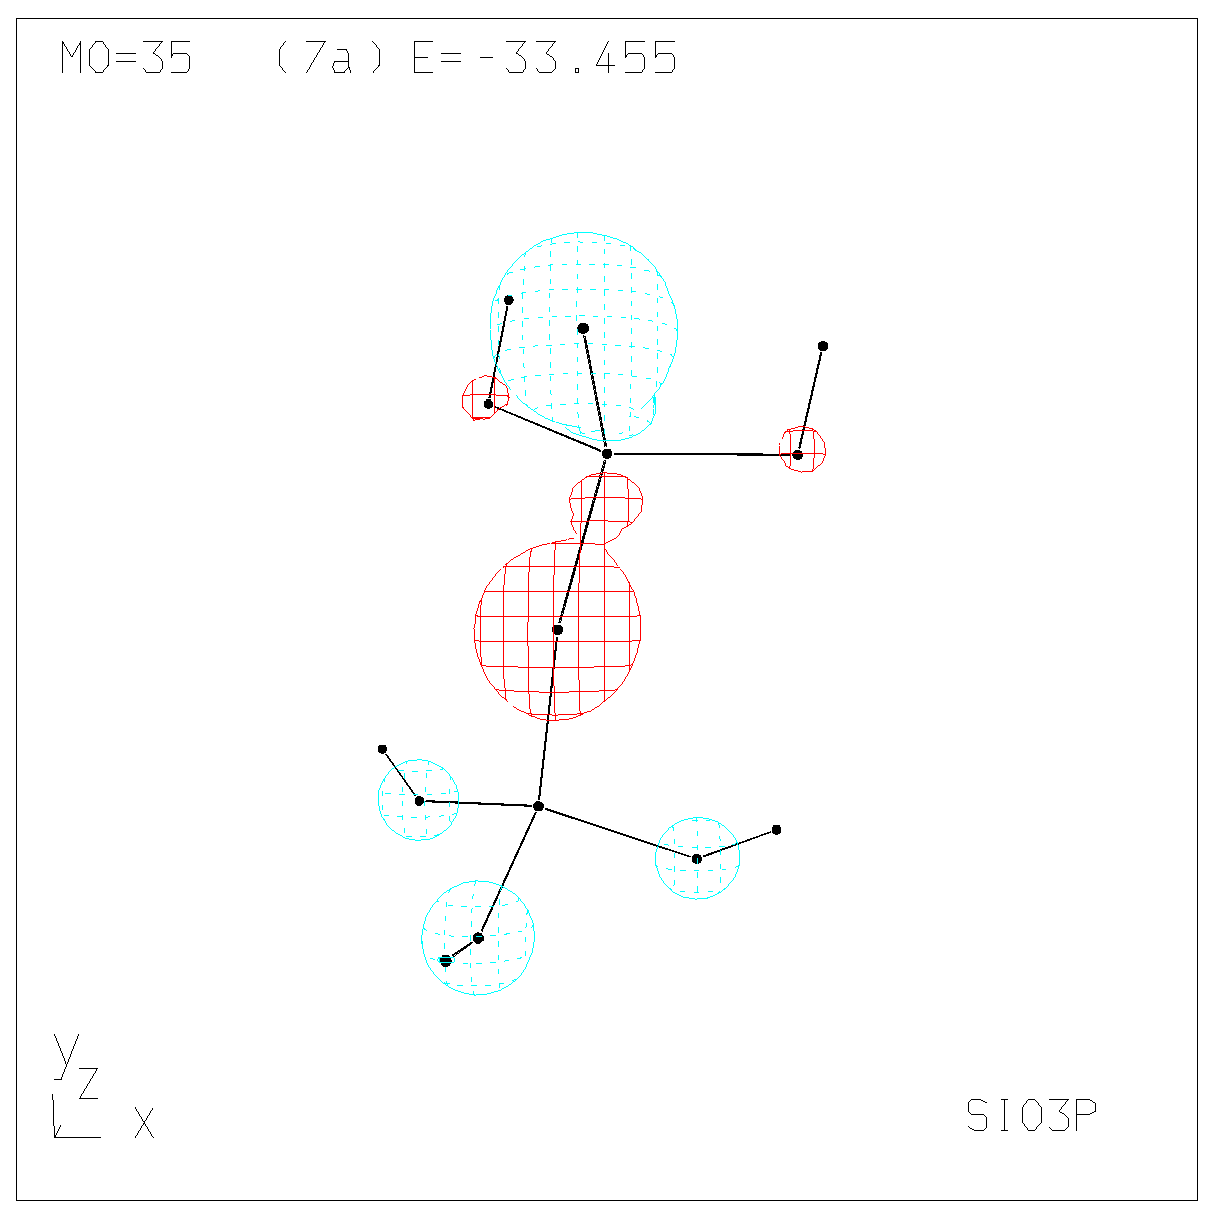
\includegraphics[width=5cm]{sio3p_obrazky/mo_35.eps} 
\label{obr_sio3_MO_35}}
\subfigure[MO 41]{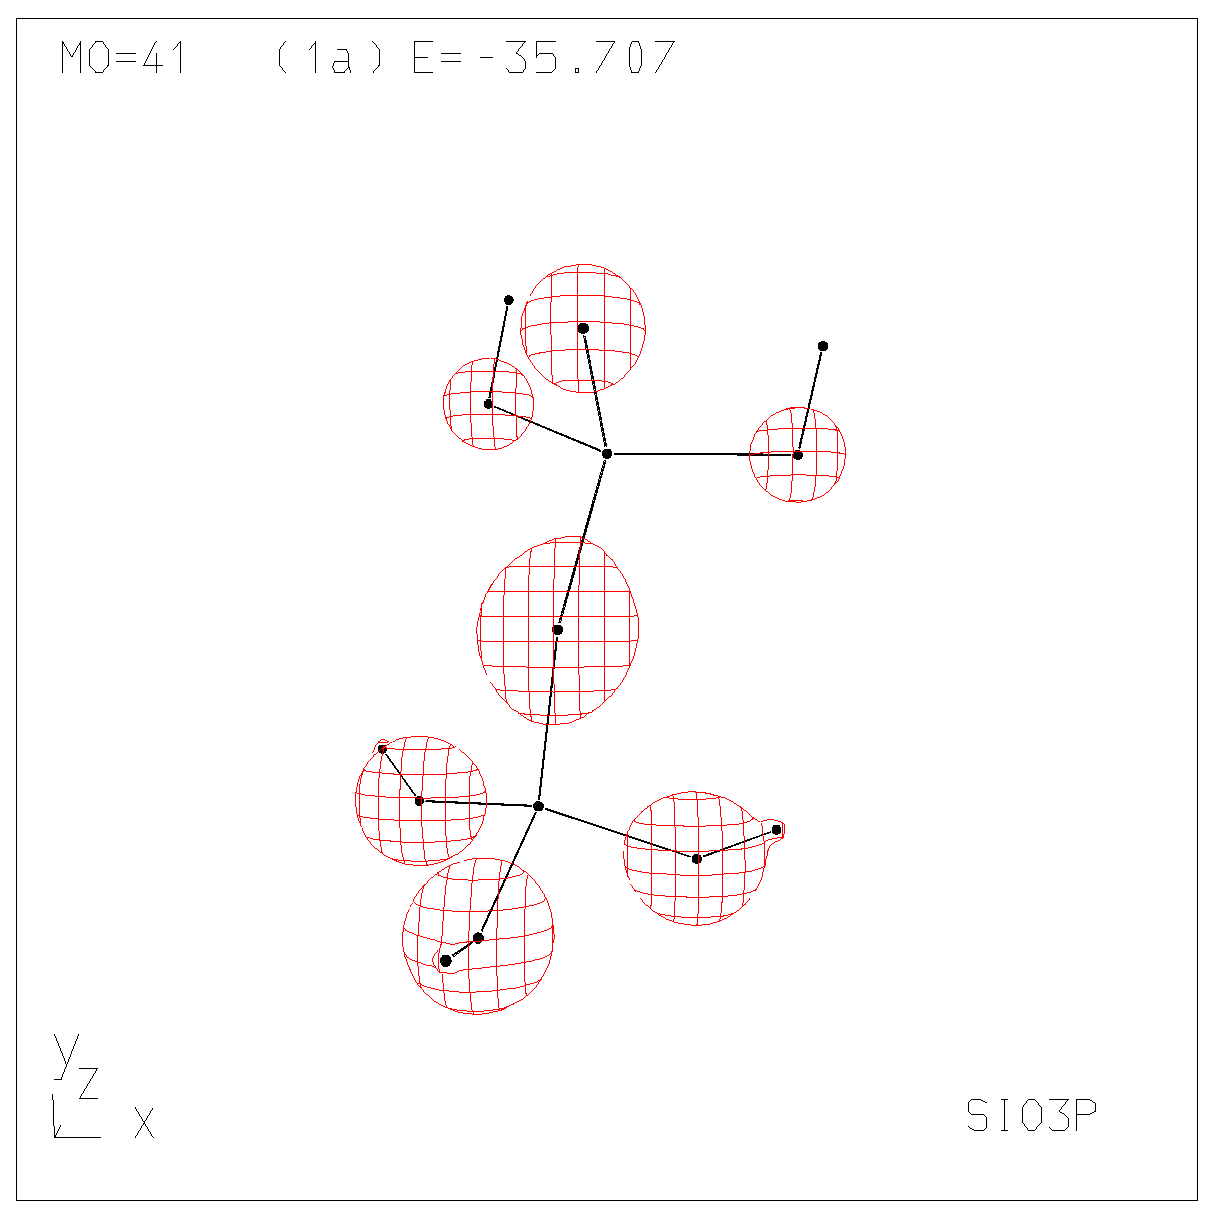
\includegraphics[width=5cm]{sio3p_obrazky/mo_41.eps} 
\label{obr_sio3_MO_41}}
\caption{Interakce $\bra{19}{\hat{H}}\ket{29}$, $\bra{15}{\hat{H}}\ket{29}$,$\bra{7}{\hat{H}}\ket{29}$, $\bra{22}{\hat{H}}\ket{29}$ z~tabulky \ref{tab_sio3_vysledky}.}

\label{obr_sio3p_vysledky_I}\end{center}
\end{figure} 
  
\section{DFT výpočet} \label{kapitola_DFT}
Pro DFT výpočty byly zvoleny molekuly, kde byl křemík koordinován čtyřmi i šesti kyslíky. Při konstrukci QM modelů molekul se zpočátku vyskytly potíže. Pro systém, kde byl křemík koordinován ve svém okolí šesti fosforečnany, docházelo k~umělému vytvoření vodíkových vazeb a~sytém se nepodařilo optimalizovat. Z~tohoto důvodu bylo nutné použít jako výchozí molekulu křemík koordinovaný šesti fosforečnany, které byly zároveň spojeny jednotkami \ce{SiO4}, viz. obrázek \ref{obr_si_o_poh3_6_propojeno_si}. Další komplikací při optimalizaci geometrické struktury byl celkový náboj molekuly, který byl nakonec určen jako $2-$, viz. výpočet níže. \\
Pro výpočet absolutního chemického stínění byla na křemík a~jeho bezprostřední okolí použita báze IGLO$-$III. Ostatní atomy byly počítány s~bazí 6-31G*. 
\begin{displaymath}
\ce{Si}^{4+} + \ce{(HPO4)^{2-}} + \ce{Si3^{4+}} + \ce{(OH)6^1-} = \ce{Si(HPO4)Si3(OH)6)^{2-}}
\end{displaymath}

\begin{figure}
\begin{center}
\subfigure[	\ce{H4SiO4}]{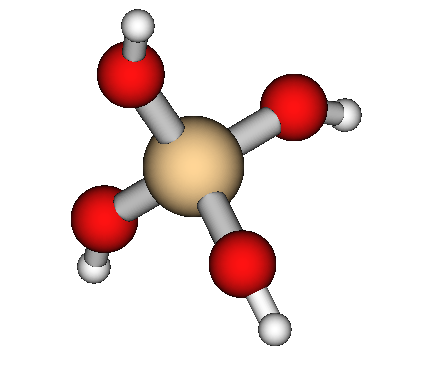
\includegraphics[width=5cm]{h4sio4_obr.png} 
\label{obr_h4sio4_II}}
\subfigure[\ce{(H6SiO6)^{2-}}]{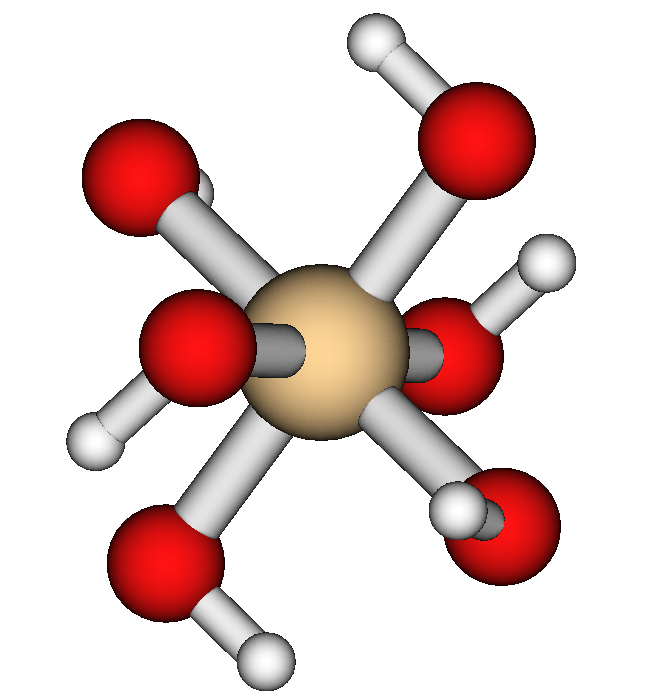
\includegraphics[width=5cm]{obr_h6sio6.png} 
\label{obr_h6sio6_II}}
\subfigure[ \ce{H3SiO3CH3}]{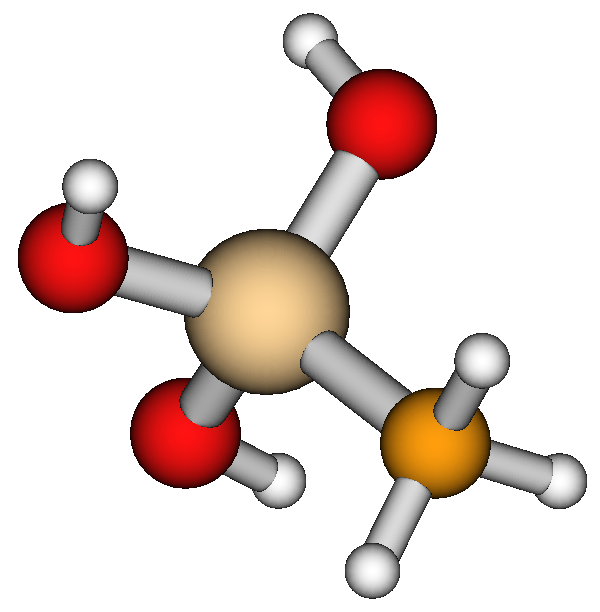
\includegraphics[width=5cm]{si(oh)3ch3_obr.png} 
\label{obr_h3sio3ch3}}
\subfigure[\ce{(H5SiO5CH3)^{2-}} ]{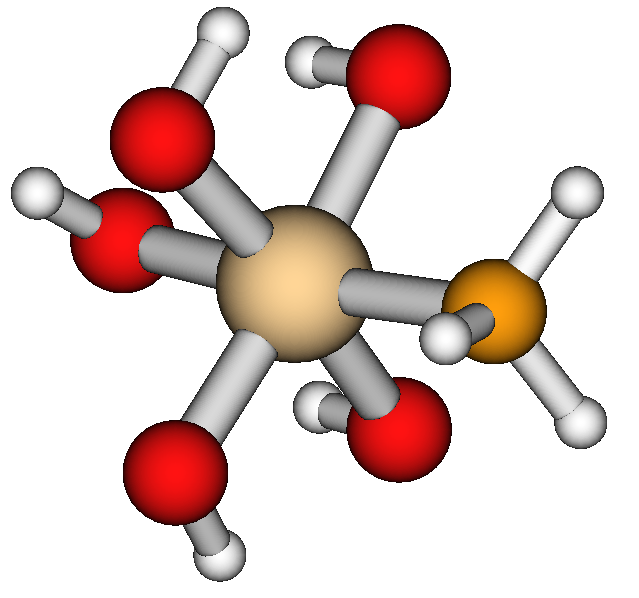
\includegraphics[width=5cm]{obr_h5sio5ch3.png} 
\label{obr_h5sio5ch3}}
\subfigure[\ce{H3SiO4(H2PO3)}]{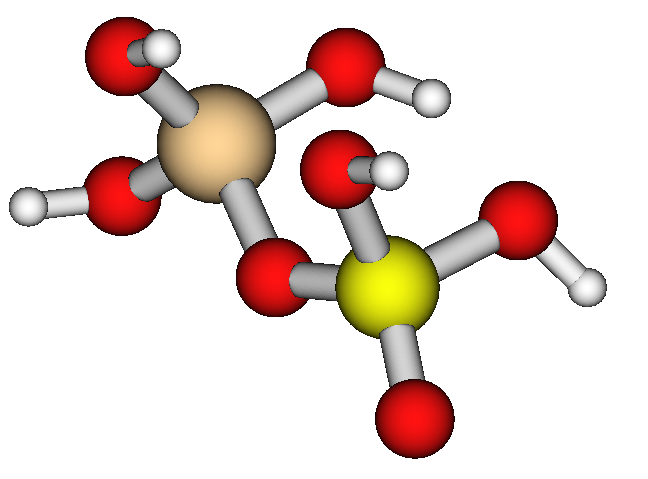
\includegraphics[width=5cm]{obr_h3sio4_h2po3.png} 
\label{obr_h3sio4_h2po3}}
\subfigure[\ce{SiO4(H2PO3)4}]{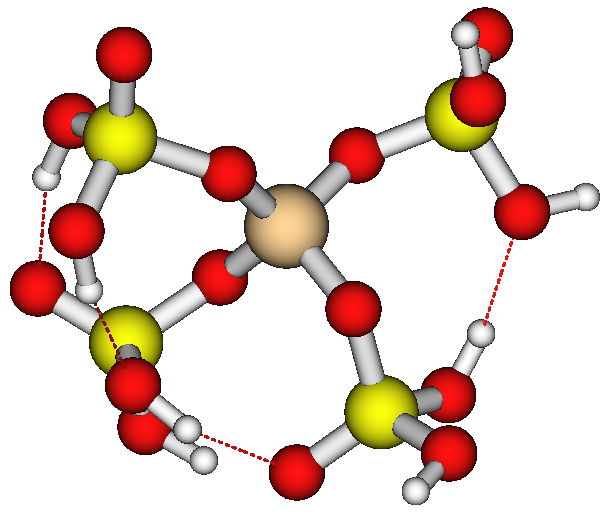
\includegraphics[width=5cm]{obr_sio4_h2po3_4.png} 
\label{obr_sio4_h2po3_4}}
\caption{Optimalizované struktury sloučenin křemíku}
\label{tab_vysledky_dft_I}\end{center}
\end{figure} 

\begin{figure}
\begin{center}
\subfigure[\ce{(SiO6(H2PO3)6(SiO4)6)^{2-}}]{\includegraphics[width=5cm]{obr_si_kryst_struktura.png} 
\label{obr_sobr_si_kryst_struktura}}
\subfigure[\ce{(Si^{VI}(PO4)6(Si^{IV}O4Et2)6)^{2-}} ]{\includegraphics[width=5cm]{obr_si_kryst_struktura_real.png} 
\label{obr_si_kryst_struktura_real}}
\subfigure[\ce{(Si(PO4)4(C2CH3)2(Si(OH)2)6)^{4-}}]{\includegraphics[width=5cm]{obr_si_o_poh_propojeno_si_jeden_kruh.png} 
\label{obr_si_o_poh3_6_propojeno_si}}
\caption{Optimalizované struktury křemičitofosfátů}
\end{center}
\end{figure}

\begin{table}[htbp]
\begin{minipage}{\textwidth}
\caption{Srovnání energiových parametrů pro vybrané struktury}
\begin{center}
\begin{tabular}{|l|r|r|r|r|}
\hline
 & E$_{\ce{H}}$\footnote{HOMO $-$ Highest Occupied Molecular Orbital} [eV] & E$_{\ce{L}}$\footnote{LUMO$ - $Lowest Unoccupied Molecular Orbital} [eV]& $\chi$ [eV] & $\eta$ [eV] \\ \hline
\hline
\ce{H4SiO4}  & -7,730 & 1,677 & 3,026 & 4,703 \\ \hline
\ce{(H6SiO6)^{2-}}  & 3,610 & 11,697 &  -7,653 & 4,043 \\ \hline
\ce{H3SiO3CH3}  & -7,750 & 0,825 &  3,462 & 4,287 \\ \hline
\ce{(H5SiO5CH3)^{2-}}  & 3,883 & 11,550 &  -7,716 & 3,834 \\ \hline
\ce{H3SiO4(H2PO3)} & -8,567 & 0,060 &  4,254 & 4,314 \\ \hline
\ce{SiO4(H2PO3)4} & -8,088 & -0,829 & 4,459 & 3,629 \\ \hline
\ce{(SiO6(H2PO3)6)^{2-}} & - \footnote{Strukturu se nepodařilo optimalizovat z~důvodu nestability}& - & -& - \\ \hline
\ce{Si(H2PO3)3OH} & - \footnote{Strukturu se nepodařilo optimalizovat z~důvodu tvorby umělých vodíkových můstků} & - & - & - \\ \hline
\ce{(Si(H2PO3)5OH)^{2-}} & - \footnote{Strukturu se nepodařilo optimalizovat z~důvodu nestability} & - & - & - \\ \hline
\ce{(Si(PO4)6(Si(OH)2)6)^{2-}} \footnote{Optimalizace s~bazí IGLO-III} & -3,670 & 4,040 &  -0,185 & 3,855 \\ \hline
\ce{(Si(PO4)6(Si(OH)2)6)^{2-}} \footnote{Optimalizace s~bazí 6-31G*}& -3,346 & 4,574 &  -0,614 & 3,960 \\ \hline
\ce{(Si^{VI}(PO4)6(Si^{IV}O4Et2)6)^{2-}} \footnote{VI a~IV jsou hodnoty koordinace křemíku, zdroj \cite{C3NJ00721A}} & -2,609 & 5,109 & -1,250 & 3,859 \\ \hline
\ce{(Si(PO4)4(C2CH3)2(Si(OH)2)6)^{4-}} \footnote{Fosfor je nahrazen uhlíkem v~rámci jednoho kruhu}& 5,366 & 10,467 &  -7,916 & 2,550 \\ \hline
\end{tabular}
\end{center}
\label{tab_porovnani_molekul_dft}
\end{minipage}
\end{table}

Z~tabulky \ref{tab_porovnani_molekul_dft} vyplývá, že struktury se čtyř koordinovaným křemíkem jsou stabilnější než struktury s~křemíkem v~koordinaci šest. Jedno z~kritérií stability výsledných molekul jsou hodnoty energie HOMO a~LUMO orbitalů. Především hypotetické molekuly \ce{(H5SiO5CH3)^{2-}} a~\ce{Si(PO4)4(C2CH3)2(Si(OH)2)6} (oba případy) vykazují kladnou hodnotu energie HOMO orbitalů. Výsledný parametr $\eta$ také poukazuje na stabilitu molekuly a~to podle teorie HSAB. Pro molekuly s~velkou hodnotou $\eta$ platí, že vykazují větší stabilitu. Hypotetické sloučeniny  \ce{(SiO6(H2PO3)6)^{2-}}, \ce{Si(H2PO3)3OH} a~\ce{(Si(H2PO3)5OH)^{2-}} se z~důvodu nestability nepodařilo vůbec optimalizovat. \\
Pro potřeby výpočtu NMR parametrů byla krystalická struktura upravena a~krajní ethyly byly nahrazeny vodíky. Absolutní chemické stínění bylo počítáno pro centrální šestikoordinovanný křemík. Hodnoty pro upravenou krystalovou strukturu měly k~dobrou shodu s~experimentálními hodnotami, které byly převzaty z~článku \cite{C3NJ00721A}. Z~toho lze usoudit, že úprava struktury neměla výraznější dopad na absolutní chemické stínění. 

\begin{table}[htbp]
\begin{minipage}{\textwidth}
\caption{Výsledky pro absolutní magnetické stínění upravené krystalové struktury \ref{obr_sobr_si_kryst_struktura}.}
\begin{center}
\begin{tabular}{|r|r|r|}
\hline
\multicolumn{1}{|l|}{Ćíslo atomu} & \multicolumn{1}{l|}{Abs. magn. stínění [ppm]} & \multicolumn{1}{l|}{Chem. posuv \footnote{Experimentální hodnoty \cite{1316862}} [ppm]} \\ \hline
1 & 546,5 & -101 \\ \hline
43 & 433,0 & -212 \\ \hline
44 & 432,9 & -212 \\ \hline
45 & 432,1 & -212 \\ \hline
46 & 432,9 & -212 \\ \hline
47 & 432,9 & -212 \\ \hline
48 & 432,3 & -212 \\ \hline
\end{tabular}
\end{center}
\label{vysledky_abs_magn_stineni}
\end{minipage}
\end{table}

  
  \chapter{Závěr}
Cílem této bakalářské práce bylo určit tvrdost/měkkost vybraných křemičitofosfátů a~různých modifikací. Z~těchto parametrů lze dále usuzovat stabilitu vzniklých sloučenin a~jejich ochotu reagovat s~dalšími látkami. Další s~problémů bylo vysvětlit neochotu křemíku přejít ze čtyřkoordinace na šestikoordinaci pokud měl na sebe přímo navázaný uhlík. Funkce uhlíku jako destabilizujícího prvku v~šestikoordinovanných sloučeninách křemíku byl možné pozorovat u~sloučeniny \ce{(H5SiO5CH3)^{2-}}, kde je energie HOMO i LUMO orbitalu kladná. Tento efekt bylo možné také pozorovat u~složitějších struktur, kde byl fosfor nahrazen za uhlík. Pokud byly nahrazeny fosfory na více než jednom kruhu, docházelo k~rozpadu sloučeniny. Zásadním problémem při optimalizaci molekul byla tvorba umělých vodíkových můstků. Z~tohoto důvodu bylo nutné rozšířit molekulu, aby se situace více přiblížila reálnému polymeru. \\
Krystalová struktura byla pro výpočet absolutního chemického stínění upravena, přesto byla dobrá shoda s~experimentem. Do budoucna by bylo zajímavé rozebrat i další modifikace křemičitofosfátů a~porovnat stabilitu vůči množství uhlíků vázaných na centrální křemík. 
  
  \chapter{Výpočetní detaily}
  Molekuly z~kapitoly \ref{kapitola_EHT} byly optimalizovány programem Gaussian \cite{g09}. Všechny optimalizace probíhaly s~hybridním funkcionálem B3LYP a~bazí 6-31G*. Struktury byly nejprve navrženy programem Avogadro \cite{Avogadro}, zobrazení výstupu z~Gaussianu bylo prováděno programem MOLDEN \cite{Molden}. Programem MOLDEN byly i tvořeny obrázky struktur. Optimalizovaná struktura byla použita jako vstup pro program C.A.C.A.O. \cite{cacao}. Z~interakčního diagramu a~analýzou FMO byly vybrány MO, které byly zobrázovány grafickým prostředím C.A.C.A.O. Stejným program byl i použit pro tvorbu interakčních diagramů. \\
  Molekuly z~kapitoly \ref{kapitola_DFT} byly také optimalizovány programem Gaussian, zároveň byl použit stejný funkcionál i báze. Použití stejné báze umožnilo vzájemné porovnání molekul. Pro výpočet NMR parametrů byla struktura optimalizována s~bazí IGLO-III, která byla implementována z~webové stránky  . Na centrální molekulu křemíku a~nejbližší okolí byla použitá báze IGLO$-$III, na vzdálené okolí báze 6-31G*. Báze IGLO$-$III pro atom křemíku a~kyslíku byla stažena z~webové stránky EMSL \cite{EMSL}. Vstupní soubory pro optimalizaci programem Gaussian jsou uvedeny jako příloha A. Při optimalizaci rentgenové struktury byla molekula nejprve zobrazena programem Mercury \cite{Mercury}, následně byl proveden výpočet optimalizace programem Gaussian.
  
{\csname captions\languagename\endcsname %% Temporarily override
%% the BibLaTeX localization with the original babel definitions.
\makeatletter %% Use the correct localization of the quotations.
  \thesis@selectLocale{\thesis@locale}\makeatother
\printbibliography[heading=bibintoc]} %% Print the bibliography.
\appendix %% Start the appendices.
\chapter{Přílohy}
 \begin{lstlisting}[frame=single, caption={\ce{H4SiO4} },label=DescriptiveLabel]
OPT H4SIO4 

0 1
SI  1   .000   .000   .000 
O  2   .000 -1.349   .954 
H  3  -.750 -1.453  1.557 
O  4  1.349   .000  -.954 
O  5   .000  1.349   .954 
O  6 -1.349   .000  -.954 
H  7  1.453  -.750 -1.557 
H  8   .750  1.453  1.557 
H  9 -1.453   .750 -1.557 
 \end{lstlisting}

 \begin{lstlisting}[frame=single, caption={\ce{(H6SiO6)^{2-}} },label=DescriptiveLabel]
OPT H6SIO6 

-2 1
SI   .000   .000   .000  
O   .000   .000 -1.652 
O  1.652   .000   .000 
O   .000 -1.652   .000 
H   .866   .000 -2.085 
H  2.085  -.866   .000 
H  -.866 -2.085   .000 
O   .000   .000  1.652 
O -1.652   .000   .000 
O   .000  1.652   .000 
H  -.866   .000  2.085 
H -2.085   .866   .000 
H   .866  2.085   .000
 \end{lstlisting}
  
  \newpage
  
  \begin{lstlisting}[frame=single, caption={\ce{H3SiO3CH3}},label=DescriptiveLabel]
OPT H3SIO3CH3

0 1
Si        -0.93401        0.43592       -0.98471
O         -2.03997       -0.48875       -0.31004
H         -2.23645       -0.99494        0.35857
O         -0.55798       -0.13126       -2.42355
H          0.06732       -0.44366       -2.92683
O         -1.47925        1.92557       -1.11519
H         -1.36662        2.74938       -0.89044
C          0.59507        0.43830        0.08739
H          1.37120        1.08100       -0.37659
H          0.98140       -0.59723        0.18307
H          0.34130        0.83253        1.09283
 \end{lstlisting}

\begin{lstlisting}[frame=single, caption={\ce{H5SiO5CH3}},label=DescriptiveLabel]
OPT H5SIO5CH3

-2 1
Si        -0.05446       -0.05417        0.00151
O         -1.25911        0.47123       -0.90554
H         -2.04028        0.83732       -0.91639
O         -0.02244       -1.41252       -0.83536
H          0.07095       -1.76839       -1.61560
O          1.13825       -0.59195        0.91385
H          1.68837       -1.23964        1.06136
O          0.99948        0.58879       -1.00877
H          1.76367        0.97919       -1.09334
O         -1.10698       -0.70022        1.01320
H         -1.63759       -1.36222        1.16938
C         -0.08214        1.58320        0.98745
H          0.94880        1.97923        1.11669
H         -0.53656        1.48968        1.99698
H         -0.64366        2.36871        0.43820

 \end{lstlisting}
 \newpage
 

\begin{lstlisting}[frame=single, caption={\ce{H3SiO4(H2PO3)}},label=DescriptiveLabel]
OPT H3SIO4POH3

0 1
Si        -0.17389       -0.68992        0.09187
O         -1.37171       -1.10768       -0.86938
H         -1.90255       -0.85573       -1.49914
O          1.20675       -1.23623       -0.48131
H          1.93595       -1.03849       -0.89488
O         -0.42347       -1.28722        1.54568
H         -0.53750       -2.00055        2.01473
O         -0.11080        0.90003        0.19547
P          0.00865        2.29054       -0.61619
O          1.50200        2.21678        0.32214
H          1.33718        2.18898        1.30929
O          0.23992        3.81736        0.19126
H          0.38224        4.47244       -0.53982
O         -1.24444        2.52446        0.27085
 \end{lstlisting}

\newpage

\begin{lstlisting}[frame=single, caption={\ce{SiO4(H2PO3)4}},label=DescriptiveLabel]
OPT SIO4(H2PO3)4

0 1
Si        -1.67886        0.10962       -0.26584
O         -2.65396        0.16657        0.98886
O         -2.49892       -0.30809       -1.56252
O         -1.02190        1.54148       -0.48605
O         -0.53114       -0.96044       -0.00433
P         -3.90417        0.91776        1.66428
P          0.12835        2.56347       -0.02258
P          0.92630       -1.48158       -0.43802
P         -3.31301       -1.48394       -2.29603
O         -4.15324        0.16004        2.99498
O         -3.49406        2.55892        2.05354
H         -3.16086        2.94204        1.20323
O         -5.32427        0.74723        0.68078
H         -5.04023        1.03972       -0.22179
O          0.32107        2.46382        1.69996
H          0.88425        3.24347        1.93571
O         -0.41154        3.97176       -0.38913
O          1.58041        2.24921       -0.92033
H          2.18857        2.99375       -0.68285
O          0.96872       -2.96902        0.00224
O          2.15546       -0.60812        0.42208
H          2.99211       -1.10545        0.23963
O          1.08523       -1.41941       -2.16559
H          0.84652       -0.48877       -2.40596
O         -4.71745       -1.92229       -1.37491
H         -4.37466       -2.09201       -0.46137
O         -3.79620       -0.86104       -3.63223
O         -2.26132       -2.81159       -2.67589
H         -1.84439       -3.05574       -1.81140
 \end{lstlisting}
\newpage

\begin{lstlisting}[frame=single, caption={\ce{(Si(PO4)6(Si(OH)2)6)^{2-}}},label=DescriptiveLabel]
OPT SI(PO4)6(SI(OH)2)6

Si        -0.00115       -0.00493       -0.00808
O         -1.21958        0.47299       -0.92302
O         -1.01116       -0.91265        0.86961
O          0.26302       -1.25494       -1.02026
O          1.21643       -0.47100        0.91588
O          0.97838        0.90360       -0.90610
O         -0.24953        1.24968        0.97901
P         -2.72789        0.13058       -1.32125
P         -1.57504       -2.37867        1.24202
P          1.30298       -2.42873       -1.51870
P          2.73301       -0.21272        1.35960
P          1.31150        2.45005       -1.27906
P         -1.20317        2.41853        1.54715
O         -2.82079       -1.36681       -1.73612
O         -2.44803       -3.04601        0.06692
O         -0.28620       -3.23520        1.45424
O          1.41825       -3.61219       -0.39646
O          2.79210       -1.82122       -1.81247
O          3.62599       -0.42570        0.09398
O          2.95917        1.31616        1.74624
O          2.10210        3.06658       -0.00503
O         -0.06497        3.29051       -1.59220
O         -1.50400        3.54482        0.46303
O         -2.59586        1.75296        1.86645
O         -3.53849        0.20564        0.03328
O         -3.33630        1.01013       -2.44787
O         -2.35170       -2.42169        2.58524
O          0.74392       -3.09075       -2.81279
O          3.25956       -1.17775        2.45561
O          2.28622        2.50508       -2.48777
O         -0.65635        3.11763        2.81971
O         -4.88397       -2.40960       -0.78227
O         -3.18509       -3.67192       -2.39855
O          1.50278       -4.63267        2.14123
O          4.86303       -2.57482       -0.28865
O          5.22630       -0.46316       -1.65215
O          4.67467        2.79903        0.49652
O          3.03933        3.77526        2.34560
O         -0.16802        5.54640       -0.47511
O         -2.50784        4.66839       -1.59017
O         -4.37440        2.35265        0.12711
O         -4.61760        0.33547        2.25381
Si        -3.36546       -2.69620       -1.18091
Si         0.67201       -4.28798        0.87415
Si         4.12070       -1.37639       -1.00562
Si         3.20056        2.76015        1.13039
Si        -1.08928        4.28823       -0.85266
Si        -3.87351        1.21446        1.14136
H         -5.50540       -1.81345       -0.86170
O         -0.14416       -5.61947        0.66363
H         -4.41141       -0.31621        2.79833
H         -0.48313       -6.22474        1.18093
H          1.28172       -4.88954        2.93467
H          5.36821        3.21822        0.19716
H          5.85399        0.04601       -1.34067
H          5.33908       -2.73802        0.41084
H         -4.19920        2.56846       -0.70505
H         -3.38124        4.59596       -1.64921
H          0.66077        5.80806       -0.47523
H          2.57317        3.93579        3.05453
H         -2.82697       -3.66462       -3.18196
 \end{lstlisting}
 \begin{lstlisting}[frame=single, caption={\ce{Si^{VI}(PO4)6(Si^{IV}O4Et2)6}},label=DescriptiveLabel]
OPT KRYST.STRUKTURA

-2  1
Si       7.32701         3.07856         6.25613
O        6.92240         3.12292         7.79313
O        7.88487         1.59838         6.43045
O        5.86168         2.52021         5.88888
O        7.75659         3.03240         4.71001
O        6.78654         4.56061         6.06495
O        8.77527         3.64859         6.62635
P        6.50059         2.24960         9.06746
P        7.73171         0.07817         5.98978
P        4.70285         2.38223         4.76685
P        8.14133         3.92096         3.42439
P        6.98147         6.09090         6.50144
P        9.92153         3.78170         7.75271
O        5.58458         1.06543         8.56645
O        6.58508        -0.58976         6.89123
O        7.24043         0.10512         4.48574
O        5.03045         1.12369         3.82871
O        4.62429         3.70657         3.86913
O        6.82102         4.59396         2.82714
O        9.10922         5.09432         3.89393
O        8.17128         6.72198         5.65985
O        7.39608         6.15711         8.03734
O        9.55707         4.95262         8.77589
O        0.00305         2.44077         8.60624
O        7.80945         1.61162         9.73938
O        5.68665         3.08307        10.08295
O        9.06158        -0.71065         6.09472
O        3.31995         2.12571         5.42207
O        8.85480         3.10762         2.31852
O        5.69725         6.92092         6.26076
O        1.30351         4.06657         7.10820
O        6.32861        -1.24638         9.37847
O        4.21450        -0.99357         7.93481
O        6.45214        -0.20790         2.11333
O        5.02213         3.67586         1.26652
O        4.64804         5.90301         2.56706
O        8.48038         7.49451         3.22539
O        0.49916         7.13223         4.74926
O        9.44007         7.52080         8.79744
O        7.98216         6.14220        10.48791
O        9.72926         2.39701        11.22531
O        0.01141         0.23100         9.85429
Si       5.67660        -0.43229         8.18361
Si       5.94425        -0.17683         3.67002
Si       5.26304         4.45258         2.62618
Si       9.06719         6.59261         4.37635
Si       8.61920         6.19492         9.03610
Si       9.39157         1.68550         9.85256
C        6.05612        -1.72878        10.51309
H        5.36026        -1.03083        11.02162
H        5.57406        -2.71956        10.38122
C        7.29767        -1.85884        11.37548
H        8.04823        -2.52054        10.89527
H        6.99096        -2.30892        12.34243
H        7.74227        -0.85889        11.56923
C        3.74890        -2.05407         7.47474
H        3.52672        -1.89569         6.39818
H        4.55585        -2.75480         7.76040
C        2.49298        -2.62953         8.08467
H        2.64052        -2.80597         9.16445
H        2.27031        -3.61929         7.59873
H        1.65027        -1.95852         7.85475
O        5.32767        -1.53213         4.47005
C        4.66441        -3.79726         5.47821
H        4.01699        -3.66593         4.60853
C        7.20379         0.40544         1.25009
H        7.91780         1.07617         1.76027
H        6.61588         1.03117         0.54019
C        8.07349        -0.55840         0.45666
H        8.73911        -1.11174         1.14990
H        8.71832         0.00399        -0.26109
H        7.43890        -1.26018        -0.11853
C        5.28042         3.74943         0.03017
H        5.52875         2.75236        -0.38192
H        6.17199         4.40108        -0.10724
C        4.09606         4.35303        -0.69165
H        3.22346         3.67117        -0.60884
H        4.35668         4.50368        -1.75778
H        3.84391         5.33370        -0.23262
C        4.55473         6.93580         3.28184
H        5.57899         7.28988         3.52240
H        4.00901         6.67024         4.21075
C        3.80740         8.03135         2.56454
H        4.35688         8.33248         1.64832
H        3.74596         8.89133         3.26234
H        2.78371         7.69050         2.30134
C        8.82259         8.03179         2.14309
H        9.13711         9.08705         2.33622
H        9.73971         7.48606         1.79523
C        7.70741         7.91219         1.06972
H        8.23412         7.54583         0.14798
H        7.38815         8.94153         0.85296
H        6.63510         7.52880         1.26924
C        1.04158         7.97966         5.50929
H        0.29672         8.77458         5.73553
H        1.34650         7.47367         6.44541
C        2.21859         8.64994         4.83713
H        2.98995         7.90169         4.56088
H        2.64418         9.37024         5.56545
H        1.88522         9.20447         3.93253
C        9.32401         8.77260         8.83334
H        8.59055         9.01071         9.62899
H        8.95536         9.14023         7.85336
C        0.64403         9.42696         9.18476
H        1.08120         8.96573        10.09713
H       10.44034        10.49846         9.38235
H       11.36100         9.34039         8.34093
C        7.06421         5.52190        11.09787
H        6.11973         5.61857        10.51393
H        7.37892         4.46390        11.15586
C        6.81145         6.03841        12.50645
H        7.64691         6.65116        12.90205
H        6.66427         5.15645        13.16685
H        5.86091         6.61436        12.53298
C        9.56476         2.20328        12.46348
H        8.49965         2.37976        12.72743
H        9.83835         1.14935        12.67675
C       10.45534         3.09164        13.30330
H       11.52035         2.94689        13.02445
H       10.31485         2.78540        14.36158
H       10.16827         4.15841        13.19273
C       10.10049        -0.82181         9.16550
H       10.61980        -0.59213         8.21083
H        9.07461        -1.18782         8.96551
C       10.88198        -1.88682         9.91169
H       11.95440        -1.60477         9.97889
H       10.79260        -2.83865         9.34870
H       10.47420        -2.03128        10.93463
C        5.71160        -2.65189         5.07211
H        6.56285        -2.95653         4.46945
H        5.16687        -4.74367         5.34343
H        6.38890        -2.62202         5.91368
H        4.32121        -4.24020         6.55472
 \end{lstlisting}
 
 
  \begin{lstlisting}[frame=single, caption={\ce{(Si(PO4)4(C2CH3)2(Si(OH)2)6)^{4-}}, náhrada C za P v rámci jednoho kuhu},label=DescriptiveLabel]
OPT 

-4 1
Si         0.03336       -0.15496        0.58945
O          1.48009       -0.44735        1.50636
O          0.31571       -1.64400       -0.42757
O         -0.99890       -1.07130        1.76568
O         -1.48843        0.00938       -0.40329
O          0.89656        0.76801       -0.73682
O         -0.28854        1.32951        1.47017
P          2.39451       -3.18475       -0.85891
P          2.85014        0.16384        1.96801
P          1.17756        2.31532       -0.92694
P         -1.51283        2.24003        1.83457
C         -1.98890       -0.07940       -1.87333
C         -1.75816       -2.43841        1.76662
O          1.84702       -2.47385       -2.26023
O          3.66058       -2.19405       -0.50087
O          3.57744       -0.64079        2.97357
O          2.66900        1.68793        2.36673
H          2.28954        2.24318        1.62423
O          1.86789        3.02334        0.19196
O         -0.19550        2.99532       -1.37045
O         -2.56492        1.28695        2.58541
O         -2.21432        2.59123        0.42216
O         -1.19400        3.49912        2.56594
O         -2.80470       -1.47630       -1.96787
C         -0.67850       -0.37340       -2.78796
C         -0.70886       -3.55174        2.26080
O         -2.04715       -2.90733        0.24120
O          3.71183        0.31589        0.55763
H         -2.30952        0.34789        2.45734
Si        -1.60123        3.64024       -0.71481
O         -1.31044        5.07285        0.02571
H         -1.17555        4.90045        0.98368
O         -2.66140        3.77006       -1.94111
H         -2.84496        2.85660       -2.27519
O          1.98518        2.31535       -2.32377
H          2.62509        1.56432       -2.30927
Si         4.12303       -0.60904       -0.70320
O          5.76508       -0.51557       -0.86367
H          6.03427       -0.63813       -1.78451
O          3.47888       -0.10557       -2.15988
H          2.81311       -0.76331       -2.45550
H          0.98356       -2.03370       -2.02977
Si        -3.29600       -2.50565       -0.77478
O         -3.74376       -3.84108       -1.64043
H         -4.18810       -4.49110       -1.07862
O         -4.52929       -1.95904        0.15775
H         -4.27681       -1.96970        1.11102
H          0.17264       -3.50438        1.65613
H         -1.15045       -4.52233        2.17217
H         -0.45041       -3.36948        3.28300
H         -0.96917       -0.44414       -3.81529
H         -0.22820       -1.29405       -2.48049
H          0.02480        0.42438       -2.67040
 \end{lstlisting}
 
\end{document}
